\documentclass{book}

\usepackage[left=2.5cm, right=2.5cm, top=2cm, bottom=2cm]{geometry}

\usepackage{tikz-cd}
\usepackage[compat=1.1.0]{tikz-feynman}


\tikzfeynmanset{ Fermion/.style = {
   decoration={
     markings,
     mark=at position 0.5
          with {\arrow[xshift=.7mm, scale=1.2]{latex}}
     },
   postaction=decorate
   }
}


% % math mode additions
\usepackage{amsmath}
\usepackage{amsfonts}
\usepackage{amssymb}
\usepackage{mathtools} 

% \usepackage{physics}
\usepackage{braket}
% nice derivatives
\usepackage{derivative}
% I should not have to do this
\DeclareOdvVariant{\odv}{d}[style-inf=\mathrm]
\usepackage{diffcoeff}
\renewcommand{\fdv}[2]{\diff.delta.{#1}{#2}}

\usepackage{slashed}

% nice 3-vectors
\usepackage{esvect}

% appendix
\usepackage[title]{appendix}
\usepackage{pdfpages}
 
\usepackage[export]{adjustbox}

% in-document references
\usepackage{hyperref}
% This should have always been used...
\usepackage[capitalize]{cleveref}

% Nice table of contents
\usepackage{tocloft}

% Get floats right
\usepackage[section]{placeins}
\usepackage{float}

% adjust fig captions
\usepackage{caption}
\usepackage{subcaption}
\captionsetup{width=.9\textwidth}

\usepackage{titlepic}
\usepackage[prependcaption,textsize=footnotesize]{todonotes}

\usepackage{setspace}

% Quote in introduction
\usepackage{epigraph} 

\usepackage[%
    style=numeric-comp,
    sorting=none,
    sortcites=true,
    doi=true,
    url=false,
    giveninits=true,
    hyperref
    ]{biblatex}

\setlength{\marginparwidth}{2.2cm}
% \setlength\cftparskip{1pt}
% \setlength\cftbeforechapskip{0pt}

% space instead of indentation for paragraphs

\def\equationautorefname~#1\null{Eq.~(#1)\null}
\renewcommand{\chapterautorefname}{Chapter}

\listfiles

% Chiral pertubation theory
\newcommand{\chpt}[0]{\ensuremath{\chi \text{PT}}} 
% Lagrangian L
\newcommand{\Ell}{\mathcal{L}}
% Hamiltonian H
\newcommand{\He}{\mathcal{H}}
% Potential V
\newcommand{\Ve}{\mathcal{V}}
% effective potential
\newcommand{\Veff}{\mathcal{V}_{\mathrm{eff}}}
% Manifold M
\newcommand{\Em}{\mathcal{M}}
% Fancy f
\newcommand{\Eff}{\mathcal{F}}
\newcommand{\Oh}{\mathcal O}
% Real numbers
\newcommand{\R}{\mathbb{R}}
% Funcitonal integral D
\newcommand{\D}{\mathcal D}
\newcommand{\id}{\mathrm{id}}
\newcommand{\const}{\mathrm{const.}}
% Identity matice/operation
\newcommand{\one}{\text{\usefont{U}{bbold}{m}{n}1}}
\MakeRobust{\one}
\newcommand{\hc}{\text{h.c.}}
% Differential d
\newcommand{\dd}{\text{d}}

%! Fix these
\newcommand{\Olie}{\text O}
\newcommand{\SO}{\text{SO}}

\newcommand{\Lie}[2]{\text{#1}\left(#2\right)}
\newcommand{\lie}[2]{\mathfrak{#1}\left(#2\right)}
\newcommand{\curly}[1]{\left\{ #1 \right\}}

% operator in braket
\newcommand{\inner}[3]{\left\langle #1 {\left| #2 \right|} #3 \right\rangle}
% expectationvalue
\newcommand{\ex}[1]{\left\langle #1 \right\rangle}

% Set builder notation
\newcommand{\setbuilder}[2]{\left\{\, #1 \mid #2 \,\right\}}
% Time ordering operator
\newcommand{\T}[1]{\textrm{T} \left\{ #1 \right\}}

% Using diffcoeff instead
% \newcommand{\}{\fdv}
 

% Floor function
\DeclarePairedDelimiter\floor{\lfloor}{\rfloor}
\DeclareMathOperator{\arcsinh}{arcsinh}

\newcommand{\Tr}[1]{ \text{Tr} \left\{ #1 \right\}}
\let\exp\relax %undefine exp
\newcommand{\exp}[1]{ \text{exp} \left\{ #1 \right\}}
\newcommand{\abs}[1]{\left| #1 \right|}


\newcommand{\pio}{{\pi^0}}
\newcommand{\pipm}{{\pi^\pm}}
\newcommand{\Ko}{{K^0}}
\newcommand{\Kpm}{{K^\pm}}

\DeclareMathOperator{\sgn}{sgn}


\title{\huge{Master}}
\author{
    \large{Martin Kjøllesdal Johnsrud }\\
    \normalsize{Supervisor: Jens Oluf Andersen}
    }


\bibliography{master}
\AtEveryBibitem{\clearfield{note}} % Supress note field in bibliography

\addtocontents{toc}{Fields marked with ``*'' are included from the specialization thesis (cite) with minor modifications.}

\begin{document}
    \maketitle
    \listoftodos
    \clearpage
    \tableofcontents
   
    \setlength{\parindent}{0em}
    \setlength{\parskip}{0.8em}

    \chapter{Introduction}
    \label{chapter: introduction}
    \section{Units}
\label{section: units}

\todo[inline, color=red]{Fix multiple derivative, in the whole text}

In this thesis, we employ \emph{natural units}, defined by
%
\begin{equation}
    \hbar = c = k_B = 1,
\end{equation}
%
where $\hbar$ is Planck's reduced constant, $c$ is the speed of light, and $k_B$ is Boltzmann's constant.
Dimensionfull results are often given in $\text{MeV}$.
Uncertainties are indicated when the precision is less than four significant figures. 
However, the central value is always used in calculations.
Uncertainties are indicated in parenthesis, and the addition and subtraction of this value to the least significant result denote the confidence interval of one standard deviation.
That is, for a result $123.456(7)$, the range $123.456\pm0.007$ cover a confidence interval of $68.3\%$~\autocite{particledatagroupReviewParticlePhysics2020}.
All values in this section are from the Particle Data Group~\cite{particledatagroupReviewParticlePhysics2020}.
To obtain results in the SI-system, we use the following conversion factors, as given by
%
\begin{align}
    \label{speed of ligh}
    c       &= 2.998 \cdot 10^8     \, \text{m} \, \text{s}^{-1}, \\
    \label{hbar}
    \hbar   &= 1.055 \cdot 10^{-34} \, \text{J} \, \text{s}, \\
    \label{Boltzmanns constat}
    k_B     &= 1.380 \cdot 10^{-23} \, \text{J} \, \text K^{-1}, \\
    \label{Newtons gravitational constant}
    G       &= 6.674 \cdot 10^{-11} \, \text m^3 \, \text{kg}^{-1} \, \text s^{-2},
\end{align}
%
where $G$ is Newton's gravitational constant.
The conversion factor between $\text{MeV}$ and SI-units is
%
\begin{equation}
    \label{electronvolt}
    1 \, \text{MeV} = 1.60218\, \cdot 10^{-19} \, \text{J}. 
\end{equation}
%
The fine structure constant and the elementary charge is
%
\begin{align}
    \label{Fine structure constant}
    \alpha &= 7.297 \cdot 10^{-3}, \\
    \label{Elementary charge}
    e &:= \sqrt{4 \pi \alpha} =  3.028\cdot 10^{-1}.
\end{align}
%
In the calculation in \autoref{section: cold fermi star}, the value for the neutron mass is
%
\begin{equation}
    \label{mass of neutron}
    m_N = 939.57 \, \text{MeV} = 1.674\cdot 10^{-27} \, \text{kg}.
\end{equation}
%
In astronomical calculation, the solar mass is used, which is
%
\begin{equation}
    \label{solar mass}
    M_\odot = 1.988 \cdot 10^{30} \, \text{kg}.
\end{equation}
%
When working with chiral perturbation theory, we use
%
\begin{align}
    \label{pion decay constant}
    f_\pi & = \frac{1}{\sqrt{2}}130.2 (8) \, \text{MeV} = 92.1(6) \, \text{MeV}, \\
    \label{pion mass}
    m_\pi & = 134.98 \, \text{MeV} = 2.406 \cdot 10^{-28} \, \text{kg}, \\
    \label{charged pion mass}
    m_{\pi_\pm} &= 139.57 \, \text{MeV} = 2.488 \cdot 10^{-28}\, \text{kg},
\end{align}
%
where $f_\pi$ is the pion decay constant, and $m_\pi$ the mass of the neutral pion, $\pi^0$.

\section{Structure of thesis}

To make this thesis as self-contained as possible, we have included some parts from the earlier specialization project, with minor modifications.
These sections are marked with an asterisk in the table of content.



    \chapter{Mathematics}
    \label{chapter: math}
    We begin this thesis by giving a cursory overview of some of the mathematics we need for the constructions we will use later.
This includes differential geometry, the generalization of $n$-dimensional calculus, and Lie theory, the mathematics of continuous symmetries


\section{Differential geometry}
\label{section: differential geometry}


General relativity, and a lot of quantum field theory, are formulated in the language of \emph{differential geometry}.
Differential geometry generalizes $n$-dimensional calculus to more general spaces than the usual $\R^n$, such as curved spacetime or the more abstract space of symmetries of a quantum field theory.
This section is based on~\autocite{carrollSpacetimeGeometryIntroduction2019,leeIntroductionSmoothManifolds2003d}.

\subsection{Manifolds and coordinates}

\begin{figure}[ht]
    \centering
    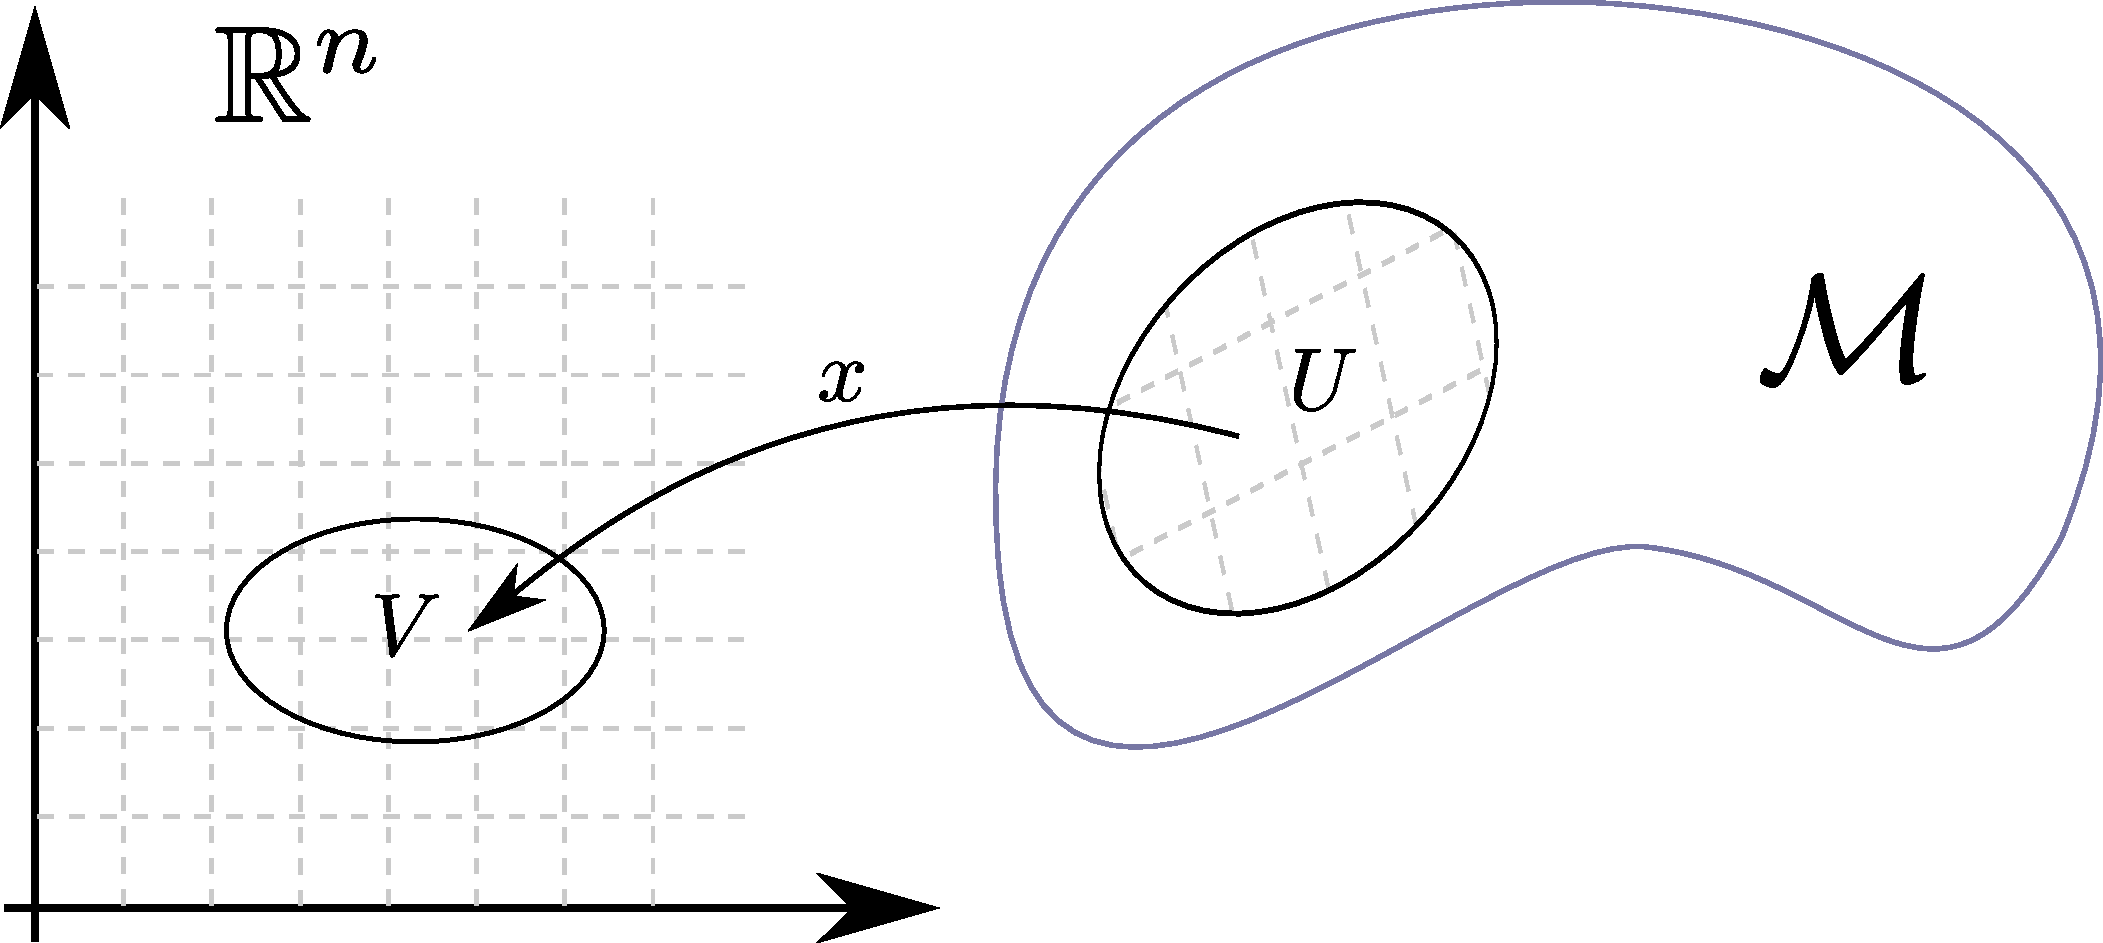
\includegraphics[width=0.7\textwidth]{figurer/coordinate_function.pdf}
    \label{coordinate function}
    \caption{The coordinate function $x$ maps a neighborhood $U$ in the manifold $\Em$ to a negiborhood $V$ in $\R^n$.}
\end{figure}

The most important objects in differential geometry are \emph{smooth manifolds}.
An $n$-dimensional manifold, $\Em$, is a set of points, locally homeomorphic to $\R^n$.
That is, for all points $p \in \Em$, there exists a neighborhood $U$ around $p$, together with a corresponding set of continuous, bijective functions,
%
\begin{align}
    x: U \subseteq \Em & \longmapsto V \subseteq \R^n, \\
    p & \longmapsto x^\mu(p).
\end{align}
%
We call $x(p) = (x^0(p), \dots, x^{n- 1}(p)) = x^\mu(p)$ a coordinate function of $\Em$.
The inverse of $x$, $x^{-1}$, obeys $x^{-1}(x(p)) = p$, for all $p \in U$.
A smooth manifold is one in which the coordinate functions are infinitely differentiable.
To define differentiability on manifolds, consider two coordinate functions, $x$, and $x'$.
The corresponding domains $U$ and $U'$ may or may not overlap.
We then define the transition function, a function between subsets of $\R^n$ by mapping via $\Em$, as
%
\begin{align}
    f_{x\rightarrow x'} = x' \circ x^{-1} : \R^n \mapsto \R^n.
\end{align}
%
The map is illustrated in \autoref{fig: transition map}.
\footnote{To be rigorous, one has to restrict the domains and image of the coordinate function when combining them. This is illustrated in \autoref{fig: transition map}.}
A set of coordinate functions $\mathcal A = \{x_i\}$ whose domain cover $\Em$ is called an \emph{atlas} of $\Em$.
If the transition function between all pairings of coordinate functions in the atlas is smooth---that is, infinitely differentiable---we call the atlas smooth.
We then define a smooth manifold as the topological manifold $\Em$ together with a \emph{maximal} smooth atlas $\mathcal A$.
A smooth atlas is maximal if no coordinate function can be added while the atlas remains smooth.\footnote{%
    The maximal condition ensres that two equivalent atlases correspond to the same differentiable manifold. A single manifold can be combined with different maximal atlases of smooth coordinates or differentiable structures. A set of examples are \emph{exotic spheres}, smooth manifolds which are \emph{homeomorphic} to $\text S^n$, but not \emph{diffeomorphic}. 
    }
%
\begin{figure}[H]
    \centering
    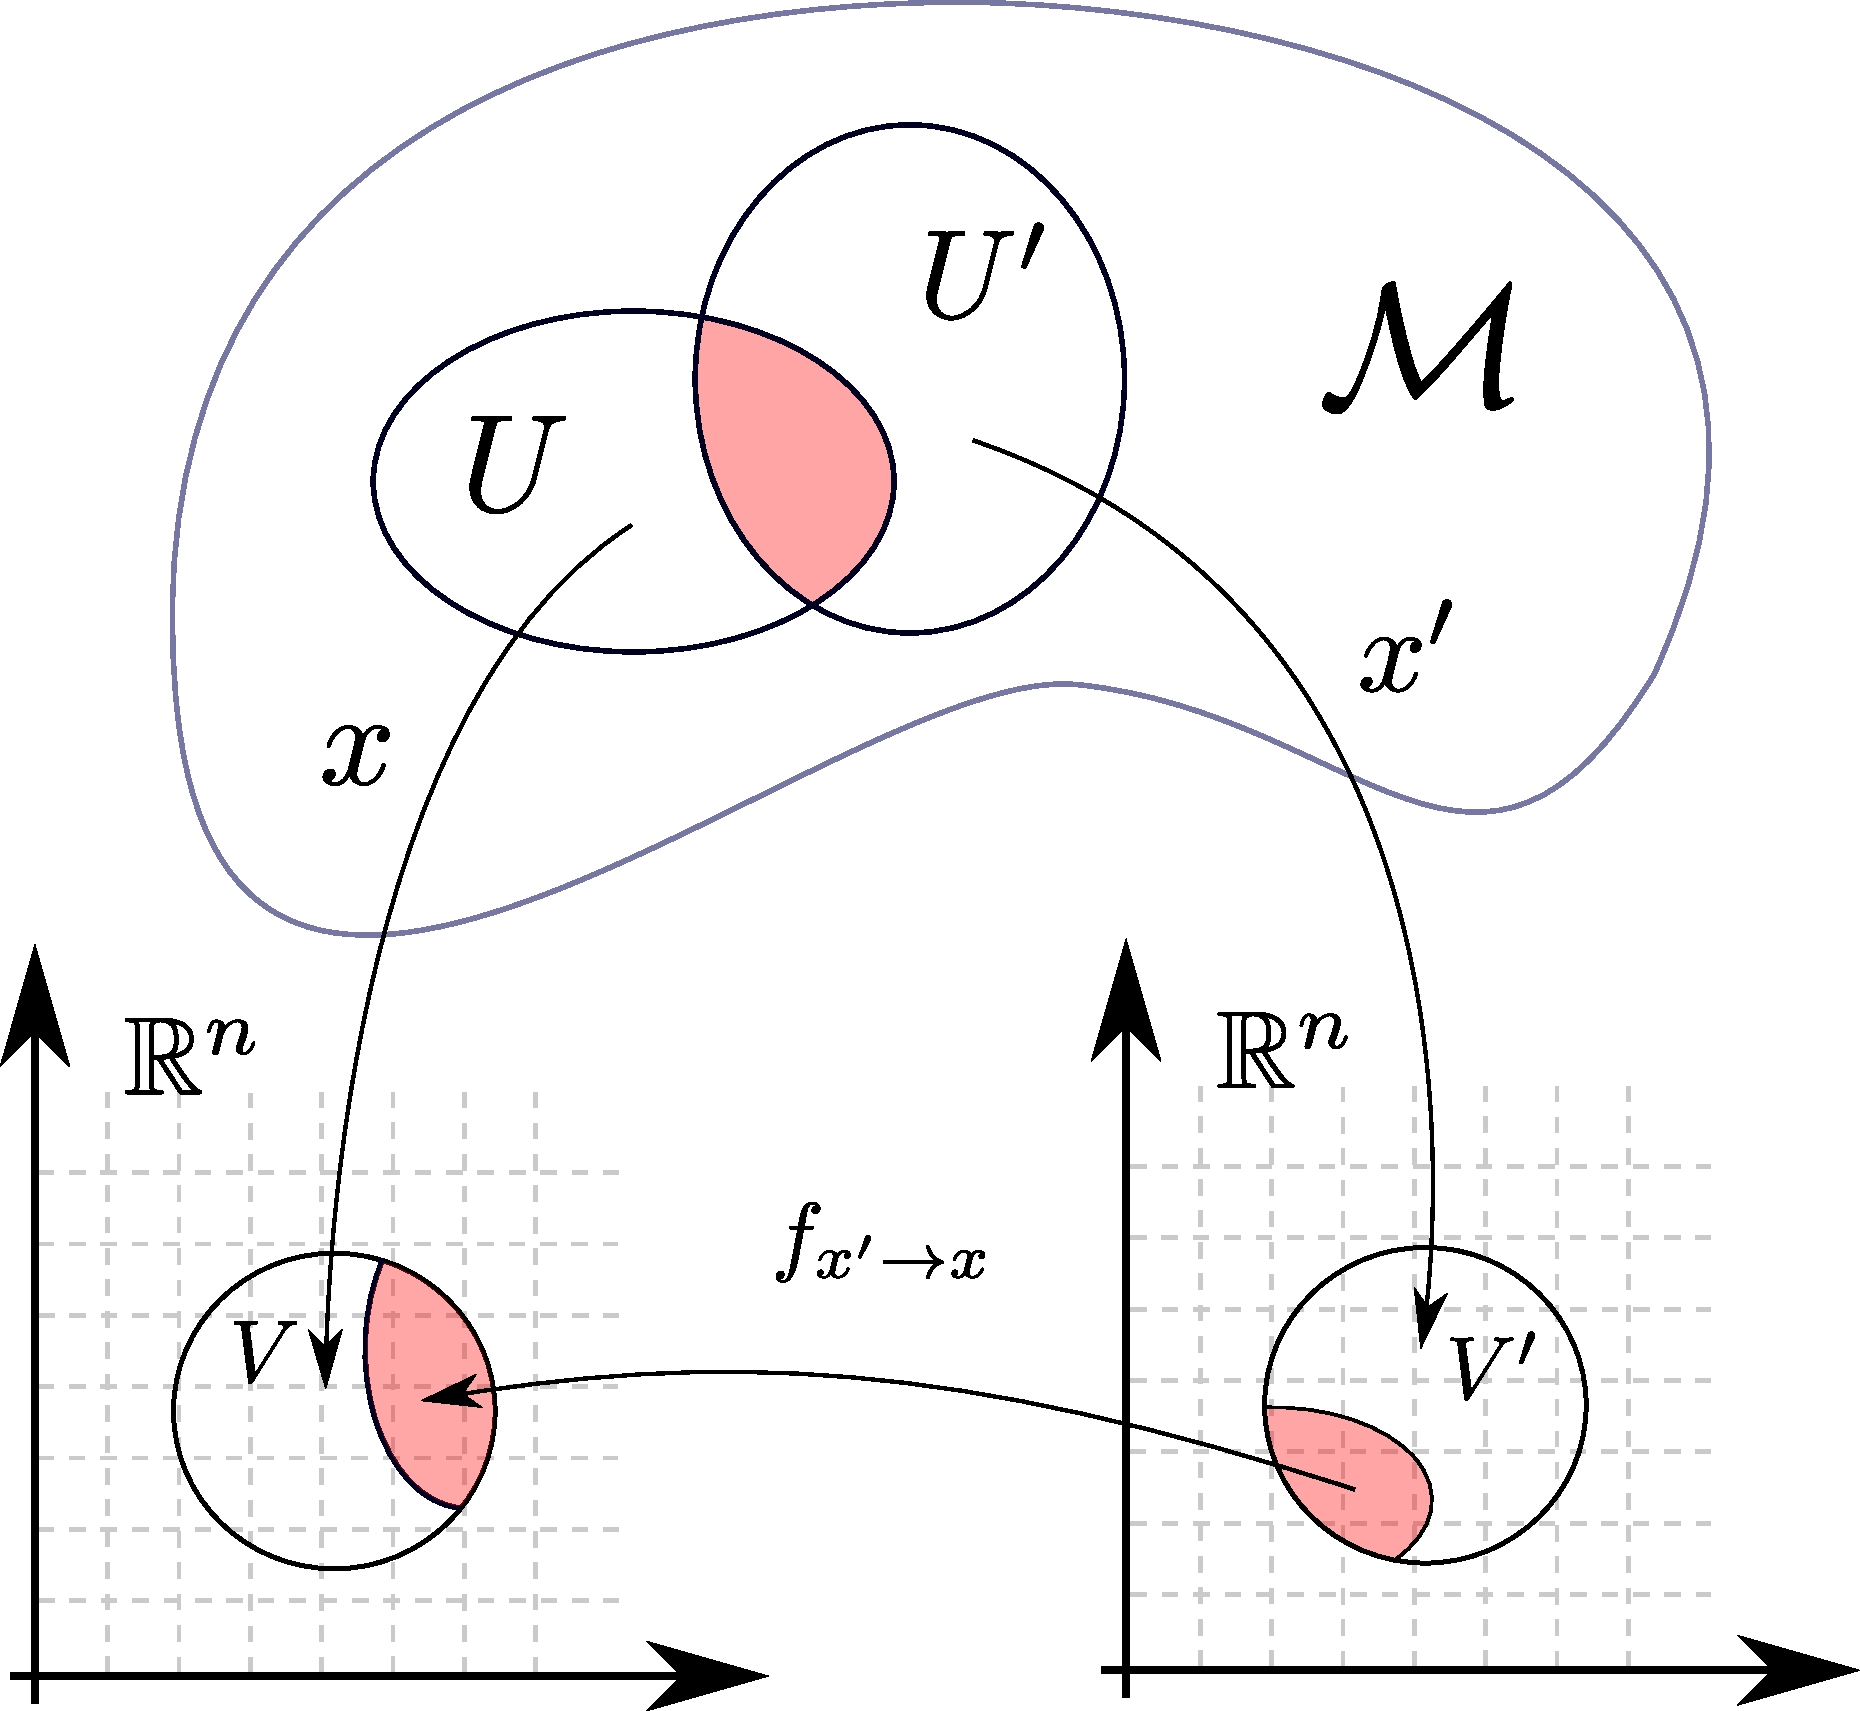
\includegraphics[width=0.6\textwidth]{figurer/transition_map.pdf}
    \caption{
        The transition map $f_{x'\rightarrow x}$ between two coordinate functions, $x$ and $x'$, maps between the images of these function, via the manifold $\Em$. 
        The function's domain and image are restricted to a (possibly empty) subset of the images of $x$ and $x'$. This is illustrated by the shaded regions in $V$ and $V'$. 
        }
    \label{fig: transition map}
\end{figure}

Consider two $m$- and $n$-dimensional smooth manifolds $\Em$ and $\mathcal N$.
Let $x$ denoted the coordinates on $\Em$, while $y$ denotes the coordinates on $\mathcal N$.
We can define smooth functions between these manifolds similarly to how we define smooth coordinates.
Consider the function
%
\begin{equation}
    F: \Em \longmapsto \mathcal N.
\end{equation}
%
It is said to be smooth if, for all points $p \in M$, there is a set of local coordinates $x$ around $p$ and $y$ around $F(p)$ such that the map $\tilde F = y \circ F \circ x^{-1}$ is smooth.
This map may be illustrated by a diagram,
%
\begin{equation}
    % https://tikzcd.yichuanshen.de/#N4Igdg9gJgpgziAXAbVABwnAlgFyxMJZABgBoBGAXVJADcBDAGwFcYkQAdDgW3pwAsARoIAEAJQB63EAF9S6TLnyEUZYtTpNW7LrwEBjJiICys+SAzY8BIuVLqaDFm0SceffocYiAcmYVWyrYUGk7arroewuIShDIaMFAA5vBEoABmAE4Q0oh2IDgQSGQgjPSCMIwACorWKqUw6TggjlouIAAe-iBZOUj5hUgATK3O7OndvbkjBUWIAMyj4SAAnpPZuSWDC0vtSbKUMkA
\begin{tikzcd}
    \mathcal M \arrow[d, "x"] \arrow[r, "F"] & \mathcal N \arrow[d, "y"] \\
    \mathbb R^m \arrow[r, "\tilde F"]               & \mathbb R^n              
    \end{tikzcd}
    %
\end{equation}
%
%
We will not be careful with the distinction between $F$, the function between the abstract manifolds, and $\tilde F$, the function of their coordinates, but rather denote both by $F(x)$.
We may take the partial derivative of such a function with respect to the coordinates $x$, $\pdv{F}/{x^\mu}$.
However, this is dependent on our choice of coordinates, as a set of local coordinates can always be scaled arbitrarily.
Any physical theory must be independent of our choice of coordinates, so our next task is to define the properties of a smooth manifold in a coordinate independent way.


\subsection{Vectors and tensors}

A curve $\gamma$ through $\Em$ is a function from $\R$ to $\Em$,
%
\begin{align}
    \gamma : \R &\longmapsto \Em \\
    \lambda & \longmapsto \gamma(\lambda).
\end{align}
%
Such curves are often denoted only by their coordinates and the parameter $\lambda$, $x^\mu(\lambda) = (x^\mu \circ \gamma)(\lambda)$.
With this curve, we can take the directional derivative of a real-valued function on the manifold, $f: \Em \mapsto \R$.
Assume $\gamma(\lambda = 0) = p$.
As we are always taking the derivative of functions between $\R^n$, for different $n$, we can use the chain rule.
The directional derivative of $f$ at $p$, given by this curve $\gamma$, is then
%
\begin{equation}
    \odv{}{\lambda} f(x(\lambda)) \bigg |_p = \odv{x^\mu}{\lambda} \bigg |_{\lambda = 0}  \pdv{}{x^\mu} f(x) \bigg |_p.
\end{equation}
%
The set of all such directional derivatives, $\odv{}/{\lambda}$ at $p$, form a vector space, $T_p \Em$, called the \emph{tangent space}.
The tangent space is illustrated in \autoref{fig: tangent space}.
The coordinates $x^\mu$ induce a basis of this vector space, namely partial derivatives with respect to the coordinate functions at $p$
%
\begin{equation}
    e_\mu = \pdv{}{x^\mu} \bigg|_p = \partial_\mu|_p, \quad \mu \in \{0, ... n-1\}.
\end{equation}
%
Any element $v \in T_p \Em$ can therefore be written
%
\begin{equation}
    v = v^\mu \partial_\mu |_p = \odv{x^\mu}{\lambda}\Big |_{\lambda = 0} \pdv{}{x^\mu}\Big |_p.
\end{equation}
%
Here, $\lambda$ is the parameter of the curve corresponding to the directional derivative $v$.\footnote{%
There is not only one curve corresponding to any directional derivative but rather an equivalence class. We will gloss over this technicality, as it does not affect our work.
}
The evaluation at $\lambda = 0$ and $p$ will often be implicit for ease of notation.
This directional derivative acts on functions $f : \Em \mapsto \R$ as
%
\begin{equation}
    v(f) = v^\mu \partial_\mu f.
\end{equation}
%

\begin{figure}[ht]
    \centering
    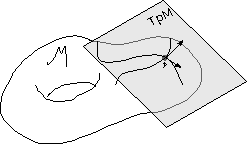
\includegraphics[width=0.7\textwidth]{figurer/tangent space.pdf} 
    \caption{
        (Kladd) The tangent space $T_p \Em$, the shaded rectangle, is the sett of all directional derivatives at $p\in \Em$. A directional derivative is defined in terms of a curve that passes through $p$.
        } 
    \label{fig: tangent space}
\end{figure}



A map $F$ between two manifolds $\Em$ and $\mathcal N$ also induces a map between the tangent spaces of these manifolds.
This is the \emph{differential} of $F$ at $p$, 
%
\begin{align}
    \dd F_p: T_p \Em & \longmapsto T_p \mathcal N, \\
    v & \longmapsto \dd F_p (v). 
\end{align}
%
As $\dd F_p(v)$ is an element of $T_p \mathcal N$,   directional derivative on $\mathcal N$, defined as
%
\begin{equation}
    \dd F_p(v) (g) = v(g \circ F),
\end{equation}
%
for functions $g : \mathcal N \mapsto \R$.
It thus acts on functions on $\mathcal N$ by ``extending'' the derivative $v$.
This is a linear map between vector spaces and may be written in component form by considering the differentials of the coordinate functions.
Denote the coordinates of $\mathcal N$ by $y^\mu$, and $y^\mu \circ F = F^\mu$.
Then,
%
\begin{equation}
    \dd F_p (\partial_\mu) (g) = \partial_\mu (g \circ F) |_p 
    = \pdv{F^\nu}{x^\mu}\Big |_p \pdv{g}{y^\nu} \Big  |_{F(p)},
\end{equation}
%
or more suggestively
%
\begin{equation}
    \dd F \left( \pdv{}{x^\mu} \right) = \pdv{F^\nu}{x^\mu} \pdv{}{y_\nu}.
\end{equation}
%
This is a linear map of vectors between two vectors by the matrix $A_\mu{}^\nu = \partial_\mu F^\nu$.
The differential is thus a generalization of the Jacobian.
In the case of a real valued function, $f: \Em \mapsto \R$, and $g : \R \mapsto \R$, we get
%
\begin{equation}
    \dd f (v) (g) 
    = v(g \circ f) 
    = (v^\mu \partial_\mu f) \, \odv{g}{y}.
\end{equation}
%
$\dd f$ is thus a map from $T_p \Em$ to $T_{f(p)}\R$, which is isomorphic to $\R$.
The $g$ be the identity function, so that $\odv{g}/{y} = 1$.
Then, the differential of a scalar function, also called a 1-form, is a map from vectors $v$ to real numbers,
%
\begin{equation}
    \label{covectors i.e. one forms}
    \dd f(v) := v^\mu \partial_\mu f.
\end{equation}
%
The set of all linear maps from a vector space $V$ to the real numbers is called the \emph{dual space} of $V$, denoted $V^*$.
This is a new vector space with the same dimensionality as $V$.
We denote the dual of $T_p \Em$ as $T_p^* \Em$.
We can regard each coordinate function as a real-valued function with a corresponding differential.
This differential obeys
%
\begin{equation}
    \dd x^\mu (\partial_\nu) = \pdv{x^\mu}{x_\nu} = \delta^\mu_\nu.
\end{equation}
%
The differentials of the coordinate functions thus form a basis for $T^*_p \Em$, called the dual basis.
Any differential $\dd f$ can thus be written as $\dd f = \omega_\mu \dd x^\nu$ for some components $\omega_\mu$.
We finde the components by applying the differential to the coordinate basis, $\dd f(\partial_\mu) = \partial_\mu f = \omega_\mu$.
In other words, we recover the classical expression 
%
\begin{equation}
    \dd f = \pdv{f}{x^\mu} \dd x^\mu,
\end{equation}
however we now interpret it as a covector-field instead of an ``infinitesimal displacement''.

Linear maps from vectors to real numbers is generalized by \emph{tensors}.
Given a vector space $V$, a general $(n, m)$ tensor $T$ is a multilinear map, which associates $n$ elements from $V$ and $m$ from its dual $V^*$ to the real numbers, i.e.,
%
\begin{align}
    T: V \times V \times \dots\times V^* \times \dots &\longmapsto \R, \\
    (v, u\dots; \omega, \dots) & \longmapsto T(v, u, \dots; \omega, \dots).
\end{align}
%
Multilinear means that $T$ is linear in each argument.
The set of all such maps is the tensor product space $V\otimes V \otimes \dots \otimes V^* \otimes \dots$, a $\dim(V)^{n+m}$-dimensional vector space.
If $\{e_\mu\}$ and $\{e^\mu\}$ are the basis for $V$ and $V^*$, then we can write the basis of this of the tensor product space as $ \{e_{\mu} \otimes\dots \otimes e^{\nu} \otimes \dots \}$.
The tensor can thus be written
%
\begin{equation}
    T =
     T^{\mu \nu\dots}{}_{\rho\dots} \, e_{\mu}\otimes e_\nu \otimes \dots e^\rho\otimes\dots, \quad
    T^{\mu \nu\dots}{}_{\rho\dots} = T(e^\mu, e^\nu, \dots; e_\rho, \dots).
\end{equation}
% 
We often what to decopose a tensor down into its symmetric and antisymmetric parts.
To do this, we introduce the symmetrization of a tensor $T$, 
%
\begin{equation}
    T_{(\mu_1\dots\mu_n)} 
    = \frac{1}{n!} \sum_{\sigma \in S_n} 
    T_{\mu_{\sigma(1)} \dots \mu_{\sigma(n)}},
\end{equation}
%
where $S_n$ is the set of all permutations of $n$ objects.
The antisymmetrization of a tensor is defined as
%
\begin{equation}
    T_{[\mu_1\dots\mu_n]} 
    = \frac{1}{n!} \sum_{\sigma \in S_n} \text{sgn}(\sigma)  
    T_{\mu_{\sigma(1)} \dots\mu_{\sigma(n)}}.
\end{equation}
%
The function $\text{\sigma} = \pm 1$, depending on if $\sigma$ is a even or odd permutation.
We may now write
%
\begin{equation}
    T_{\mu \nu} = T_{(\mu \nu)} + T_{[\mu \nu]}.
\end{equation}


\subsection{Geometry and the metric}
\label{subsection: goemetry and the metric}

The metric is a symmetric, non-degenerate $(0, 2)$ tensor
%
\begin{equation}
    \dd s^2 = g_{\mu \nu} \, \dd x^\mu \otimes \dd x^\nu.
\end{equation}
%
It defines the geometry of the manifold $\Em$, and is the main object of study in general relativity.
As it is invertible, we can define $g^{\mu \nu} = (g^{-1})_{\mu \nu}$, which is the components of a $(2, 0)$ tensor.
We use this to raise and lower indices, as is done with the Minkowski metric $\eta_{\mu \nu}$ in special relativity.

Up until now, we have only considered the tangent space $T_p \Em$ at a point $p$ and the corresponding tensor-product spaces.
We are, however, more interested in \emph{fields} of vectors, covectors, or tensors.
For each point $p \in \Em$, a tensor field $T$ ``picks out'' a tensor $T(p)$ from each tensor product space corresponding to the tangent space at $p$, $T_p \Em$.
We will use a vector field to illustrate.
This vector field can be written as
%
\begin{equation}
    v(p) = v^\mu(p) \partial_\mu |_p. 
\end{equation}
%
We will mostly be working with the components $v^\mu$, which are functions of $\Em$.
For ease of notation, we write the vector as a function of the coordinates $x$.
The vector field $v(x)$ is unchanged by a coordinate-transformation $x^\mu \rightarrow {x'}^\mu$; the coordinates are only a tool for our convenience.
However, with a new set of coordinates, we get a new set of basis vectors, $\partial'_\mu$:
%
\begin{equation}
    v = v^\mu \partial_\mu = v^\mu \pdv{x'^\nu}{x^\mu} \partial'_\nu
    = v'^\mu \partial_\mu',
\end{equation}
%
This gives us the transformation rules for the components of vectors,
%
\begin{equation}
    v'^\mu = \pdv{x'^\mu}{x^\nu} v^\nu.
\end{equation}
%
Tangent vectors are also called \emph{contravariant} vectors, as their components transform contra to basis vectors.
For covectors, it is
%
\begin{equation}
    \omega'_\mu = \pdv{x^\nu}{x'^\mu} \omega_\nu,
\end{equation}
%
which is why covectors also are called \emph{covariant} vectors.

The gradient of a scalar function $f$, $\dd f = \partial_\mu f \dd x^\mu$, is a coordinate-independent derivative, as $\partial_\mu f$ follows the transformation law for covectors.
We define the covariant derivative, $\nabla$, as a map from $(n, m)$ tensor fields to $(n, m+1)$ tensor fields.
When considering a scalar as a $(0, 0)$ tensor, we see that this generalizes the scalar derivative.
The components of a covariant derivative, $\nabla_\rho T^{\mu_1\dots}{}_{\nu_1, \dots}$, must follow the tensor transformation law. 
However, this is not strong enough to uniquely define $\nabla$.
We further assume
%
\begin{itemize}
    \item Linearity: $\nabla (T + S) = \nabla T + \nabla S$.
    \item The product rule: $\nabla (T \otimes S) = (\nabla T)\otimes S + T \otimes (\nabla S)$.
    \item Reduces to partial derivative for scalars: $\nabla_\mu f = \partial_\mu f$.
    \item Kronecker delta gives zero: $\nabla_\mu \delta^\rho_\nu = 0$.
\end{itemize}
%
With this, we can, in general, write the covariant derivative as~\autocite{carrollSpacetimeGeometryIntroduction2019}
%
\begin{align}
    \label{covariant derivative diff geom}
    \nabla_\mu v^\nu &= \partial_\mu v^\nu + \Gamma^\mu_{\nu \rho} v^\rho, \\
    \label{covariant derivative diff geom covector}
    \nabla_\mu \omega_\nu &= \partial_\mu \omega_\nu - \Gamma^\rho_{\mu \nu} \omega_\rho,
\end{align}
%
for vectors and covectors.
$\Gamma^{\mu}_{\nu \rho}$ are called \emph{Christoffel symbols}.
The generalization for higher-order tensors is straightforward, 
%
\begin{equation}
    \nabla_\mu T^{\nu\dots}{}_{\rho\dots}
    =
    \partial_\mu T^{\nu\dots}{}_{\rho\dots}
    + \Gamma^\mu_{\nu \lambda} T^{\lambda\dots}{}_{\rho\dots} +\dots
    - \Gamma^\lambda_{\mu \rho} T^{\mu\dots}{}_{\lambda\dots} -\dots.
\end{equation} 
%
This is still not enough to uniquely determine the covariant derivative.
We will furthermore assume $\Gamma^{\lambda}_{\mu \nu} = \Gamma^{\lambda}_{\nu \mu}$ and $\nabla_\mu g_{\nu \rho} = 0$.
With these, we can find an explicit formula of the Christoffel symbols in terms of the metric,
%
\begin{equation}
    \label{christoffel symbols from metric}
    \Gamma^\rho_{\mu \nu} = \frac{1}{2} g^{\rho \sigma} (\partial_\mu g_{\nu \sigma} - \partial_\sigma g_{\mu \nu} + \partial_{\nu}g_{\sigma \mu}).
\end{equation}
%
With the notion of a covariant derivative, we may also generalize \emph{parallel transport} to curved spaces.
The notion of parallel transport of a vector in flat $\R^n$ is intuitive---given a line $x^\mu(\lambda)$, a vector $v^\mu$ at $x^\mu(\lambda_0)$ is parallel transported to $v'^\mu$ at $x^\mu(\lambda_1)$ if they ``point in the same direction''.
To make this more precise, a vector field $v^\mu$ is parallel transported along $x^\mu(\lambda)$ if $\odv{}{\lambda} v^\mu = \odv{x^\nu}{\lambda} \partial_\nu v^\mu$ = 0.
We generalize this to curved spaces by replacing the partial derivative with a covariant derivative, and so the criterion for parallel transport is
%
\begin{equation}
    \label{parallel transport criterion}
    \odv{x^\mu}{\lambda} \nabla_\mu v^\nu = 0.
\end{equation}
%
With this, we can imagine creating a special class of paths, called \emph{geodesics}, namely those which parallel transport their tangent vectors $\odv{x^\mu}{\lambda}$.
We imagine following an arrow we are holding without turning it as we walk.
Using the definition of parallel transport \autoref{parallel transport criterion}, together with the covariant derivative \autoref{covariant derivative diff geom}, we get the geodesic equation,
%
\begin{equation}
    \label{goedesic equation}
    \odv[2]{x^\mu}{\lambda} 
    + \Gamma^\mu_{\rho \sigma} \odv{x^\rho}{\lambda} \odv{x^\rho}{\lambda}
    = 0.
\end{equation}
In a flat space, where the Christoffel symbols vanish, this reduces to the familiar criterion for straight lines, $\odv[2]{x^\mu}{\lambda} = 0$.

The curvature of a manifold $\Em$, with the metric $g_{\mu \nu}$, is encoded in the Riemann tensor.
It is defined by
%
\begin{equation}
    \label{Riemann tensor}
    [\nabla_\mu, \nabla_\nu] v^\rho = R^{\rho}{}_{\sigma \mu \nu} v^\sigma,
\end{equation}
%
which in our case gives the explicit formula
%
\begin{equation}
    \label{riemann tensor in terms of christoffel symbols}
    R^\rho{}_{\sigma \mu \nu} 
    = \partial_{\mu} \Gamma^{\rho}_{\nu \sigma}
    - \partial_{\nu} \Gamma^{\rho}_{\mu \sigma}
    + \Gamma^{\rho}_{\mu \lambda} \Gamma^{\lambda}_{\nu \sigma}  
    - \Gamma^{\rho}_{\nu \lambda} \Gamma^{\lambda}_{\mu \sigma}.
\end{equation}
%
Although the Christoffel symbols are not tensors, the Riemann tensor is due to its definition using covariant derivatives.
We can therefore contract some of its indices to get other tensor quantities.
We  efine the Ricci tensor and Ricci scalar as
%
\begin{align}
    \label{Ricci tensor}
    R_{\mu \nu} &= R^{\rho}{}_{\mu \rho \nu}, \\
    \label{Ricci scalar}
    R &= R^{\mu}{}_{\mu} = g^{\mu \nu} R_{\mu \nu}.
\end{align}
%
This form gives us several useful identities, such as
%
\begin{equation}
    R_{\rho \sigma \mu \nu} 
    = 
    R_{[\rho \sigma] \mu \nu}
    =
    R_{\rho \sigma [\mu \nu]}
    =
    R_{\mu \nu \rho \sigma }.
\end{equation}
%
Using the Jacobi identity of the commutator, we have
%
\begin{equation}
    \label{Jacobi identity differential geometry}
    [\nabla_\mu, [\nabla_\nu, \nabla_\sigma]]
    + [\nabla_\sigma, [\nabla_\mu, \nabla_\nu]]
    + [\nabla_\nu, [\nabla_\sigma, \nabla_\mu]] = 0.
\end{equation}
%
If we apply this on $\delta^{\mu}_{\nu}$, we get the differential Bianchi identity, compactly written
%
\begin{equation}
    \label{Binachi identiy}
    \nabla_{[\mu}R_{\nu \rho]\sigma \eta} = 0.
\end{equation}
%
To interpret the Riemann tensor, we define the parallel propagator $P$.
A vector that is parallel transported along a curve parametrized by $\lambda$, so that $v^\mu(\lambda)$ obey the criterion of parallel transport \autoref{parallel transport criterion}, obey
%
\begin{equation}
    v^\mu(\lambda) = P^\mu{}_\nu(\lambda) v^\nu.
\end{equation}
%
Inserting this into the equation for parallel transport, \autoref{parallel transport criterion}, this operator must obey
%
\begin{equation}
    \odv{}{\lambda} P^\mu{}_\nu = - \Gamma^\mu_{\rho \sigma}  \odv{x^\rho}{\lambda}P^\sigma{}_\nu.
\end{equation}
%
This has the same form as the definition of the unitary time-evolution operator in quantum mechanics, and we could therefore write down a solution involving an exponential and a path ordering operator, $\mathcal P$, analogous to the time ordering operator from quantum mechanics.
We may rewrite the equation as an integral equation,
%
\begin{equation}
    P^\mu{}_\nu(\lambda) = \delta^\mu_\nu 
    - \int^\lambda_0 \dd \lambda' \Gamma^\mu_{\rho \sigma} V^\rho P^\sigma{}_\nu,
\end{equation}
%
where we denote $\odv{x^\mu}{\lambda} = V^\mu$.
This allows us to solve the equation iteratively.
If $\lambda \leq \epsilon \ll 1$, then we would expect this to converge, as long as the $g$ is well-behaved.
In that case, we can start with the zeroth-order solution $P^{\mu}{}_\nu = \delta^\mu_\nu$, then iterate twice to obtain
%
\begin{equation}
    \label{iterative paralell propagator}
    P^\mu{}_\nu(\lambda) 
    = 
    \delta^\mu_\nu 
    - \int_0^\lambda \dd \lambda' \, 
    \Gamma^\mu_{\rho \nu} V^\rho
    + \int_0^{\lambda} \dd \lambda ' \int_0^{\lambda'} \dd \lambda ''\,
    \Gamma^\mu_{\rho \sigma} \Gamma^\sigma_{\eta \nu} V^\rho V^\eta
    + \Oh(\epsilon^3).
\end{equation}
%
With this, we will investigate how much a vector $v^\mu$ is changed by being parallel transported around in a small loop.
This is illustrated in \autoref{fig: parallel transport in loop}.
%
\begin{figure}
    \centering
    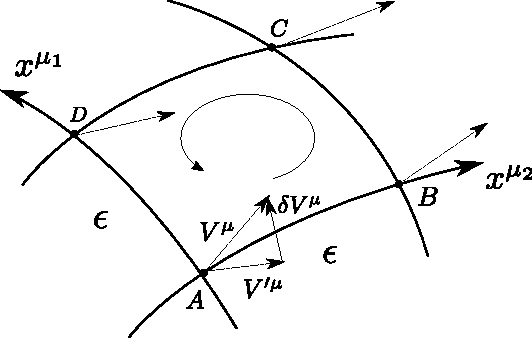
\includegraphics[width=0.7\textwidth]{figurer/parallel_transport.pdf}
    \caption{A vector $v^\mu$ is parallel transported in a small, closed loop, defined by the coordinate functions $x^{\mu_1}$ and $x^{\mu_2}$.
    As a consequence of the curvature, it has changed by $\delta v^\mu$ by the time it arrives back at $A$.}
    \label{fig: parallel transport in loop}
\end{figure}
%
A vector $v^\mu$, is parallel transported in a loop along the coordinate lines.
These lines are where either of the coordinate functions $x^{\mu_1}$ or $x^{\mu_2}$ are equal to $0$ or $\epsilon$.
Here, the indices $\mu_1$ and $\mu_2$ are not free, but identify the two coordinate functions which define this loop.
The line from $A$ to $B$, defined by $x^{\mu_1} = 0$, is parametrized by $x^\mu(\lambda) = \lambda \delta^\mu_{\mu_2}$, so $ V^\mu = \delta^\mu_{\mu_2} $.
The Christoffel symbol along this line is
%
\begin{equation}
    \Gamma^{\mu}_{\nu \rho}(\lambda) 
    = \Gamma^{\mu}_{\nu \rho}|_A
    + \lambda \partial_{\mu_2} \Gamma^{\mu}_{\nu \rho}|_A + \Oh(\lambda^2).
\end{equation}
%
Inserting this into \autoref{iterative paralell propagator}, we get
%
\begin{equation}
    P^\mu{}_\nu(\epsilon)
    = \delta^\mu_\nu 
    - \epsilon \Gamma^{\mu}_{\nu \mu_2}|_A
    + \frac{1}{2} \epsilon^2 
    \left(
        \Gamma^\mu_{\mu_2 \sigma}\Gamma^\sigma_{\mu_2 \nu} |_A 
        -\partial_{\mu_2} \Gamma^{\mu}_{\nu \mu_2}|_A 
    \right)
    + \Oh(\epsilon^3).
\end{equation}
%
Next, from $B$ to $C$, the line is $x^\mu(\lambda) = \epsilon \delta^\mu_{\mu_2} + \lambda \delta^{\mu}_{\mu_1}$, so $V^\mu = \delta^\mu_{\mu_1}$, and the Christoffel symbols are 
$ 
\Gamma^{\mu}_{\nu\rho}
= 
\Gamma^{\mu}_{\nu \rho}|_B
+ \lambda \partial_{\mu_1} \Gamma^{\mu}_{\nu \rho}|_B
$
to fist order in $\lambda$.
Here, we have to expand once more to evaluate the symbols at $A$.
Then, we get
%
\begin{equation}
    \Gamma^{\mu}_{\nu\rho}
    =
    \Gamma^{\mu}_{\nu \rho}|_A + \epsilon \partial_{\mu_2} \Gamma^{\mu}_{\nu \rho}|_A
    + \lambda \partial_{\mu_1} \Gamma^{\mu}_{\nu \rho}|_A,
\end{equation}
%
The parallel propagator from $B$ to $C$ is then
%
\begin{equation}
    P^{\mu}{}_\nu(\epsilon)
    = 
    \delta^\mu_\nu
    - \epsilon \Gamma^{\mu}_{\nu \mu_1}|_A 
    + \frac{1}{2}\epsilon^2
    \left(
        \Gamma^\mu_{\sigma \mu_1}\Gamma^\sigma_{\nu \mu_1}|_A
        - \partial_{\mu_1} \Gamma^{\mu}_{\nu \mu_1}|_A
        - 2 \partial_{\mu_2} \Gamma^{\mu}_{\nu \mu_1}|_A
    \right).
\end{equation}
%
The combined propagator from $A$ to $C$ is then, to second order in $\epsilon$, 
%
\begin{align}
    \nonumber
    {P_{AC}}^\mu{}_{\nu}
    & = 
    \left[ 
        \delta^\mu_\sigma 
        -\epsilon \Gamma^{\mu}_{\sigma \mu_1}
        + \frac{1}{2} \epsilon^2 
        \left(
        \Gamma^\mu_{\eta \mu_1}\Gamma^\eta_{\sigma \mu_1}
        - \partial_{\mu_2} \Gamma^{\mu}_{\sigma \mu_2}
        - 2 \partial_{\mu_2} \Gamma^{\mu}_{\sigma \mu_1}
        \right)
    \right]
    \cdot 
    \left[
        \delta^\sigma_\nu
        - \epsilon \Gamma^{\sigma}_{\nu \mu_2}
        + \frac{1}{2} \epsilon^2 
        \left(
            \Gamma^\sigma_{\eta \mu_2}\Gamma^\eta_{\nu \mu_2}
            - \partial_{\mu_2} \Gamma^{\sigma}_{\nu \mu_2}
        \right)
    \right] \\ \nonumber
    & =
    \delta^\mu_\nu
    - \epsilon 
    \left(
        \Gamma^{\mu}_{\nu \mu_1}
        +
        \Gamma^{\mu}_{\nu \mu_2}
    \right)
    + \epsilon^2
    \frac{1}{2}
    \left(  
        2\Gamma^{\mu}_{\sigma \mu_1} \Gamma^{\sigma}_{\nu \mu_2}
        + \Gamma^\mu_{\sigma \mu_1}\Gamma^\sigma_{\nu \mu_1}
        + \Gamma^\mu_{\sigma \mu_2}\Gamma^\sigma_{\nu \mu_2}
        - 2 \partial_{\mu_2} \Gamma^{\mu}_{\nu \mu_1}
        - \partial_{\mu_1} \Gamma^{\mu}_{\nu \mu_1}
        - \partial_{\mu_2} \Gamma^{\mu}_{\nu \mu_2}
    \right).
\end{align}
%
The parallel propagator for $CDA$ is the propagator for $ADC$ with its signs flipped. 
The $ADC$ propagator is the same as $ABC$, only with the $\mu_1$ and $\mu_2$ indices switched.
It is thus
%
\begin{align}
    \nonumber
    {P_{CA}}^\mu{}_\nu
    & =
    \delta^\mu_\nu
    + \epsilon 
    \left(
        \Gamma^{\mu}_{\nu \mu_2}
        +
        \Gamma^{\mu}_{\nu \mu_1}
    \right)
    + \epsilon^2
    \frac{1}{2}
    \left(  
        2\Gamma^{\mu}_{\sigma \mu_2} \Gamma^{\sigma}_{\nu \mu_1}
        + \Gamma^\mu_{\sigma \mu_2}\Gamma^\sigma_{\nu \mu_2}
        + \Gamma^\mu_{\sigma \mu_1}\Gamma^\sigma_{\nu \mu_1}
        + 2 \partial_{\mu_1} \Gamma^{\mu}_{\nu \mu_2}
        + \partial_{\mu_2} \Gamma^{\mu}_{\nu \mu_2}
        + \partial_{\mu_1} \Gamma^{\mu}_{\nu \mu_1}
    \right).
\end{align}
%
The full propagator, from $A$ to $A$, is $P^\mu{}_\nu = {P_{CA}}^\mu{}_\rho {P_{AC}}^\rho{}_\nu$.
The terms linear in $\epsilon$ vanish, and the same with the terms with two equal $\mu_i$-indices.
The change in the vector as it is rotated around the loop is therefore, to second order in $\epsilon$,
%
\begin{align}
    \delta v^\mu 
    = P^\mu{}_\nu v^\nu - v^\mu 
    = \epsilon^2  
    \left(
        \Gamma^\mu_{\sigma \mu_1} \Gamma^\sigma_{\nu \mu_2}
        -\Gamma^\mu_{\sigma \mu_2} \Gamma^\sigma_{\nu \mu_1}
        + \partial_{\mu_1} \Gamma^{\mu}_{\nu \mu_2}
        - \partial_{\mu_2} \Gamma^{\mu}_{\nu \mu_1} 
    \right) v^\nu.
\end{align}
Comparing with \autoref{riemann tensor in terms of christoffel symbols}, we see that this is the Riemann curvature tensor.
In other words, the Riemann tensor encodes how a vector is transformed when parallel transported in a small, closed loop.



\subsection{Integration on manifolds}
\label{subsection: integration on manifolds}

The integral of a scalar function on a manifold is not a coordinate-independent notion, and we must introduce the notion of $n$-forms.
A $n$-form is a antisymmetric $(0, n)$ tensor.
The wedge product, $\wedge$ is a product which maps two $n$- and $m$-forms to a $n+m$-form, and is defined as
%
\begin{equation}
    (A\wedge B)_{\mu_1\dots\mu_{n+m}} = \frac{(n + m)!}{n! m!} A_{[\mu_1\dots\mu_n}B_{\mu_{n+1}\dots\mu_{n+m}]},
\end{equation}
%
A $n$-form $\omega$ may now be written as
%
\begin{equation}
    \omega 
    = \omega_{[\mu_1 \dots \mu_n]} \, \dd x^{\mu_1} \otimes \dots \otimes \dd x^{\mu_n}
    = \omega_{\mu_1 \dots \mu_n} \, \dd x^{\mu_1} \wedge \dots \wedge \dd x^{\mu_n}.
\end{equation}
% 
Furthermore, we define the exterior derivative, a map from $n$-forms to $n+1$-forms, defined by
%
\begin{equation}
    (\dd T)_{\mu_1 \dots \mu_{n+1}} = (n+1) \partial_{[\mu_1} T_{\mu_2\dots\mu_{n+1}]}.
\end{equation}
%
We are interested in a coordinated independent quantity that we can integrate over.
To that end, we define
%
\begin{equation}
    \dd^n x := \dd x^0 \wedge \dots \wedge \dd x^{n-1}
    = \frac{1}{n!} \varepsilon_{\mu_1 \dots \mu_n}  
    \dd x^{\mu_1} \wedge \dots \wedge \dd x^{\mu_n},
\end{equation}
%
Where $\varepsilon_{\mu_1 \dots \mu_n}$ is the Levi-Civita symbol.
Given a different set of coordinates, $x'^\mu$, these are related by
%
\begin{equation}
    \dd^n x = \det\left( \pdv{x}{x'} \right) \, \dd^n x',
\end{equation}
%
where we have used the relation $\varepsilon_{\mu_1 \dots \mu_n}  \det(A) = \varepsilon_{\nu_1 \dots \nu_n} A^{\nu_1}{}_{\mu_1} \dots A^{\nu_n}{}_{\mu_n}$.  
We define $|g| = |\det(g_{\mu \nu })|$, which, by the transformation properties of tensors, transforms as
%
\begin{equation}
    \sqrt{|g'|} = \left| \det\left(\pdv{x'}{x} \right) \right| \sqrt{|g'|},
\end{equation}
%
This means that we can use this to compensate for the transformation of $\dd^n x$, and get a volume form with a coordinate independent expression,
%
\begin{equation}
    \dd V = \sqrt{|g|} \, \dd^n x = \sqrt{|g'|} \, \dd^n x'.
\end{equation}
%
With this, we can integrate scalars in a well-defined way by mapping them to a corresponding $n$-form, $f \rightarrow f \dd V$.
We define the integral of a scalar function $f$ on a manifold $\Em$ with a metric $g$ as
%
\begin{equation}
    I = \int_\Em \dd V \, f =  \int_{\Em} \dd^n x \, \sqrt{|g(x)|} \, f(x).  
\end{equation}


Stoke's theorem generalizes the fundamental theorem of calculus and the divergence theorem to manifolds.
Let $\Em$ be a differential manifold of dimension $n$, with the boundary $\partial \Em$.
Stoke's theorem says that, for an $n-1$-form $\omega$,
%
\begin{equation}
    \int_\Em \dd \omega = \int_{\partial \Em}  \omega. 
\end{equation}

Stoke's theorem then implies a generalized divergence theorem.
The boundary of $\Em$ is a $n-1$ manifold dimensional, and a metric $g$ on $\Em$ will induce a new metric $\gamma$ on $\partial \Em$.
This metric corresponds to the restriction of $g$ to $\partial \Em$.
Furthermore, there will be a vector field $n^\mu$ of normalized vectors orthogonal to all elements of $T \partial \Em$.
This theorem states that for a vector field $V^\mu$ on $\Em$,
%
\begin{equation}
    \label{generalized divergence theorem}
    \int_\Em \dd^n x \, \sqrt{|g|} \,  \nabla_\mu V^\mu 
    = \int_{\partial \Em} \dd^{n-1}y \, \sqrt{|\gamma|} \, n_\mu V^\mu.
\end{equation}

    \section{*Lie groups}

This section is based on~\autocite{leeIntroductionSmoothManifolds2003d,peskinIntroductionQuantumField1995,schwartzQuantumFieldTheory2013,weinbergQuantumTheoryFields1995,weinbergQuantumTheoryFields1996}.


\subsection{Groups}
Lie groups are a natural structure to capture the symmetries of a physical theory.
A Lie group is a smooth manifold, with the additional structure of a \emph{group}.
A group is a set, $G$, together with a map
%
\begin{align}
    (\cdot, \cdot):  G \times G &\longmapsto G ,\\
    (g_1, g_2) &\longmapsto g_3,
\end{align}
% 
called group multiplication. This map obeys the group axioms, which are the existence of an identity element $\one$, associativity and the existence of an inverse element $g^{-1}$ for all $\in G$.
These can be written as
\begin{table}[!h]
    \centering
    \begin{tabular}{l l}
        $\forall g \in G, $&$ (g, \one) = g, $\\
        $\forall g_1, g_2, g_3 \in G, $ & $ (g_1, (g_2, g_3)) = ((g_1, g_2), g_3), $\\
        $\forall g \in G,\, \exists g^{-1} \in G,\, \text{s.t.}, $ & $ (g, g^{-1}) = \one.$
    \end{tabular}
\end{table}

In addition, we require that both the multiplication map and the inverse map, $g \mapsto g^{-1}$, are smooth.
As we will discuss later, a symmetry transformation is a map between physical states which leave the equations governing that system unchanged.
Assume the field, or set of fields, $\varphi$ is governed by the equation $f(\varphi) = 0$.
A symmetry transformation $\varphi \mapsto g \varphi$ will then obey $f(g\varphi) = 0$.
This is what makes groups the natural structures to describe symmetries.
Assume $G$ is the set of all, or a subset closed under compositions, symmetries of a system,
%
\begin{equation}
    G = \setbuilder{g}{f(g\varphi) = 0},
\end{equation}
%
as a Lie group.
The group $G$ might act on $\varphi$ linearly, so $(g\varphi)_i = g_{ij}\varphi_j$, or in a more complicated matter.
In this case, the group multiplication is composition, i.e., performing transformations in succession.
This map is closed, as the composite of two symmetry transformations is another symmetry transformation.
The identity map is a symmetry transformation, and composition is associative.
This means that invertible symmetry transformations form a group.

We will focus on connected Lie groups, in which all elements $g \in G$ are in the same connected piece as the identity map $\one \varphi = \varphi$.
This means that for each $g\in G$, one can find a continuous path $\gamma(t)$ in the manifold, such that $\gamma(0) = \one$ and $\gamma(1) = g$.
Given such a path, we can study transformations close to the identity element.
As the Lie group is a smooth manifold, we can write\footnote{
    The factor $i$ is a physics convention and differs from how mathematicians define generators of a Lie group.
    }
\begin{equation}
    \gamma(\epsilon) = \one + i \epsilon V + \Oh(\epsilon).
\end{equation}
%
$V$ is a generator, and is defined as
\begin{equation}
    iV = \odv{\gamma}{t}\Big|_{t=0}.
\end{equation}
%
The generator is thus a member of the tangent space of the identity element, $T_\one G$.
We denote the coordinates of $G$ by $\eta_\alpha \in \R^n$.
As before, we can denote a path $\gamma$ in a manifold $G$ by its path through $ \R^n$, $\gamma(t) = g(\eta(t))$.
We will assume, without loss of generality, that $\eta_\alpha(0) = 0$ and $g(0) = \one$.
We can then write the generator as
%
\begin{equation}
    V = \odv{\gamma}{t}\Big|_{t=0} = \odv{\eta_\alpha}{t}\Big|_{t=0} \pdv{g}{\eta_\alpha}\Big|_{\eta=0}
    = v_\alpha T_\alpha, \quad 
    T_\alpha = \odv{\eta_\alpha}{t}\Big|_{t=0}, \quad
    \pdv{g}{\eta_\alpha}\Big|_{\eta=0}.
\end{equation}
%
Infinitesimal transformations can therefore be written as
\begin{equation}
    \gamma(\epsilon) = \one + i \epsilon v_\alpha T_\alpha + \Oh{\epsilon}.
\end{equation}


\subsection{Lie algebra}
The tangent space $T_\one G$, together with the additional operation
\begin{align}
    \label{structure constants}
    [T_\alpha, T_\beta] = iC_{\alpha\beta}^\gamma T_\gamma,
\end{align}
%
called the Lie bracket, form a Lie algebra denoted $\mathfrak{g}$.
$C_{\alpha \beta}^\gamma$ are called structure constants.
They obey the Jacobi identity,
\begin{equation}
    \label{jacobi identity}
    C_{\alpha \beta}^\gamma + C_{\beta\gamma}^\alpha +  C_{\gamma\alpha}^\beta = 0,
\end{equation}
%
which mean that they are totally antisymmetric.
For matrix groups, which we deal with in this text, the Lie bracket is the commutator.
A subset of the original Lie group, $H \subset G$, closed under the group action, is called a subgroup.
$H$ then has its own Lie algebra $\mathfrak{h}$, with a set of $m = \dim H$ generators, $t_a$, which is a subset of the original generators $T_\alpha$.
We denote the remaining set of generators $x_i$, such that $t_a$ and $x_i$ together span $\mathfrak{g}$.
The commutators of $t_a$ must be closed, which means that we can write
%
\begin{align}
    [t_a, t_b] &= i C_{ab}^{c} t_c,\\
    [t_a, x_i] &= i C_{ai}^k x_k, \\
    [x_i, x_j] &= i C_{ij}^k x_k + i C_{ij}^c t_c,
\end{align}
%
where $abc$ runs over the generators of $\mathfrak h$, and $ijk$ runs over the rest.
The second formula can be derived using the Jacobi identity \autoref{jacobi identity}, which implies that $C_{ab}^k = 0 = -C_{ak}^b$.
This is called a Cartan decomposition.

One parameter subgroups are one special case of Lie subgroups.
If a curve $\gamma(t)$ through $G$ obey
%
\begin{equation}
    \gamma(t)\gamma(s) = \gamma(t + s), \quad \gamma(0) = \one,
\end{equation}
%
then all the points on this curve from a one parameter subgroup of $G$.
This path is associated with a generator, 

\begin{equation}
    \odv{\gamma}{t} \Big|_{t=0} = i \eta_\alpha T_\alpha.
\end{equation}
%
This association is one-to-one, and allows us to define the exponential map,
\begin{equation}
    \exp{i \eta_\alpha T_\alpha} := \gamma(1).
\end{equation}
%
For connected and compact Lie groups, all elements of the Lie group $g \in G$ can be written as an exponential of elements in the corresponding Lie algebra $\eta_\alpha T_\alpha \in \mathfrak g$.
For matrix groups, the exponential equals the familiar series expansion
%
\begin{equation}
    \exp{X} = \sum_n \frac{1}{n!} X^n.
\end{equation}
%


    \chapter{Quantum field theory and the equation of state}
    In this section, we survey some general properties of quantum field theory that are necessary for chiral perturbation theory.
First, we introduce the path integral, the 1-particle irreducible effective action, and the effective potential.
We will derive Goldstone's theorem and present the CCWZ construction, which is the basis for \chpt, and discuss how to construct effective field theories.




\section{*QFT via path integrals}
\label{section: path integral}

This section is based on \autocite{peskinIntroductionQuantumField1995,weinbergQuantumTheoryFields1995,weinbergQuantumTheoryFields1996,schwartzQuantumFieldTheory2013}

In the path integral formalism, one evaluates quantum observable by integrating the contributions of all possible configurations.
If the system has specified initial and final states, this amounts to all possible paths the system might evolve between these, hence the name.
We assume the reader has some familiarity with this formalism. 
However, if a refresher is needed, \autoref{section: imaginary-time formalism} contains a derivation of the closely related imaginary-time formalism and compares it with the path integral approach.
A summary of functional calculus is given in \autoref{appendix: Functional derivatives}.

In the path integral formalism, the vacuum-to-vacuum transition amplitude, i.e., the probability that that vacuum at $t = -\infty$ evolves to the vacuum at time $t = \infty$, is given by
%
\begin{align}
    \nonumber
    Z &= \lim_{T\rightarrow \infty} \braket{\Omega, T/2|-T/2, \Omega}\\\nonumber
    &= \lim_{T\rightarrow \infty} \Braket{\Omega| e^{-iHT} |\Omega}\\\nonumber
    &= \int \D \pi \D \varphi \, \exp{ i \int \dd^4 x \, \left(\pi \dot \varphi - \He[\pi, \varphi]\right) },
\end{align}
%
where $\ket{\Omega}$ is the vacuum state.
The  $\varphi$ are the fields of the theory, and $\pi$ their canonical momenta. We will work as if $\varphi$ are a bosonic field. 
However, this can be readily generalized to fermions.
By introducing a source term into the Hamiltonian density, $\He \rightarrow \He - J(x)\varphi(x)$, we get the generating functional
%
\begin{equation}
    Z[J] = 
    \int \D \pi \D \varphi \, 
    \exp{ i \int \dd^4 x \, \left(\pi \dot \varphi - \He[\pi, \varphi]+ J\varphi\right)}.
\end{equation}
%
If $\He$ is quadratic in $\pi$, we can complete the square and integrate out $\pi$ to obtain
%
\begin{equation}
    Z[J] = C \int \D \varphi \, \exp{i \int \dd^4 x\, (\Ell[\varphi] + J \varphi)}.
\end{equation}
%
$C$ is infinite, but constant, and will drop out of physical quantities.
In scattering theory, the main objects of study are correlation functions 
$\ex{\varphi(x_1)\varphi(x_2)...} = \inner{\Omega}{T\left\{\varphi(x_1)\varphi(x_2)\dots\right\}}{\Omega}$,
where $T$ is the time ordering operator.
These are given by functional derivatives of $Z[J]$,
%
\begin{equation}
    \label{correlator from generating functional}
    \ex{\varphi(x_1)\varphi(x_2)...}
    = 
    \frac{\int \D \varphi(x)\, [\varphi(x_1)\varphi(x_2)...] e^{i S[\varphi]}}
        {\int \D \varphi(x)\, e^{i S[\varphi]}}
    =
    \frac{1}{Z[0]} \prod_i\left( -i  \fdv{}{J(x_i)} \right) Z[J]\Big|_{J = 0},
\end{equation}
%
where
%
\begin{equation}
    S[\varphi] = \int \dd^4 x \, \Ell[\varphi].
\end{equation}
%
is the action of the theory.
The functional derivative is described in \autoref{appendix: Functional derivatives}.
In a free theory, we are able to write
%
\begin{equation}
    Z_0[J] = Z_0[0] \exp{i W_0[J]}, \quad 
    iW_0[J] = -\frac{1}{2} \int \dd^4 x \dd^4 y \, J(x) D_0(x - y) J(y),
\end{equation}
%
where $D_0$ is the propagator of the free theory.
Using this form of the generating functional, \autoref{correlator from generating functional} becomes
%
\begin{align*}
    & \frac{1}{Z[0]}  (-i)^n\fdv{}{J(x_1)} \dots \fdv{}{J(x_n)} Z_0[J]  \Big|_{J = 0}
    = (-i)^n \fdv{}{J(x_1)} \dots \fdv{}{J(x_n)} e^{i W_0[J]} \Big|_{J = 0}\\
    & = (-i)^{n} \fdv{}{J(x_1)} \dots \fdv{}{J(x_{n-1})} \left(i \fdv{W_0[J]}{ J(x_{n}) } \right) e^{i W_0[J]} \Big|_{J = 0}\\
    & = (-i)^{n}\fdv{}{J(x_1)} \dots \fdv{}{J(x_{n-2})}
    \left(
        i\fdv{ W_0[J] }{ J(x_{n-1}), J(x_{n}) }
        + i^2 \fdv{W_0[J]}{J(x_{n-1})} \fdv{W_0[J]}{J(x_{n})}
    \right) 
    e^{i W_0[J]} \Big|_{J = 0}\\
    &= \dots \\
    &= 
    (- i )^{\floor{n/2}}\sum_{{(a, b)}} \prod_{i=1}^{\floor{n/2}}
    \fdv{ W_0[J] }{J(x_{a(i)}),J(x_{b(i)})} \Big|_{J = 0}.
\end{align*}
%
In the last line, we have introduced the functions $a, \, b$, which define a way to pair $n$ elements.
$\floor{\cdot}$ is the floor function.
The domain of these functions are the integers between $1$ and $\floor{n/2}$, the image a subset of the integers between $1$ and $n$ of size $\floor{n/2}$.
A valid pairing is a set $\{(a(1), b(1)), \dots (a(\floor{n/2}), b(\floor{n/2}))\}$, where all elements $a(i)$ and $b(j)$ are different, such that all integers up to and including $n$ are featured.
A pair is not directed, so $(a(i), b(i))$ is the same pair as $(b(i), a(i))$.
The sum is over the set ${\{(a, b)\}}$ of all possible, unique pairings.
If $n$ is odd, the expression is equal to $0$.
This is Wick's theorem, and it can more simply be stated as \emph{a correlation function is the sum of all possible pairings of 2-point functions},
%
\begin{equation}
    \ex{{\prod}_{i=1}^{n} \varphi(x_i)  }_0
    = \sum_{\{(a, b)\}}  \prod_{i=1}^{\floor{n/2}}  \ex{\varphi(x_{a(i)}) \varphi(x_{b(i)})}_0.
\end{equation}
%
The subscript on the expectation value indicates that it is evaluated in the free theory.

If we have an interacting theory, that is, a theory with an action $S = S_0 + S_I$, where $S_0$ is a free theory, the generating functional can be written
%
\begin{equation}
    \label{partition function of interacting theory}
    Z[J] 
    = Z_0[0] \ex{\exp{iS_I + i\int \dd^4 x \, J(x) \varphi(x)}}_0.
\end{equation}
%
We can expand the exponential in power series, which means the expectation value in \autoref{partition function of interacting theory} becomes
%
\begin{equation}
    \sum_{n, m} \frac{1}{n! m!} \ex{(iS_I)^n \left(i\int \dd^4 x \, J(x) \varphi(x)\right)^m}_0.
\end{equation}
%
The terms in this series are represented by Feynman diagrams, constructed using the Feynman rules, and can be read from the action.
We will not further detail how the Feynman rules are derived.
The Feynman rules for a free scalar field in thermal field theory are derived in \autoref{section: interacting scalar}, and the general procedure is found in any of the main sources for this section~\autocite{peskinIntroductionQuantumField1995,schwartzQuantumFieldTheory2013,weinbergQuantumTheoryFields1995,weinbergQuantumTheoryFields1996}
The source terms give rise to an additional vertex
%
\begin{equation}
    \feynmandiagram [horizontal=a to b]{
        a -- [fermion] b [dot]
    }; \, \, J(x).
\end{equation}

The generating functional $Z[J]$ thus equals $Z_0[0]$ times \emph{the sum of all diagrams with external sources $J(x)$}.

Consider a general diagram without external legs, built up of $N$ different connected subdiagrams, where subdiagram $i$ appears $n_i$ times.
As an illustration, a generic vacuum diagram in $\varphi^4$-theory has the form
%
\begin{align}
    % From: https://www.aidansean.com/feynman/
    \label{Feynman diagrams}
    \Em = 
    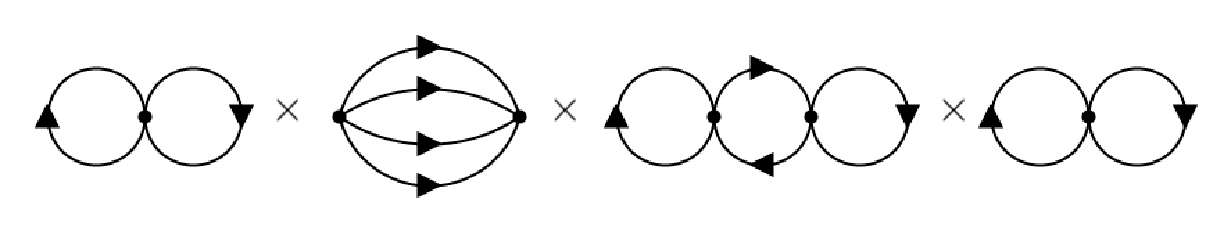
\includegraphics[width=0.60\textwidth, valign=c]{figurer/feynman-diagram/diagram_sum.pdf}
    \dots
\end{align}
%
If sub-diagram $i$ as a stand-alone diagram equals $\Em_i$, each copy of that subdiagram contributes a factor $\Em_i$ to the total diagram.
However, due to the symmetry of permuting identical subdiagrams, one must divide by the extra symmetry factor $s = n_i !$, the total number of permutations of all the copies of diagram $i$.
The full diagram therefore equals
%
\begin{align}
    \Em
    = \prod_{i= 1}^N \frac{1}{n_i!} \Em_i^{n_i}.
\end{align}
%
$\Em$ is uniquely defined by a finite sequence of integers, $(n_1, n_2, \dots n_N, 0, 0, \dots)$, so the sum of all diagrams is the sum over the set $S$ of all finite sequences of integers.
This allows us to write the sum of all diagrams as
%
\begin{equation}
    \label{sum of all diagrams}
    \sum_{(n_1, ...)\in S} \prod_{i} \frac{1}{n_i!} \Em_i^{n_i}
    = \prod_{i = 1}^{\infty} \sum_{n_i=1}^{\infty} \frac{1}{n_i!} \Em_i^{n_i}
    = \exp{{\sum}_i \Em_i}.
\end{equation}
%
We showed that the generating functional $Z[J]$ were the $Z_0[0]$ times the sum of all diagrams due to external sources.
From \autoref{sum of all diagrams}, if we define
%
\begin{equation}
    Z[J] = Z_0[0]\exp{i W[J]},
\end{equation}
%
then $W[J]$ is the sum of all connected diagrams. This is trivially true for the free theory, where the only connected diagram is
%
\begin{equation}
    \label{generating functional of connected diagrams}
    W_0[J] = J(x) \,\,
    \feynmandiagram [horizontal=a to b]{
        a [dot] -- [fermion] b [dot]
    };
    \,\,
    J(y).
\end{equation}
%
The two-point function in the full, interacting theory can thus be written
%
\begin{equation}
    -i \fdv{W[J]}{J(x),J(y)} = D(x - y).
\end{equation}


    \section{*The 1PI effective action}

\label{section: effective action}
This section is based on \autocite{peskinIntroductionQuantumField1995,schwartzQuantumFieldTheory2013,weinbergQuantumTheoryFields1995,weinbergQuantumTheoryFields1996}


The generating functional for connected diagrams, $W[J]$, is dependent on the external source current $J$.
We can define a new quantity with a different independent variable, using the Legendre transformation analogously to what is done in thermodynamics and Lagrangian mechanics.
The new independent variable is
\begin{equation}
    \varphi_J(x) := \frac{\delta W[J]}{\delta J(x)} = \ex{\varphi(x)}_J.
\end{equation}
%
The subscript $J$ on the expectation value indicate that it is evaluated in the presence of a source.
The Legendre transformation of $W$ is then
\begin{equation}
    \label{1PI effective action}
    \Gamma[\varphi_J]
    = W[J] - \int \dd^4 x \, J(x) \varphi_J(x).
\end{equation}
%
Using the definition of $\varphi_J$, we have that
\begin{equation}
    \label{effective equation of motion}
    \fdv{\Gamma[\varphi_J]}{\varphi_J(x)}
    = \int \dd^4 y \, \fdv{J(y)}{\varphi_J(x)} \fdv{J(y)} W[J]
    - \int \dd^4 y \, \fdv{J(y)}{\varphi_J(x)} \varphi_J(y)
    - J(x)
    = - J(x).
\end{equation}
%
If we compare this to the classical equations of motion of a field $\varphi$ with the action $S$,
\begin{equation}
    \frac{\delta S[\varphi]}{\delta \varphi(x)} = -J(x),
\end{equation}
%
we see that $\Gamma$ is an action that gives the equation of motion for the expectation value of the field, given a source current $J(x)$.

To interpret $\Gamma$ further, we observe what happens if we treat $\Gamma[\varphi]$ as a classical action with a coupling $g$.
The generating functional in this new theory is
\begin{equation}
    \label{partition function with g}
    Z[J, g] = \int \D \varphi \,
    \exp{ i g^{-1} \left( \Gamma[\varphi] + \int \dd^4x \, \varphi(x) J(x) \right) }
\end{equation}
%
The free propagator in this theory will be proportional to $g$, as it is given by the inverse of the equation of motion for the free theory.
All vertices in this theory, on the other hand, will be proportional to $g^{-1}$, as they are given by the higher-order terms in the action $g^{-1}\Gamma$.
This means that a diagram with $V$ vertices and $I$ internal lines is proportional to $g^{I-V}$.
Regardless of what the Feynman-diagrams in this theory are, the number of loops of a connected diagram is\footnote{This is a consequence of the Euler characteristic $\chi = V - E + F$.}
\begin{equation}
    \label{Number of loops}
    L = I - V + 1.
\end{equation}
%
To see this, we first observe that diagrams with one single loop must have equally many internal lines as vertices, so the formula holds for $L = 1$.
The formula still holds if we add a new loop to a diagram with $n$ loops by joining two vertices.
If we attach a new vertex with one line, the formula still holds, and as the diagram is connected, any more lines connecting the new vertex to the diagram will create additional loops.
This ensures that the formula holds by induction.
As a consequence of this, any diagram is proportional to $g^{L-1}$.
This means that in the limit $g \rightarrow 0$, the theory is fully described at the tree-level, i.e., by only considering diagrams without loops.
In this limit, we may use the stationary phase approximation, as described in \autoref{appendix: Functional derivatives}, which gives
\begin{equation}
    Z[J, g\rightarrow 0] \approx 
    C \det\left(- \fdv{ \Gamma[\varphi_J]}{\varphi(x), \varphi(y)}\right)\,
    \exp{i g^{-1} \left(\Gamma[\varphi_J] + \int \dd^4x \, J(x) \varphi_J(x) \right)  }.
\end{equation}
%
This means that
\begin{equation}
    -i g \ln(Z[J, g]) 
    = g W[J, g] 
    = \Gamma[\varphi_J] + \int \dd^4x\,  J(x) \varphi_J(x) + \mathcal{O}(g),
\end{equation}
%
which is exactly the Legendre transformation we started out with, modulo the factor $g$.
$\Gamma$ is, therefore, the action that describes the full theory at the tree level.
For a free theory, the classical action $S$ equals the effective action.

As we found in the last section, the propagator $D(x, y) = \ex{\varphi(x)\varphi(y)}_J$ is given by $-i$ times the second functional derivative of $W[J]$.
Using the chain rule, together with \autoref{effective equation of motion}, we get
%
\begin{align*}
    \label{Effective action inverse propagator}
    (-i)\int \dd^4 z \frac{\delta^2 W[J]}{\delta J(x) \delta J(z)} 
    \frac{\delta^2 \Gamma[\varphi_J]}{\delta \varphi_J(z) \varphi_J(y)}
    =
    (-i)\int \dd^4 z \frac{\delta \varphi_J[z]}{\delta J(x)}
    \frac{\delta^2 \Gamma[\varphi_J]}{\delta \varphi_J(z) \varphi_J(y)}
    =
    (-i)\fdv{}{J(x)}  \fdv{\Gamma[\varphi_J]}{\varphi_J(y)}
    = i\delta(x - y).
\end{align*}
%
This is exactly the definition of the inverse propagator,
%
\begin{equation}
    \fdv{\Gamma[\varphi_J]}{\varphi_J(x),\varphi_J(y)} = D^{-1}(x, y).
\end{equation}
%
The inverse propagator is the sum of all one-particle-irreducible (1PI) diagrams, with two external vertices.
More generally, $\Gamma$ is the generating functional for 1PI diagrams, which is why it is called the 1PI effective action.

$\Gamma$ may be viewed as an effective action as defined in the introduction.
We define $\eta$ as the fluctuations around the expectation value of the field, $\varphi(x) = \varphi_J(x) + \eta(x)$, and use this to change variables of integration in the path integral.
The expectation value $\varphi_J$ is constant with respect to the integral, so 
\begin{equation}
    \int \D \varphi \, \exp{i S[\varphi]}
    = \int \D \eta \, \exp{iS[\varphi_J + \eta]}.
\end{equation}
%
By assumption, $\ex{\eta}_J = 0$, which means this path integral is described by only 1PI diagrams, connected or not. We can therefore write
%
\begin{equation}
    \exp{i \Gamma[\varphi_J]} = \int \D \eta \, \exp{iS[\varphi_J + \eta]}.
\end{equation}
%
As we will discuss later, we interpret this form as \emph{integrating out} the $\eta$ degrees of freedom, leaving us with an effective description of the physics dependent only on the ground state solution $\varphi_J$.
The disadvantage of this is that there is no bound on how complicated $\Gamma$ might be---it is not restricted by the usual assumptions of the form of the action, such as locality~\autocite{schwartzQuantumFieldTheory2013}.
With some simplifying assumptions, though, we can still make use of the 1PI effective action, as we will see in the next subsection.




\subsection{Effective potential}

For a constant field configuration $\varphi(x) = \varphi_0$, the effective action, a functional, becomes a regular function.
We define the effective potential $\Veff$ by
%
\begin{equation}
    \label{definition effective potential}
    \Gamma[\varphi_0] = - V T \, \Ve_{\mathrm{eff}}(\varphi_0),
\end{equation}
%
where $VT$ is the volume of space-time.
For a constant ground state, the effective potential will equal the energy of this state.
To calculate the effective potential, we can expand the action around this state to calculate the effective action,
by changing variables to $\varphi(x) = \varphi_0 + \eta(x)$.
$\eta(x)$ now parametrizes fluctuations around the ground state, and has by assumption a vanishing expectation value.
The generating functional becomes
%
\begin{align}
    Z[J] 
    = \int \D (\varphi_0 + \eta) \, 
    \exp{i S[\varphi_0 + \eta] + i \int \dd^4 x\, [\varphi_0 + \eta(x)] J(x) }.
\end{align}

The functional version of a Taylor expansion, as described in \autoref{appendix: Functional derivatives}, is
%
\begin{equation}
    S[\varphi_0 + \eta] = 
    S[\varphi_0]
    + \int \dd x \, \eta(x) \, \fdv{S[\varphi_0]}{\varphi(x)}
    + \frac{1}{2} \int \dd x \dd y\,  \eta(x) \eta(y) \,
    \frac{\delta^2 S[\varphi_0]}{\delta\varphi(x)\delta\varphi(y)}
    + \dots
\end{equation}
%
The notation
%
\begin{equation}
    \fdv{S[\varphi_0]}{\varphi(x)}
\end{equation}
%
indicates that the functional $S[\varphi]$ is differentiated with respect to $\varphi(x)$, then evaluated at $\varphi(x) = \varphi_0$.
We define
%
\begin{align}
    S_0[\eta] &:= 
    \int \dd^4 x \dd^4 y \,\eta(x)\eta(y)\, 
    \fdv{S[\varphi_0]}{\varphi(x), \varphi(y)}, \\
    S_I[\eta] &:=
    \int \dd^4 x \dd^4 y \dd^4 z \,\eta(x)\eta(y)\eta(z)\, 
    \fdv{S[\varphi_0]}{\varphi(x),\varphi(y),\varphi(z)} + \dots,
\end{align}
%
where the dots indicate higher derivatives.
When we insert this expansion into the generating functional $Z[J]$ we get
%
\begin{align}
    &Z[J] = \int \D \eta \,
    \exp{
        i \int \dd^4 x \left(  \Ell[\varphi_0] + J \varphi_0  \right)
        +i \int \dd^4x \, \eta(x) \, 
        \left(  \fdv{S[\varphi_0]}{\varphi(x)} + J(x) \right)
        + i S_0[\eta] + i S_I[\eta]
    }.
\end{align}
%
The first term is constant with respect to $\eta$ and may be taken outside the path integral.
The second term gives rise to tadpole diagrams, which alter the expectation value of $\eta(x)$.
For $J=0$, this expectation value should vanish, and this term can be ignored.
Furthermore, this means that the ground state must minimize the classical potential,
\begin{equation}
    \label{minimize classical potential}
    \pdv{\Ve(\varphi_0)}{\varphi} = 0.
\end{equation}
%
%
This leaves us with 
%
\begin{equation}
    -i \ln Z[J] = W[J]
    =
    \int \dd^4 x \left(  \Ell[\varphi_0] + J \varphi_0  \right)
    -i \ln
    \left(
        \int \D \eta\exp{i S_0[\eta] + i S_I[\eta]}
    \right).
\end{equation}
%
%
We can now use the definition of the 1PI effective action to obtain a formula for the effective potential,
%
\begin{equation}
    \Veff(\varphi_0)
    =- \frac{1}{VT}
    \left( 
        W[J] - \int \dd^4 x \, J(x) \varphi_0
    \right)
    = \Ve(\varphi_0) 
    -i \ln
    \left(
        \int \D \eta\exp{i S_0[\eta] + i S_I[\eta]}
    \right).
\end{equation}
%

In \autoref{1PI effective action}, we showed that the 1PI effective action describes the whole quantum theory of the original action at the tree-level.
This was done by inspecting a theory with an action proportional to $g^{-1}$.
In this theory, Feynman diagrams with $L$ loops are proportional to $g^{L-1}$.
We can use the same argument to expand the effective potential in loops.
This is done by modifying the action $S[\varphi] \rightarrow g^{-1}S[\varphi]$, and then expand in power of $g$.
The first term in the effective potential is modified by $\Ve \rightarrow g^{-1}\Ve$, which means that it is made up of tree-level terms.
This is as expected, since the tree-level result corresponds to the classical result without any quantum corrections.
The second term becomes
%
\begin{align*}
    \ln
    \left(
        \int \D \eta \, e^{i S_0 + i S_I}
    \right)
    \longrightarrow
    &
    \ln
    \left(
        \int \D \eta \, e^{i g^{-1}S_0 + i g^{-1} S_I}
    \right)
    = 
    \ln\left(
        \int \D \eta \, e^{i g^{-1}S_0}
    \right)
    +
    \ln
    \left(
        \frac{
            \int \D \eta\, e^{i g^{-1} S_I} \, e^{i g^{-1}S_0}
        }{
            \int \D \eta\,e^{i g^{-1}S_0}
        }
    \right)
\end{align*}
%
The first term is quadratic in $\eta$, and can therefore be evaluated as a generalized Gaussian integral, as described in \autoref{appendix: Functional derivatives},
%
\begin{align*}
    & 
    \ln\Bigg[
        \int \D \eta \, 
    \exp{
            i g^{-1} \frac{1}{2} \int \dd^4x \dd^4y\,  \eta(x) \eta(y) \, 
            \fdv{S[\varphi_0]}{\varphi(x),\varphi(y)} 
    }
    \Bigg]
    \\
    & 
    = 
    \ln\Bigg[
        \det\left( - g^{-1} \fdv{S[\varphi_0]}{\varphi(x), \varphi(y)} \right)^{-1/2}
    \Bigg]
    = -\frac{1}{2}
    \Tr{
        \ln\left[
        - \fdv{S[\varphi_0]}{\varphi(x), \varphi(y)}
        \right]
    }
    + \const
\end{align*}
%
We then use the identity $\ln\{\det M \}= \Tr{\ln M}$.
After we remove the constant, this term is proportional to $g^0$, i.e., it is made up of one-loop terms.

The last term can be evaluated by first expanding the exponential containing the $S_I$ term, then using $\ln(1 + x) = \sum_n \frac{1}{n}x^n$.
Using
%
\begin{equation}
    \ex{A}_0 =  \frac{
        \int \D \varphi \, 
        A \, e^{ig^{-1}S_0}
    }{
        \int \D \varphi \, 
        e^{ig^{-1}S_0}
    },
\end{equation}
%
we can write
%
\begin{align}
    & \ln
    \left[
        \frac{
            \int \D \eta \, 
            e^{ig^{-1}S_I}e^{ig^{-1}S_0}
        }{
            \int \D \varphi \, 
            e^{ig^{-1}S_0}
        }
    \right]
    = 
    \ln 
    \left(
        \sum_{n = 0}^\infty \frac{1}{n!}
        \ex{(ig^{-1}S_I)^n}_0
    \right).
\end{align}
%
We recognize this as the sum of all connected Feynman diagrams, with Feynman rules from the interaction term $S_I$.
We know that $S_I$ is made up of terms that are third power or higher in the fields.
Each internal line is connected to two vertices, and each vertex is connected to at least three internal lines, i.e., $I \geq 3/2 V$.
The number of loops is therefore $L = I - V + 1 \geq (3/2 - 1)V + 1$.
There is at leas one vertex, i.e. $L \geq 3/2$.
This shows that the first logarithm contains \emph{all} one-loop contributions.
The effective potential to one-loop order is therefore
%
\begin{equation}
    \label{effective potential}
    \Veff(\varphi_0) = \Ve(\varphi_0) - \frac{i}{VT}  \frac{1}{2} \Tr{\ln\left( - \fdv{S[\varphi_0]}{\varphi(x), \varphi(y)}  \right)}.
\end{equation}
%


    \section{Symmetry and Goldstone's theorem*}
\label{section:symmetry}

This section is based on~\autocite{leeIntroductionSmoothManifolds2003d,peskinIntroductionQuantumField1995,schwartzQuantumFieldTheory2013,weinbergQuantumTheoryFields1995,weinbergQuantumTheoryFields1996}.

Symmetry plays a prominent role in modern physics.
If we can transform a physical state in such a way that the governing equations of this system are unchanged, we call that transformation a \emph{symmetry transformation}.
All such transformations are known as the symmetries of that theory.
The symmetries of a theory encode a lot of physics, such as the presence of conserved quantities and the system's low energy behavior.
We distinguish between internal and external symmetries.
An external symmetry is an active coordinate transformation, such as rotations or translations.
They relate degrees of freedom at different space-time points, while internal symmetries transform degrees of freedom at each space-time point independently.
A further distinction is between global and local symmetry transformations.
Global transformations have one rule for transforming degrees of freedom at each point, which is applied everywhere, while local transformations are functions of space-time.

In classical field theory, symmetries are encoded in the behavior of the Lagrangian when the fields are transformed.
We will consider continuous transformations, which can in general be written as
\begin{equation}
    \varphi(x) \longrightarrow \varphi'(x) = f_t[\varphi](x), \quad t \in [0, 1].
\end{equation}
%
Here, $f_t[\varphi]$ is a functional in $\varphi$, and a smooth function of $t$, with the constraint that $f_0[\varphi] = \varphi$.
This allows us to look at ``infinitesimal'' transformations,
\begin{equation}
    \label{infinitesimal transformation}
    \varphi'(x) = f_\epsilon[\varphi] 
    = \varphi(x) + \epsilon \odv{ f_t[\varphi] }{t}\bigg |_{t=0} + \Oh{\epsilon}.
\end{equation}
%
When considering infinitesimal transformations, we will not always write $ + \Oh{\epsilon}$, but rather consider it implicit.
We will consider internal, global transformations which act linearly on $\varphi$.
For $N$ fields, $\varphi_i$, this can be written
\begin{equation}
    \label{linear field transformation}
    \varphi_i'(x) = \varphi_i(x) + \epsilon \, i V_{ij} \varphi_j(x).
\end{equation}
%
$V_{ij}$ is called the generator of the transformation.
A symmetry transformation of the system is then a transformation in which the Lagrangian left is unchanged, or at most differ by a 4-divergence term.
That is, a transformation $\varphi \rightarrow \varphi'$ is a symmetry if 
\begin{equation}
    \Ell[\varphi'] = \Ell[\varphi] + \partial_\mu K^\mu[\varphi],
\end{equation}
%
where $K^\mu[\varphi]$ is a functional of $\varphi$.\footnote{Terms of the form $\partial_\mu K^\mu$ does not affect the physics, as variational principle $\delta S = 0$ do not vary the fields at infinity. Together with the divergence theorem, this means that such terms do not influence the equations of motion.}
This is a requirement for symmetry in quantum field theory too.
However, as physical quantities in quantum field theory are given not just by the action of a single state but the path integral, the integration measure $\D \varphi$ has to be invariant as well.
If a classical symmetry fails due to the non-invariance of the integration measure, it is called an \emph{anomaly}.

To investigate the symmetry properties of a quantum theory, we explore what constraints a symmetry imposes on the effective action.
To that end, assume 
\begin{equation}
    \D \varphi'(x) = \D \varphi(x), \quad
    S[\varphi'] = S[\varphi].
\end{equation}
%
In the generating functional, such a transformation corresponds to a change of integration variable.
Using the infinitesimal version of the transformation, we may write
\begin{align}
    \nonumber
    Z[J]
    = \int \D \varphi \, \exp{i S[\varphi] + i \int \dd^4 x \,J_i(x) \varphi_i(x)} 
    = \int \D \varphi' \, \exp{i S[\varphi'] + i \int \dd^4 x \, J_i(x) \varphi'_i(x)}
    \\
    = Z[J] + i \epsilon \int \dd^4 x \, J_i(x) \int \D \varphi \, [V_{ij} \varphi_j(x)]  e^{i S[\varphi]},
\end{align}
%
Using \autoref{effective equation of motion}, we can write this as
\begin{equation}
    \label{effective action symmetry requirement}
    \int \dd^4 x \, \fdv{\Gamma[\varphi_J]}{\varphi_i(x)} \, V_{ij}\ex{\varphi_j(x)}_J = 0.
\end{equation}
%
This constraint will allow us to deduce the properties of a theory close to the ground state, only using information about the symmetries of the theory.


The archetypical example of an internal, global, and continuous symmetry is the linear sigma model, which we will use as an example throughout this section.
The linear sigma model is made up of $N$ real scalar fields $\varphi_i$, whose Lagrangian is
\begin{equation}
    \Ell[\varphi] 
    = \frac{1}{2} \partial_\mu \varphi_i(x) \partial^\mu \varphi_i(x) - \Ve(\varphi),
    \quad \Ve(\varphi) = - \frac{1}{2} \mu^2 \varphi_i(x)\varphi_i(x)
    + \frac{1}{4} \lambda [\varphi_i(x) \varphi_i(x)]^2.
\end{equation}
%
This system is invariant under the rotation of the $N$ fields into each other,
\begin{equation}
    \varphi_i \longrightarrow \varphi_i' = M_{ij} \varphi_j,
    \quad M^{-1} = M^{T}.
\end{equation}
%
The set of all such transformations forms the Lie group $\text{O}(N)$.
Lie groups will be discussed in the next section.
For $N = 2$, and $\mu^2, \lambda > 0$ we get the ubiquitous Mexican hat potential, as illustrated in \autoref{fig:Mexican hat}.

\begin{figure}[ht]
    \centering
    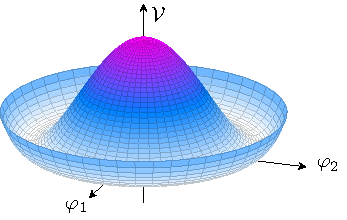
\includegraphics[width=0.6\textwidth]{figurer/mexican_hat.pdf}
    \caption{The Mexican hat potential is the classical potential $\Ve$ for the $N=2 $ linear sigma model.}
    \label{fig:Mexican hat}
\end{figure}

\subsection{Nöther's theorem}

One of the most profound consequences of symmetry in physics is the appearance of conserved quantities.
Assume we have a set of fields $\varphi_i$. Nöther's theorem tells us that if the Lagrangian $\Ell[\varphi_i]$ has a continuous symmetry, then there is a corresponding conserved current~\autocite{carrollSpacetimeGeometryIntroduction2019,peskinIntroductionQuantumField1995}.
Consider an infinitesimal transformation,
\begin{equation}
    \varphi_i(x) \longrightarrow \varphi_i'(x)
    = \varphi_i(x) + \delta \varphi_i(x),.
\end{equation}
%
Applying this transformation to the Lagrangian will in general change its form,
\begin{equation}
    \Ell[\varphi] \rightarrow \Ell[\varphi']
    = \Ell[\varphi] + \delta \Ell.
\end{equation}
%
We assume this transformation is a symmetry, i.e.,
\begin{equation*}
    \delta \Ell = \partial_\mu K^\mu.
\end{equation*}
%
By considering the Lagrangian as a function of the field and its derivatives, $\Ell = \Ell(\varphi_i, \partial_\mu \varphi_i)$, we can write the difference term as a Taylor expansion around $(\varphi_i, \partial_\mu \varphi_i)$,
\begin{align}
    \delta \Ell
    = \pdv{\Ell}{\varphi_i} \delta \varphi_i
    + \pdv{\Ell}{(\partial_\mu \varphi_i)} \delta (\partial_\mu \varphi_i),
\end{align}
%
where $\delta (\partial_\mu \varphi_i) = \partial_\mu \varphi_i' - \partial_\mu \varphi_i$.
By the linearlity of the derivative,
\begin{equation}
    \delta (\partial_\mu \varphi_i)
    = \partial_\mu \varphi_i' - \partial_\mu \varphi_i
    = \partial_\mu (\varphi_i' - \varphi_i)
    = \partial_\mu \delta \varphi_i.
\end{equation}
%
With this, and the Euler-Lagrange equations
\begin{equation}
    \partial_\mu \pdv{\Ell}{(\partial_\mu \varphi)} - \pdv{\Ell}{\varphi_i} = 0,
\end{equation}
%
we can rewrite
\begin{equation}
    \delta \Ell = \left( \partial_\mu \pdv{\Ell}{(\partial_\mu \varphi_i)} \right) \delta \varphi_i
    + \pdv{\Ell}{(\partial_\mu \varphi_i)} (\partial_\mu \delta \varphi_i)
    = \partial_\mu \left(\pdv{\Ell}{(\partial_\mu \varphi_i)} \delta \varphi_i\right)
\end{equation}
%
If we define the current
\begin{equation}
    j^\mu = \pdv{\Ell}{(\partial_\mu \varphi_i)} \delta \varphi_i(x) - K^\mu,
\end{equation}
%
then 
\begin{equation}
    \partial_\mu j^\mu = \delta \Ell - \delta \Ell = 0.
\end{equation}
%
This is Nöther's theorem; a continuous symmetry implies the existence of a conserved current.

The current flux through some spacelike surface $V$ defines a conserved charge. The surface of constant time in some reference frame has the normal vector $n_\mu = (1, 0, 0, 0)$, so the charge is
\begin{equation}
    Q = \int_V \dd^4 x \, n_\mu j^\nu = \int_V \dd^3 x \, j^0.
\end{equation}
%
We can then use the divergence theorem.
Assume $\partial V$ is the boundary of $V$, which has the space-like normal vector $k_i$, and that the current falls of quickly towards infinity.
Then
\begin{equation}
    \odv{Q}{t} = - \int_V \dd^3 x \, \partial_i j^i = - \int_{\partial V} \dd^2 x\, k_i j^i = 0,
\end{equation}
%
proving that the charge is conserved.

\subsection{Goldstone's theorem}

A symmetry transformation will leave the governing equation of a theory unchanged.
This, however, does not imply that physical states, such as the ground state, are invariant under this transformation.
The $N = 2$ linear sigma model illustrates this.
If we assume the ground state $\varphi_{0}$ is translationally invariant, then it is given by minimizing the effective potential, of which the classical potential, $\Ve$, is the leading order approximation.
This potential is illustrated in \autoref{fig:Mexican hat}.
The ground state is therefore given by any of the values along the brim of the potential.
If we, without loss of generality, choose $\varphi_0 = (0, v)$ as the ground state, then any rotation will change this state.
We say that the symmetry has been \emph{spontaneously broken}.

To explore this in a general context, assume a theory of $N$ real scalar fields $\varphi_i$ are invariant under the actions of some Lie group, $G$.
A symmetry $g \in G$ is broken if the vacuum expectation value of the original fields and the transformed fields differ.
That is, if
\begin{equation}
    \ex{\varphi}_0 \neq \ex{\varphi'}_0 = \ex{g \varphi}_0
\end{equation}
%
We can now exploit what we learned about Lie groups to write the infinitesimal transformation as
\begin{equation}
    \ex{\varphi'}_0 = \ex{\varphi}_0 + i \epsilon \eta_\alpha T_\alpha \ex{\varphi}_0.
\end{equation}
%
Let $x_i$ be the set of generators corresponding to broken symmetries, i.e.,
\begin{equation}
    x_i \ex{\varphi}_0 \neq 0.
\end{equation}
%
These are called the \emph{broken generators}.
The remaining set of generators $t_a$, which obey
\begin{equation}
    t_a \ex{\varphi}_0 = 0,
\end{equation}
%
are called unbroken, and generate a subgroup $H \subset G$ as the set of symmetry transformations of the vacuum is a group.

In \autoref{effective action symmetry requirement} we found that, if $V$ is the generator of some symmetry, then the effective action obeys
\begin{equation}
    \int \dd^4 x\, \fdv{\Gamma[\varphi_J]}{\varphi_i} V_{ij} \ex{\varphi_j}_0 = 0,
\end{equation}
%
We now differentiate this expression with respect to $\varphi_k(y)$ and evaluate it in the vacuum, which gives
\begin{equation}
    \int \dd^4 x \, \fdv{\Gamma[\varphi_0]}{\varphi_k(y), \varphi_i(x)}
    V_{ij} \ex{\varphi_j}_0 = 0.
\end{equation}
%
With the assumption that the ground state is constant, we get 
\begin{equation}
    \pdv{\Veff}{\varphi_k, \varphi_i} \, V_{i j} \ex{\varphi_j}_0 = 0.
\end{equation}
%
This is trival for unbroken symmetries, as $t^a_{ij}\ex{\varphi_j}_0 = 0$ by definition.
However, in the case of a broken symmetry, the second derivative of the effective potential has an eigenvector $x^\ell_{ij} \ex{\varphi_j}_0$ with a zero eigenvalue for each broken generator.
Here, $\ell$ label the set of generators, while $(ij)$ are the indices corresponding to field-components $\varphi_i$.
In \autoref{Effective action inverse propagator}, we found that the second derivative of the effective action is the inverse propagator,
\begin{equation}
    D^{-1}_{ij}(x,y) 
    = \fdv{\Gamma[\varphi_0]}{\varphi_i(y), \varphi_j(x)}
    = \int \frac{\dd^4 p}{(2 \pi)^4} e^{-ip(x - y)} \, \tilde D^{-1}_{ij}(p).
\end{equation}
%
Using this, we can write
\begin{equation}
    \tilde D^{-1}_{i j}(p=0) \, x^\ell_{jk} \ex{\varphi_k}_0 
    = 0.
\end{equation}
%
Zeros of the inverse propagator correspond to the physical mass of particles.
In Lorentz-invariant systems, each zero-eigenvalue vector corresponds to a masses particle, called a Goldstone boson.\footnote{ The particles are bosons due to the bosonic nature of the transformations, $g$. If the generators are Grassmann numbers, the resulting particles, called goldstinos, are fermions.}
This means there are $n_G = \dim G -\dim H$ zero-mass modes.
In general, the counting of massless modes is complicated and depends on the dispersion relation of the particles at low momenta.
Systems with Goldstone bosons with quadratic dispersion relation, that is $E \propto |\vv p|^2$ when $\vv p \rightarrow 0$, often exhibit a lower number of massless modes.
An example is ferromagnets, where the $\mathrm{SU}(2)$ rotational symmetry is broken down to $\mathrm{U}(1)$ when they align along one axis. 
This corresponds to two broken generators, yet the system exhibits only one massless mode~\autocite{braunerSpontaneousSymmetryBreaking2010}.

\begin{figure}[ht]
    \centering
    \hspace*{2.5cm}
    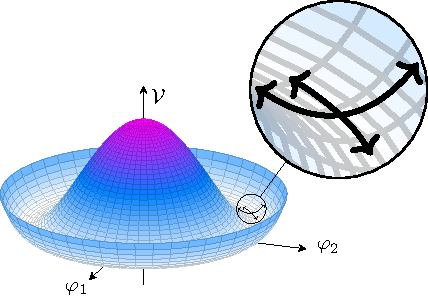
\includegraphics[width=.6\linewidth]{figurer/mexican_hat_zoom.pdf}
    \caption{Excitations along the brim does not cost any energy, as the potential is flat, unlike excitations in the radial direction.}
    \label{fig:Mexican hat zoom}
\end{figure}

The linear sigma model gives an intuition for the Goldstone mode.
In the case of $N = 2$, the symmetry of the Lagrangian are rotations in the plane.
As the ground state is a point along the ``brim'' of the hat, this rotational symmetry is broken.
However, any excitations in the angular direction do not cost any energy, which is indicative of a massless mode.
This is illustrated in \autoref{fig:Mexican hat zoom}.
In this example, the original symmetry group is one-dimensional, so there are no unbroken symmetries.
Consider instead the $N=3$ linear sigma model, which has the three-dimensional symmetry group $\SO(3)$, rotations of the sphere.
We see that the ground state is left invariant under a subgroup of the original symmetry transformations.
The ground state manifold of this system, the set of all states that minimizes the effective potential, is then a sphere.
When the system chooses one single ground state, this symmetry is broken, but only for two of the generators. 
The generator for rotations around the ground state leaves that point unchanged and is thus an unbroken symmetry.
Any excitations in the direction of the broken symmetries do not cost energy, as it is in the ground state manifold.
On the other hand, the unbroken symmetry does not correspond to an excitation.
This is illustrated in \autoref{fig:ground state manifold}.

\begin{figure}[h]
    \centering
    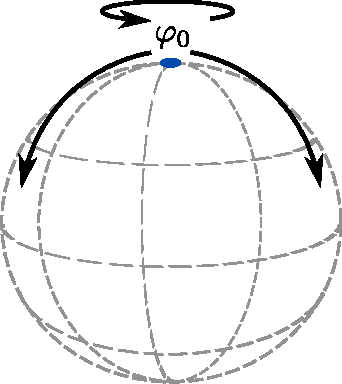
\includegraphics[width=.35\linewidth]{figurer/SU(3).pdf}
    \caption{Excitations for the $N=3$ sigma model. Two of the symmetries are broken, while rotations around the groundstate leaves the system unchanged.}
    \label{fig:ground state manifold}
\end{figure}

    \section{CCWZ construction*}
\label{seciton:ccwz construction}

As Goldstone bosons are massless, they play a crucial role in low-energy dynamics.
To best describe this limit, we seek a parametrization of the theory in which they are the degrees of freedom.
This can be done using the CCWZ construction, named after Callan, Coleman, Wess, and Zumino.
This section is based on~\autocite{morrisonColemanCallanWessZuminoConstruction2017,panicoCompositeNambuGoldstoneHiggs2016,weinbergQuantumTheoryFields1996,pichEffectiveFieldTheory2020}, as well as the original papers~\autocite{callanStructurePhenomenologicalLagrangians1969,colemanStructurePhenomenologicalLagrangians1969}.


We saw that the Goldstone bosons correspond to excitations within the vacuum manifold.
The vacuum manifold corresponds to points in field space $\varphi$ that can be reached from the vacuum $\varphi_0$ with a transformation $g \in G$.
Assume this group acts linearly on the fields.
This means that we can write such excitations as
\begin{equation}
    \varphi_i = (\tilde\Sigma \varphi_0)_{i} = \tilde \Sigma_{ij} (\varphi_0)_j, 
    \quad \tilde \Sigma = \tilde \Sigma(\eta) = \exp{i \eta_\alpha T_\alpha}
\end{equation}
%
We will drop the indices for the sake of compact notation.
$\tilde \Sigma$ is thus a function from the parameter space, $\eta_\alpha \in \R^n$, to $G$,
\begin{align}
    \tilde \Sigma: \R^n \longmapsto G.
\end{align}
%
We then get space-time-dependent field configurations by making the parameters dependent on space-time.
We will for now assume $\eta_\alpha$ is constant.
This parametrization is highly redundant.
Two elements $\tilde\Sigma$ and $\tilde\Sigma'$, related by
\begin{equation}
    \tilde \Sigma' = \tilde\Sigma e^{i \theta_a t_a}
\end{equation}
%
results in the same $\varphi$.
This is because  $e^{i \theta_a t_a} = h \in H$, and $h \varphi_0 = \varphi_0$, by assumption.
The set of all equivalent $\tilde \Sigma$'s is exactly the left coset, $gH = \setbuilder{gh}{ h \in H}$.
The set of cosets forms a new manifold, $G / H$, called the Goldstone manifold.
This is a manifold of dimension $\dim(G/H) = \dim(G) - \dim(H)$, which is the number of broken generators and thus also the number of Goldstone modes.
Membership of a certain coset form an equivalence relation, $g \sim g'$ if $g' = gh$.
This means that the cosets $gH$ form a partition of $G$ and that each element $g \in G$ belongs to one, and only one, coset.
To remove the redundancy in the parametrization, we need to choose one representative element from each coset.

By the inverse function theorem, any mapping between manifolds $f: \Em \mapsto \mathcal{N}$ that has a non-degenerate differential, that is an invertible Jacobian, at a point $p \in \Em$, is invertible in a neighborhood of $p$.
If we write
\begin{equation}
    \tilde \Sigma(\xi, \theta) = \exp{i \xi_i x_i} \exp{i \theta_a t_a},
\end{equation}
%
then the map is invertible at $p = (\xi_i = 0, \theta_a = 0)$, as the Jacobian is the identity matrix.
This point is mapped to the identity element of $G$.
This means that, in a neighborhood $U \subset G$ of the identity, each element $g$ has a unique representation $g = \tilde \Sigma$~\autocite{leeSmoothManifolds2012}.
Furthermore, two elements $\tilde \Sigma'$ and $\tilde \Sigma$ related by $\tilde \Sigma' = \tilde \Sigma h$, $h \in H$ have the same $\xi$-arguments.
We see that $\xi_i$ parametrize $G/H$, in the neighborhood of the identity.
We therefore demand that $\tilde \Sigma$ always appear in the standard form
\begin{equation}
    \Sigma(\xi) = \tilde \Sigma(\xi, 0) = \exp{i \xi_i x_i}.
\end{equation}
%
The field $\varphi(x)$ can therefore be written as
\begin{equation}
    \varphi(x) = \Sigma(x) \varphi_0 = \exp{i \xi_i(x) x_i} \varphi_0,
\end{equation}
%
and $\xi_i(x)$ can be associated with the Goldstone bosons.

In the linear sigma model, the original $\Olie(N)$ symmetry is broken down to $\Olie(N-1)$, which transforms the remaining $N-1$ fields with vanishing expectation values into each other.
However, $\Olie(N)$ consists of two disconnected subsets, those matrices with determinant 1 and those with determinant -1.
There is no continuous path that takes an element of $\Olie(N)$ with determinant of $-1$ to an element with determinant 1.\footnote{A simple proof of this is the fact that the determinant is a continuous function, while any path $\det M(t)$ such that $\det M(1) = -1,\, \det M(0) = 1$ must make a discontinuous jump.}
The set of symmetries that are connected to the identity is
\begin{eqnarray}
    G = SO(N) = \setbuilder{M \in \Olie(N)}{ \det M = 1}.
\end{eqnarray}
If we choose $\varphi_0 = (0, 0, ..., v)$, then it is apparent that the ground state is invariant under the rotations of the $N-1$ first fields, so the unbroken symmetry is  $H = \SO(N-1)$.
The Goldstone manifold is $G/H = \SO(N) / \SO(N-1)$.

Consider the case of $N = 3$, which is illustrated in \autoref{fig:ground state manifold}.
$G$ is the rotations of the sphere, while $H$ is rotations around $\varphi_0$, $\SO(2)$.
The Goldstone manifold consists of the rotations of $\varphi_0$ to other points of the sphere, i.e. $G/H = \SO(3)/\SO(2) = S^2$, the 2-sphere.
This is not a Lie group, as translating $\varphi$ in a closed path around the sphere may result in a rotation around the z-axis.
This is illustrated in \autoref{fig:Curvature of SO(3)}


To check that $\xi_i$, in fact, are the Goldstone modes, we study the way they appear in the Lagrangian.
As they are massless, no mass term of the form $M_{ij} \xi_i \xi_j$ should appear.
The original Lagrangian $\Ell[\varphi]$ was invariant under global transformations $\varphi(x) \mapsto g \varphi(x)$.
However, any terms that only depend on $\varphi(x)$, and not its derivatives, will also be invariant under a \emph{local} transformation, $\varphi(x) \mapsto g(x)\varphi(x)$.
Our parametrization of the fields, $\varphi(x) = \Sigma(x)\varphi_0$ is exactly such a transformation, which means that any such terms are independent of the Goldstone bosons.
We can therefore write
\begin{equation}
    \Ell[\varphi] = \Ell_{\mathrm{kin}}[\varphi] + V(\varphi_0),
\end{equation}
%
where all terms in $\Ell_{\mathrm{kin}}$ are proportional to at least one derivative term, $\partial_\mu \varphi(x)$.
Inserting the parametrization into this derivative term, we get
\begin{equation}
    \partial_\mu \varphi(x) = \partial_\mu [\Sigma(x) \varphi_0]
    = \Sigma(x) [\Sigma(x)^{-1} \partial_{\mu} \Sigma(x)] \varphi_0.
\end{equation}
%
The Lagrangian will therefore depend on $\xi_i$ via terms of the form $\Sigma(x)^{-1}\partial_\mu \Sigma(x)$, which is called the Mauer-Cartan form.
This is a $\mathfrak g$-valued function, which means that it can be written as
\begin{align}
    i\Sigma(x)^{-1}\partial_\mu \Sigma(x) & 
    = d_{\mu}(x) + e_{\mu}(x), \\
    d_{\mu} & = i x_i d_{ij}(\xi) \partial_\mu \xi_j, \\
    e_{\mu} & = i t_a e_{ai}(\xi)\partial_\mu \xi_i,
\end{align}
%
where $d_{ij}$ and $e_{ai}$ are as-of-yet unknown real valued functions of $\xi$~\autocite{watanabeEffectiveLagrangianNonrelativistic2014,weinbergQuantumTheoryFields1996}.

\subsection{Transformation properties of Goldstone bosons}
We can deduce how the Goldstone bosons transforms under $G$ from how $\varphi$ transforms.
In general, 
\begin{equation}
    \varphi' = g \varphi = (g \Sigma(\xi)) \varphi_0 = \Sigma(\xi') \varphi_0 \quad g \in G.
\end{equation}
%
While $\Sigma(\xi')$ has the standard form by assumption,
\begin{equation}
    \Sigma(\xi') = \exp{i \xi'_i x_i},
\end{equation}
%
$g\Sigma(\xi)$ does not, in general.

\begin{figure}[h]
    \centering
    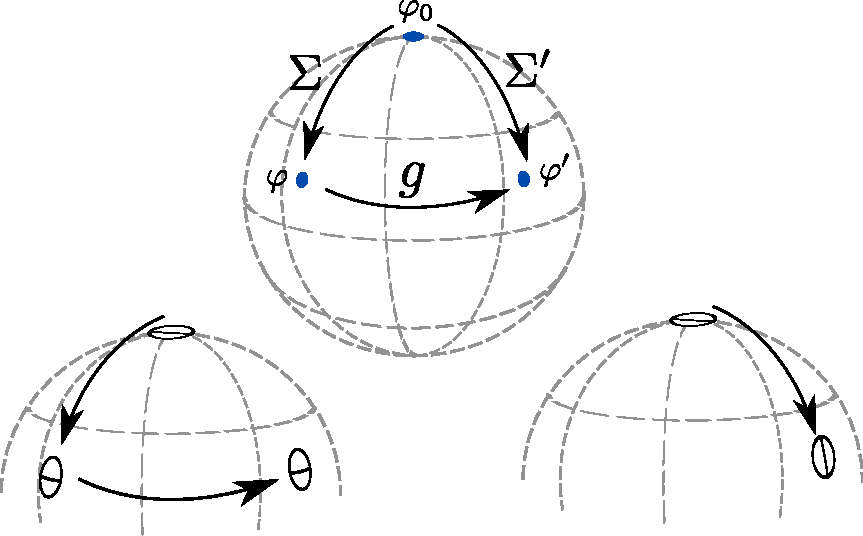
\includegraphics[width=0.8\textwidth]{figurer/curvature.pdf}
    \caption{The top figure illustrates the transformation of $\varphi_0$ to $\varphi$ and then $\varphi'$, and the alternative, direct transformation $\varphi_0 \rightarrow \varphi'$. The bottom figure illustrates how this can rotate a neighborhood of $\varphi_0$ differently.}
    \label{fig:Curvature of SO(3)}
\end{figure}
\autoref{fig:Curvature of SO(3)} illustrates this in the case of $G = \SO(3)$.
$\Sigma(\xi)$ transforms $\varphi_0$ to $\varphi$, then $g$ transforms $\varphi$ to $\varphi' = \Sigma(\xi') \varphi_0$.
Assuming $\varphi$ and $\varphi'$ are close enough to $\varphi_0$, we can write $\Sigma(\xi)$ and $\Sigma(\xi')$ on the standard form.
However, if we follow a small neighborhood around $\varphi_0$ as it is acted on by $\Sigma(\xi)$, then $g$, it will be rotated by the time it arrives at $\varphi'$ when compared to the same neighborhood if it was acted on by $\Sigma(\xi')$.

$g\Sigma(\xi)$ and $\Sigma(\xi')$ are in the same coset, as they by assumption corresponds to the same physical state.
This means that we can write $g\Sigma(\xi) = \Sigma(\xi') h(g, \xi)$, where $h(g, \xi) \in H$.
The transformation rule of $\xi$ under $G$ is therefore implicitly defined by
\begin{equation}
    \Sigma(\xi') = g \Sigma(\xi) [h(g, \xi)]^{-1}.
\end{equation}
%
This is, in general, not a linear representation, which is why this construction also is called a \emph{non-linear realization}.
Using the transformation rule, we can obtain the transformation rule of the Maurer-Cartan form.
We use the shorthand $\Sigma = \Sigma(\xi),\, \Sigma' = \Sigma(\xi')$, and $h = h(g, \xi)$.
This gives
\begin{align*}
    \Sigma^{-1} \partial_\mu \Sigma
    \rightarrow 
    & \, \Sigma'^{-1} \partial_\mu \Sigma' \\
    & = (g \Sigma h^{-1})^{-1} \partial_\mu (g \Sigma h^{-1}) \\
    & = (h \Sigma^{-1} g^{-1}) g [(\partial_\mu \Sigma)h^{-1} + \Sigma \partial_\mu h^{-1}] \\
    & = h \Sigma^{-1} (\partial_\mu \Sigma) h^{-1}
    + h \partial_\mu h^{-1} \\
    & = h (\Sigma^{-1} \partial_\mu \Sigma + \partial_\mu) h^{-1}.
\end{align*}
In terms of $d_\mu$ and $e_\mu$,
\begin{align}
    d_\mu & \rightarrow h d_\mu h^{-1} \\
    e_\mu & \rightarrow h (e_\mu + i\partial_\mu )h^{-1}.
\end{align}
%
These are our building blocks for constructing a general, $G$-invariant effective Lagrangian.
The trace of a product of $d_\mu$'s are invariant under $G$,
\begin{equation}
    \Tr{d_\mu d_\nu \dots d_\rho} 
    \rightarrow
    \Tr{h d_\mu h^{-1} h d_\nu h^{-1} h \dots d_\rho h^{-1}}
    = \Tr{d_\mu d_\nu \dots d_\rho},
\end{equation}
%
where we have used the cyclic property of trace.
However, the terms must also obey the other symmetries of the Lagrangian, such as C or P-parity and Lorentz invariance.
The last criterion excludes any terms with free space-time indices.
In \todo{Legg til dette}{section:chiral pertubation theory}, we will construct an effective Lagrangian in powers of $d$.
The lowest order terms are therefore
\begin{equation}
    \label{first order terms CCWZ}
    \Tr{d_\mu} \Tr{d^\mu}, 
    \quad 
    \Tr{d_\mu d^\mu}.
\end{equation}
%
We see that $e_\mu$ transforms like a gauge field, with the gauge group $H$.
If we include massive degrees of freedom and not only the Goldtone modes, $e_\mu$ is used to create a covariant derivative of the massive modes.
We are only interested in the Goldstone modes and will therefore be satisfied with $d_\mu$.
With these tools, we can create an effective theory of quantum chromodynamics at low energies.



    \chapter{General relativity and the TOV equation}
    \label{chapter: GR}
    (Newtonian gravity??)
\todo{Short about newtonian gravity/motivation}

\section{General relativity}
This section is based on~\cite{carrollSpacetimeGeometryIntroduction2019}.
The derivation of the spherically symmetric metric is done using computer code, as descirbed in \autoref{appendix: code}.

\subsection{Einstein's field equations}

General relativity describes spacetime as a smooth manifold $\Em$, with a (pseudo-Riemannian) metric, $g_{\mu \nu}$.
This metric is treated as a dynamical field, which is affected by the presence of matter and energy.
The matter and energy contents of spacetime are encoded in the stress-energy tensor $T_{\mu \nu}$, while the behavior of $g^{\mu \nu}$ is encoded in a scalar Lagrangian density.
Some of the mathematics used in this section, such as functional derivatives, are covered in \autoref{appendix: Functional derivatives}.

The most obvious---and correct---choice as the Lagrangian for $g^{\mu \nu}$ is the Ricci scalar, which results in the Einstein-Hilbert action,
%
\begin{equation}
    \label{Einstein-Hilbert action}
    S_{\text{EH}} = \frac{1}{2\kappa}\int_{\Em} \dd^n x \, \sqrt{|g|}\, R.
\end{equation}
%
The $\sqrt{|g|}$-factor is included for the integral to be coordinate-independent, as discussed in  \autoref{subsection: integration on manifolds}.\footnote{The gravitational action can also include a cosmological constant, modifying the Lagrangian to $R + 2 \Lambda$. This constant does not affect the subject of this thesis and is therefore not included here.}
The $\kappa$ is a constant and decides how strong the coupling of gravity to matter and energy is.
This constant can then be related to Newton's constant of gravitation $G$ by $\kappa = 8 \pi G$.
When including the contributions from other fields with an action $S_\text{m}$, the total action becomes 
%
\begin{equation}
    S = S_\text{EH} + S_\text{m}.
\end{equation}
%
The equations of motion of the dynamical field, which in this case is the metric, are given by Hamilton's principle of stationary action.
Using functional derivatives, as defined in \autoref{subsection: functional calculus on a curved manifold}, this is stated as
%
\begin{equation}
    \fdv{S}{g^{\mu\nu}} = 0,
\end{equation}
%
We define the stress-energy tensor as
%
\begin{equation}
    \label{definition stress energy densor}
    T_{\mu\nu} = - \frac{2}{\sqrt{|g|}} \fdv{S_\text{m}}{g^{\mu \nu}}.
\end{equation}
%
The functional derivative of the Einstein-Hilbert action is evaluated in \autoref{subsection: functional derivative of the einstein-hilbert action}, and with the result, \autoref{functional derivatie einstein-hilber action}, we get the Einstein field equations
%
\begin{equation}
    \label{Einstein field equations}
    R_{\mu \nu} - \frac{1}{2} R g_{\mu \nu} = \kappa T_{\mu \nu},
\end{equation}
%
The left-hand side of the Einstein field equations is called the Einstein tensor, $G_{\mu \nu} = R_{\mu \nu} - \frac{1}{2} R g_{\mu \nu}$. This tensor obeys the identity
\begin{equation}
    \label{Einstein tensor bianchi identity}
    \nabla^\mu G_{\mu \nu} = 0,
\end{equation}
as a consequence of the more general Bianchi identity.
\todo{Si hva bianchi identity er}


\subsection{Spherically symmetric spacetime}

To model stars, we will assume that the metric is spherically symmetric and time-independent.
In this case, the most general metric can be written, at least locally, as~\autocite{carrollSpacetimeGeometryIntroduction2019}
%
\begin{equation}
    \dd s^2 
    = e^{2\alpha(r)} \dd t^2 - e^{2 \beta(r)} \dd r^2 - 
    r^2 (\dd \theta^2 + \sin^2 \theta \, \dd \varphi^2),
\end{equation}
%
where $\alpha$ and $\beta$ are general functions of the radial coordinate $r$.
In matrix form, this corresponds to 
%
\begin{equation}
    \label{spherically symmetric metric}
    g_{\mu \nu} =
    \left(
        \begin{matrix}
            e^{2 \alpha{\left(r \right)}} & 0 & 0 & 0\\
            0 & - e^{2 \beta{\left(r \right)}} & 0 & 0
            \\0 & 0 & - r^{2} & 0
            \\0 & 0 & 0 & - r^{2} \sin^{2}{\left(\theta \right)}
        \end{matrix}
     \right).
\end{equation}
%
Using \autoref{christoffel symbols from metric}, we can now compute the Christoffel symbols in terms of the unknown functions.
These computations in this subsection are done using computer code, which is shown in \autoref{appendix: code}.
The results are
%
\begin{align}
    \Gamma^t_{\mu \nu}
    & =
    \left(
        \begin{matrix}
            0 & \frac{d}{d r} \alpha{\left(r \right)} & 0 & 0\\\frac{d}{d r} \alpha{\left(r \right)} & 0 & 0 & 0\\0 & 0 & 0 & 0\\0 & 0 & 0 & 0
        \end{matrix}
    \right), \\
    \Gamma^r_{\mu \nu}
    &=
    \left(
        \begin{matrix}
            e^{2 \alpha{\left(r \right)}} e^{- 2 \beta{\left(r \right)}} \frac{d}{d r} \alpha{\left(r \right)} & 0 & 0 & 0\\0 & \frac{d}{d r} \beta{\left(r \right)} & 0 & 0\\0 & 0 & - r e^{- 2 \beta{\left(r \right)}} & 0\\0 & 0 & 0 & - r e^{- 2 \beta{\left(r \right)}} \sin^{2}{\left(\theta \right)}
        \end{matrix}
     \right), \\
     \Gamma^\theta_{\mu \nu} 
     & =
     \left(
         \begin{matrix}
            0 & 0 & 0 & 0\\0 & 0 & \frac{1}{r} & 0\\0 & \frac{1}{r} & 0 & 0\\0 & 0 & 0 & - \sin{\left(\theta \right)} \cos{\left(\theta \right)}
        \end{matrix}
    \right), \\
    \Gamma^\phi_{\mu \nu} 
    &=
    \left(
        \begin{matrix}
            0 & 0 & 0 & 0\\0 & 0 & 0 & \frac{1}{r}\\0 & 0 & 0 & \frac{\cos{\left(\theta \right)}}{\sin{\left(\theta \right)}}\\0 & \frac{1}{r} & \frac{\cos{\left(\theta \right)}}{\sin{\left(\theta \right)}} & 0
        \end{matrix}
    \right).
\end{align}
%
The symbols not included are zero.
Substituting these results into \autoref{riemann tensor in terms of christoffel symbols} gives the Riemann tensor curvature tensor.
We can then obtain the Ricci tensor by taking the trace, as shown in \autoref{Ricci tensor}.
The results are
%
\begin{align}
    \label{tt component ricci tensor}
    R_{tt}
    & =
    \left(r \left(\frac{d}{d r} \alpha{\left(r \right)}\right)^{2} - r \frac{d}{d r} \alpha{\left(r \right)} \frac{d}{d r} \beta{\left(r \right)} + r \frac{d^{2}}{d r^{2}} \alpha{\left(r \right)} + 2 \frac{d}{d r} \alpha{\left(r \right)}
        \right)
    \frac{
         e^{2 \alpha{\left(r \right)}} e^{- 2 \beta{\left(r \right)}}}{r}, \\
    \label{rr component ricci tensor}
    R_{rr}
    & =
    - \frac{1}{r}
    \left(
        r \left(\frac{d}{d r} \alpha{\left(r \right)}\right)^{2} - r \frac{d}{d r} \alpha{\left(r \right)} \frac{d}{d r} \beta{\left(r \right)} + r \frac{d^{2}}{d r^{2}} \alpha{\left(r \right)} - 2 \frac{d}{d r} \beta{\left(r \right)} 
    \right),\\
    \label{thetatheta component ricci tensor}
    R_{\theta \theta}
    &=
    - \left(r \frac{d}{d r} \alpha{\left(r \right)} - r \frac{d}{d r} \beta{\left(r \right)} - e^{2 \beta{\left(r \right)}} + 1\right) e^{- 2 \beta{\left(r \right)}}, \\
    R_{\varphi \varphi} & = R_{\theta \theta} \sin^2( \theta).
\end{align}
%
All other components are zero.
Finally, the trace of the Ricci tensor gives the Ricci scalar,
%
\begin{align}
    \nonumber
    R =
    \, \frac{2 e^{- 2 \beta{\left(r \right)}}}{r^{2}}
    \bigg[
        &
        r^{2} \left(\frac{d}{d r} \alpha{\left(r \right)}\right)^{2} 
        - r^{2} \frac{d}{d r} \alpha{\left(r \right)} \frac{d}{d r} \beta{\left(r \right)}
        \\ &
        + r^{2} \frac{d^{2}}{d r^{2}} \alpha{\left(r \right)} 
        + 2 r \frac{d}{d r} \alpha{\left(r \right)} 
        - 2 r \frac{d}{d r} \beta{\left(r \right)} - e^{2 \beta{\left(r \right)}} + 1
    \bigg].
\end{align}
%
 The unknown functions $\alpha$ and $\beta$ are now determined by the matter and energy content of the universe, which is encoded in $T_{\mu \nu}$, through Einstein's field equation, \autoref{Einstein field equations}. 



\subsection{The Schwarzschild metric}


The simples case for a matter distribution in spacetime is $T_{\mu \nu} = 0$.
Although this might only seem to be useful to model a empty universe, it can be combined with a central piont particle and empty space elswhere.
In this case, the Einstein equations are simply $R_{\mu \nu} - \frac{1}{2}R g_{\mu \nu} = 0$.
We can show that the trace of the Ricci tensor is zeor by taking the trace of this equation, simpllifying it to $R_{\mu \nu} = 0$.
By combining \autoref{tt component ricci tensor} and \autoref{rr component ricci tensor}, find
%
\begin{equation}
    R_{tt} + e^{2(\alpha - \beta)}R_{rr} = 2 \dv{}{r} \left(\alpha + \beta\right) = 0,
\end{equation}
%
which implies $\alpha = -\beta + \const$.
The constantant corresponds to a rescaling of the coordinates, so we may set it to zero.
From \autoref{thetatheta component ricci tensor}, we get
%
\begin{equation}
    e^{2 \beta} R_{\theta \theta} = - 2 r\odv{}{r} \alpha - e^{-2\alpha} + 1 = 0,
\end{equation}
%
which may be restaed as
%
\begin{equation}
    \odv{}{r} \left(r e^{2 \alpha}\right) = 1,
\end{equation}
%
This equation has the solution
%
\begin{equation}
    e^{2\alpha(r)} = e^{-2 \beta(r)} = \left( 1- \frac{R_s}{r} \right),
\end{equation}
%
where $R_s$, the Schwarzschild radius, is a constant.
Using the weak field limit, we can match the soltion to Newtonian gravity, and show that $R_s = 2 G M$, where $G$ is Newtons constant of gravitation and $M$ is the mass of the point particle.
\todo{Gjøre weak filed limit?}
The metric is then
%
\begin{equation}
    \label{Schwarzchild metric}
    \dd s^2 
    = 
    \left( 1 - \frac{2 G M}{r} \right) \dd t^2
    -\left( 1 - \frac{2 G M}{r} \right)^{-1} \dd r^2
    - r^2 \left(\dd \theta^2 + \sin^2 \theta \dd \varphi^2\right).
\end{equation}
%






    \section{The TOV equation}
\label{section: TOV equation}

This section is in part based on~\autocite{carrollSpacetimeGeometryIntroduction2019,glendenningCompactStarsNuclear2012}.
We will model a star as being made up of a \emph{perfect fulid}, which is entirely described by its energy density $u$ and pressure $p$.
The relationship between the pressure and energy density of a substance is called the \emph{equation of state}, or EOS, and has the form
\begin{equation}
    \label{EOS}
    f(p, u, \{\xi_i\}) = 0,
\end{equation}
where $\{\xi_i\}$ are possible other thermodynamic variables.
We will be working at zero temperature, in which case there are no other free thermodynamic variables.
This allows us to, at least locally, express the energy density as a function of the pressure, $u = u(p)$.
The stress-energy tensor of a perfect fluid is\todo{Forklar}
%
\begin{equation}
    T_{\mu \nu} = (u + p) u_\mu u_\nu - p g_{\mu \nu},
\end{equation} 
where $u_\mu$ is the 4-velocity of the fluid.
In the rest frame of the fluid, we may write 
\begin{equation}
    v_\mu = \left(v_0, 0, 0, 0\right).
\end{equation}
This, together with the normalization condition of 4-velocities, $v_\mu v^\mu = 1$, allows us to calculate that
%
\begin{equation}
    v_\mu v^\mu = g^{\mu \nu} v_\mu v_\nu = g^{00} (v_0)^2 = 1.
\end{equation}
%
Using \autoref{spherically symmetric metric}, we see that
\begin{equation}
    v_0 = e^{\alpha(r)}.
\end{equation}
%
This gives us the stress-energy tensor of the perfect fluid in its rest frame,
%
\begin{equation}
    T_{\mu \nu} 
    =
    \left(
        \begin{matrix}
            u{\left(r \right)} e^{2 \alpha{\left(r \right)}} & 0 & 0 & 0\\0 & 
            p{\left(r \right)} e^{2 \beta{\left(r \right)}} & 0 & 0\\
            0 & 0 & p{\left(r \right)} r^{2} & 0\\
            0 & 0 & 0 & p{\left(r \right)} r^{2} \sin^{2}{\left(\theta \right)}
        \end{matrix}
    \right).
\end{equation}
%
We will use the $tt$ and $rr$ components of the Einstein field equations, which are
%
\begin{align}
    \label{tt equation}
    8 \pi G r^{2} u{\left(r \right)} e^{2 \beta{\left(r \right)}} 
    & =   2 r \odv{}{r} \beta{\left(r \right)} + e^{2 \beta{\left(r \right)}} - 1, \\
    \label{rr equation}
    8 \pi G r^{2} p{\left(r \right)} e^{2 \beta{\left(r \right)}} 
    & = 2 r \odv{}{r}\alpha{\left(r \right)} - e^{2 \beta{\left(r \right)}} + 1.
\end{align}
%
In analogy with the Schwarzschild metric, we define the function $m(r)$ by
%
\begin{equation}
    \label{definition of m(r)}
    e^{2 \beta(r)} = \left(1 - \frac{2 G m(r)}{r} \right)^{-1}. 
\end{equation}
%
Substituting this into \autoref{tt equation} yields 
%
\begin{equation}
    \label{diff eq mass}
    \odv{m(r)}{r} = 4 \pi r^2 \, u(r).
\end{equation}
%
The solution is simply
%
\begin{equation}
    \label{mass relation}
    m(r) = 4 \pi \int_0^r \dd r' \, {r'}^2 u(r').
\end{equation}
%
In flat spacetime, we would have no qualms simply calling this the mass contained within a radius $r$.
However, as discussed in \autoref{section: differential geometry}, the volume element of a curved geometry is $\dd V = \dd^n x \sqrt{|g|}$.
In this case, we are interested in the mass contained in a 3-volume, and the volume form is therefore given by the metric restricted by $\dd t = 0$.
Using \autoref{spherically symmetric metric}, $\sqrt{|g|} = e^{\beta} r^2 \sin \theta$, the total mass-energy contents of the star is 
%
\begin{equation}
    M' = 4 \pi \int \dd r' \, {r'}^2 \left(1 - \frac{2 G m(r')}{r'}\right)^{-1/2}\, u(r').
\end{equation}
%
However, this does not take into account the gravitational potential energy.
Gravitation is self-interacting, and we must therefore include the gravitational potential energy when calculating gravitational effects.
It can be shown that the definition of \emph{gravitational mass}, \autoref{mass relation}, does exactly this.
Furthermore, as we will see later, it matches up with what we call mass in the Newtonian limit~\autocite{misnerGravitation2009}.


Using the Bianchi identity, \autoref{Einstein tensor bianchi identity}, together with Einstein's equation, we find
%
\begin{equation}
    \nabla^\mu G_{\mu \nu} = \nabla^\mu T_{\mu \nu} = 0.
\end{equation}
%
The $r$-component of this equation is
%
\begin{align*}
    \nabla_\mu T^{\mu r} 
    & =
    \partial_r T^{rr} 
    + \Gamma^\mu_{\mu \nu} T^{\nu r} 
    + \Gamma^r_{\mu \nu} T^{\mu \nu}\\
    & = 
    \partial_r \left(p e^{-2\beta}\right)
    + (2 \Gamma^r_{rr} + \Gamma^t_{tr}) T^{rr} 
    + \Gamma^r_{tt}T^{tt} \\ 
    &=   e^{-2\beta} \left( \partial_r p + p \partial_r \alpha + u \partial_r \alpha \right) = 0.
\end{align*} 
%
This allows us to relate $\alpha$ to $p$ and $u$, via
%
\begin{equation}
    \label{alpha in terms of p and u}
    \odv{\alpha}{r}= - \frac{1}{p + u} \odv{p}{r}
\end{equation}
%
When we substitute this, together with the definition of $m(r)$, into \autoref{rr equation}, we obtain
%
\begin{equation}
    \label{TOV}
    \odv{p}{r}
    =
    -
    \frac{G}{r^2} 
    \left(4 \pi r^{3} p + m \right) 
    \left(p + u\right)
    \left(1 - \frac{2 G m}{r}\right)^{-1},
\end{equation}
%
the Tolman-Oppenheimer-Volkoff (TOV) equation.
This equation was first obtained by Oppenheimer and Volkoff in 1939~\autocite{oppenheimerMassiveNeutronCores1939} and was based on earlier work by Tolman~\autocite{tolmanRelativityThermodynamicsCosmology1934}.
In their paper, Oppenheimer and Volkoff studied the properties of a star made up of cold, degenerate fermions.

To summarize, we have three unknown functions, $u(r)$, $p(r)$, and $m(r)$.
The equation of state, \autoref{EOS}, determines $u = u(p)$, eliminating one unknown.
The two differential equations \autoref{mass relation} and \autoref{TOV}, together with the boundary conditions $p(0) = p_c$ and $m(0) = 0$, then yield $p(r)$ and $m(r)$ when integrated.
As long as both the pressure and the energy density are positive, and we always are outside the Schwarzschild radius, i.e., $r<2 G m(r)$, then $\odv{p}/{r} \leq 0$ and the pressure is strictly decreasing.
We define the point where the pressure vanishes as the stellar radius $R$, i.e., $p(R) = 0$.
Given this, we can solve for all the unknown functions, either analytically or numerically.

With $p(r)$, $u(r)$, and $m(r)$, we can construc the metric.
We already have the $rr$-component of the metric from \autoref{definition of m(r)}.
If we combine \autoref{alpha in terms of p and u}, with \autoref{TOV}, we get the solution
%
\begin{equation}
    \label{solution to alpha}
    \alpha(r) = G \int^r \dd r \, \frac{1}{r^2} (4 \pi r^3 p + m)
    \left(1 - \frac{2 G m}{r^2} \right)^{-1}.
\end{equation}
%
Outside the star, we have $p(r) = 0$, and $m(r) = M$.
This then reduces to
%
\begin{equation}
    \alpha(r) = G M \int^r \dd r \, \frac{1}{r^2} \left(1 - \frac{2 G M}{r}\right)^{-1}.
\end{equation}
%
We can evaluate this integral by making the substitution $x = (1 - 2GM/r), \, \dd x = - 2GM/r^2 \dd r$,
%
\begin{equation}
    \alpha(r) = \frac{1}{2} \int^{1-\frac{2GM}{r}} \frac{\dd x}{x}
    = \frac{1}{2} \ln \left(1 - \frac{2GM}{r}\right) + \const
\end{equation}
%
We then impose the boundary condition $\alpha(\infty) = 0$, which means setting the constant to zero.
Inserting this into \autoref{spherically symmetric metric} gives the metric for $r<R$,
%
\begin{equation}
    \dd s^2
    =
    \left(1 - \frac{2GM}{r}\right) \dd t^2
    + \left(1 - \frac{2 G M}{r}\right)^{-1} \dd r^2
    + r^2 \left(\dd \theta^2 + \sin^2\dd\varphi^2\right).
\end{equation}
%
We recognize this as the Schwarzchild metric, \autoref{Schwarzchild metric}.
This justifies our choice of $m(r)$ as gravitational mass.
As discussed earlier, the quantity $M$ in the Schwarzschild solution maps onto what we know as mass in the weak-field limit.



We can gain some insight into the system without solving these equations by expressing the problem in terms of dimensionless variables.
We define
%
\begin{equation}
    u = u_0 \tilde u, \quad 
    p = p_0 \tilde p, \quad 
    m = m_0 \tilde m, \quad 
    r = r_0 \tilde r.
\end{equation}
%
Here, quantities with subscript $0$ are dimensionful constants, which may be chosen as the characteristic quantities of the problem, while the tilde indicates a dimensionless variable.
By substituting this into \autoref{diff eq mass} and \autoref{TOV}, we can collect the dimensionful constants into a smaller number of dimensionless constants, $k_i$.
These constants will decide the nature of the solution.
Any change in the dimensionful constants that leave the $k_i$'s invariant is a scaling of the problem --- it corresponds to the same solution with different units.
The new differential equations are
%
\begin{align}
    \label{mass relation dimensionless}
    \odv{ \tilde m}{\tilde r} & = 3 k_2\, \tilde r^2 \tilde u \\
    \label{TOV dimensionless}
    \odv{\tilde p}{\tilde r} & 
    = - \frac{k_1}{k_3} \frac{1}{\tilde r^2} \left(k_3\tilde p + \tilde u\right) 
    \left(3 k_2 k_3  \tilde r^3 \tilde p + \tilde m\right) 
    \left(1 - \frac{2 k_1  \tilde m}{\tilde r}\right)^{-1},
\end{align}
%
where the dimensionless constants are defined as
%
\begin{equation}
    \label{dimensionless constants TOV}
    k_1 = G \frac{m_0}{r_0}, \quad 
    k_2 =  \frac{4 \pi}{3} \frac{r_0^3 u_0}{m_0}, \quad
    k_3 = \frac{p_0}{u_0}.
\end{equation}
%
The energy density and pressure are of comparable magnitude in the relativistic regime.
We will therefore often choose $k_3 = 1$, defining $p_0 = u_0$.
If we have a non-complete set of characteristic quantities, the dimensionless constants $k_i$ tell us something about the magnitude we should expect the solution to have.
After defining the remaining dimensionful constants by setting $k_i = 1$, we expect that the dimensionless sizes of a typical solution will be of order 1.
In other words, the dimensionful constants defined by $k_i = 1$ are new, characteristic quantities given to us by the form of the governing equation only.




\subsection{Newtonian limit and polytropes}
\label{subsection: Newtonian limit and polytropes}


In the Newtonian limit, the rest energy, i.e., mass, gives the dominant contribution to the gravitational field, while the contribution from pressure is negligible. 
In other words, the characteristic pressure, $p_0$, is far smaller than the characteristic energy density $u_0$, and we can use the approximation $k_3 \ll 1$.
Furthermore, the star's radius should be much larger than the Schwarzschild radius, $R_s = 2 G M$.
If we choose $r_0 = R$, then $ k_1 \ll 1$.
In this limit, the lowest-order contribution to the TOV equation is
%
\begin{equation}
    \label{Newtonian limit TOV}
    \odv{\tilde p}{\tilde r} = - \frac{k}{\tilde r^2}\tilde u \tilde m, \quad
    k = \frac{k_1}{k_3} =  G \frac{u_0 m_0}{p_0 r_0}.
\end{equation}
%
Using the mass equation \autoref{mass relation dimensionless}, we can write this as
%
\begin{equation}
    4 \pi \tilde r^2 \odv{\tilde p}{\tilde m}
    = - k' \frac{\tilde m}{\tilde r^2}, 
    \quad k' = \frac{4 \pi}{3} \frac{k_1}{k_2 k_3} = G \frac{m_0^2}{r_0^4 p_0}.
\end{equation}
%
We may derive this equation directly from Newtonian gravity.
Assume we have a static, gravitationally bound ball of matter, as illustrated in \autoref{fig: hydrostatic equillibrium}.
The force due to the pressure gradient over a thin, spherical shell, $F_p = 4 \pi r^2 \dd p$, must be counteracted by the gravitational force on the same shell, $F_g = - G m \dd m / r^2$.

\begin{figure}[h]
    \centering
    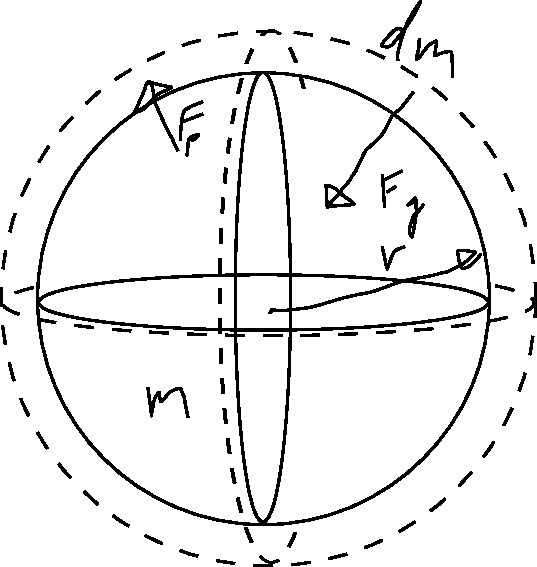
\includegraphics[width=0.32\textwidth]{figurer/hydrostatic_equillibrium.pdf}
    \caption{Kladd: The forces acting on a thin shell $\dd m$.}
    \label{fig: hydrostatic equillibrium}
\end{figure}

Both the Newtonian limit and the TOV equation are equations of \emph{hydrostatic equilibrium}, where the forces on a small volume of the fluid cancel out.
In the case of the TOV equation, we tacitly assumed hydrostatic equilibrium when we gave the fluid a rest frame where we could write $v_\mu = (v_0, 0, 0, 0)$ globally.
We can eliminate the equation for mass by differentiating \autoref{Newtonian limit TOV} with respect to $\tilde r$.
This gives us a single equation for hydrostatic equilibrium in the Newtonian limit,
%
\begin{equation}
    \label{Newtonian limit TOV single equation}
    \odv{}{\tilde r} 
    \left( \frac{\tilde r^2}{\tilde u} \odv{\tilde p}{\tilde r}\right) 
    = -  k'' \tilde r^2  \tilde u, \quad
    k'' = 3 \frac{k_2 k_1}{k_3} = 4 \pi G \frac{u_0^2 r^2_0}{p_0}.
\end{equation}
This is a second order differential equation, so we need an new boundary condition in addition to $p(0) = p_c$.
Close to the center, we can see from \autoref{Newtonian limit TOV} that for a finite energy density, we must have $p'(0) = 0$, our second boundary condition.

One important model for stars is the \emph{polytrope}, which has an equation of state of the form $u = K p^\gamma$ for some constant $K$.
As we will see, this fits well as the Newtonian limit of many equations of state and can be used to make predictions such as the Chandrasekhar limit, which sets the upper limit of the mass of white dwarf stars to $M \approx 1.5 \, M_\odot$~\autocite{chandrasekharHighlyCollapsedConfigurations1935,glendenningCompactStarsNuclear2012}.
To write \autoref{Newtonian limit TOV single equation} on the standard form, we assume $\gamma \neq 1$ and introduce
%
\begin{equation}
    \tilde u = a \theta^{n}, \quad 
    n = \frac{1}{\gamma - 1}, \quad 
    a = \frac{u(p_c)}{u_0}, 
    \quad a^{\frac{\gamma - 2}{2}}C \xi = r, \quad 
    C =\sqrt{ \frac{K}{k''} \frac{\gamma}{\gamma - 1}}.
\end{equation}
%
$n$ is called the \emph{polytropic index} of the star.
Inserting these new variables into the equation of hydrostatic equilibrium gives
%
\begin{equation}
    \label{Lane Emden equation}
    \frac{1}{\xi^2} \odv{}{\xi} \left(\xi^2 \odv{\theta}{\xi} \right) + \theta^n = 0.
\end{equation}
%
This is called the Lane-Emden equation and was first used to model stars as early as 1870~\autocite{laneTheoreticalTemperatureSun1870}.
The boundary conditions $p(0) = p_c$ and $p'(0) = 0$ now read $\theta(0) = 1$ and $\theta'(0) = 0$.
The stellar radius is defined by the first zero of the Lane-Emden function above $\xi = 0$, $\theta(\xi_1) = 0$, so that
%
\begin{equation}
    \label{Radius polytrope}
    \frac{R}{r_0}= C \xi_1  a^{\frac{\gamma-2}{2}}. 
\end{equation}
%
The total mass of the star can be integrated using \autoref{mass relation dimensionless} and \autoref{Lane Emden equation},
%
\begin{equation}
    \frac{M}{m_0} = 3 k_2 a^{\frac{3\gamma-4}{2}} C^3 \int^{\xi_1}_0 \dd \xi \, \xi^2 \theta^n = [-3 k_2 \xi_1^2 \theta'(\xi_1)] a^{\frac{3\gamma-4}{2}}.
\end{equation}
%
Thus, given a specific equation of state, and thus $\gamma$, the mass-radius relationship is given by
%
\begin{equation}
    \label{Polytrope mass radius relationship}
    R \propto M^\beta, \quad \beta = {\frac{\gamma - 2}{3 \gamma - 4}}.
\end{equation}
%
\autoref{fig: mass radius relation polytropes} illustrates this relationship, in arbitrary units, for a series of different values of $\gamma$, as well as the dependence of $\beta$ on $\gamma$.
For most values of $\gamma$, the stellar radius will increase as the mass increases.
The only range within which the radius decrease as the mass increase is $\gamma \in \left(\frac{4}{3}, 2 \right)$.
At $\gamma = \frac{4}{3}$ and $\gamma = 2$, respectively the mass and radius become independent of the central density.
If included in our figure, these polytropes would correspond to a horizontal and a vertical line.
\todo[inline]{what about $\gamma = 1$?}

\begin{figure}[h]
    \centering
    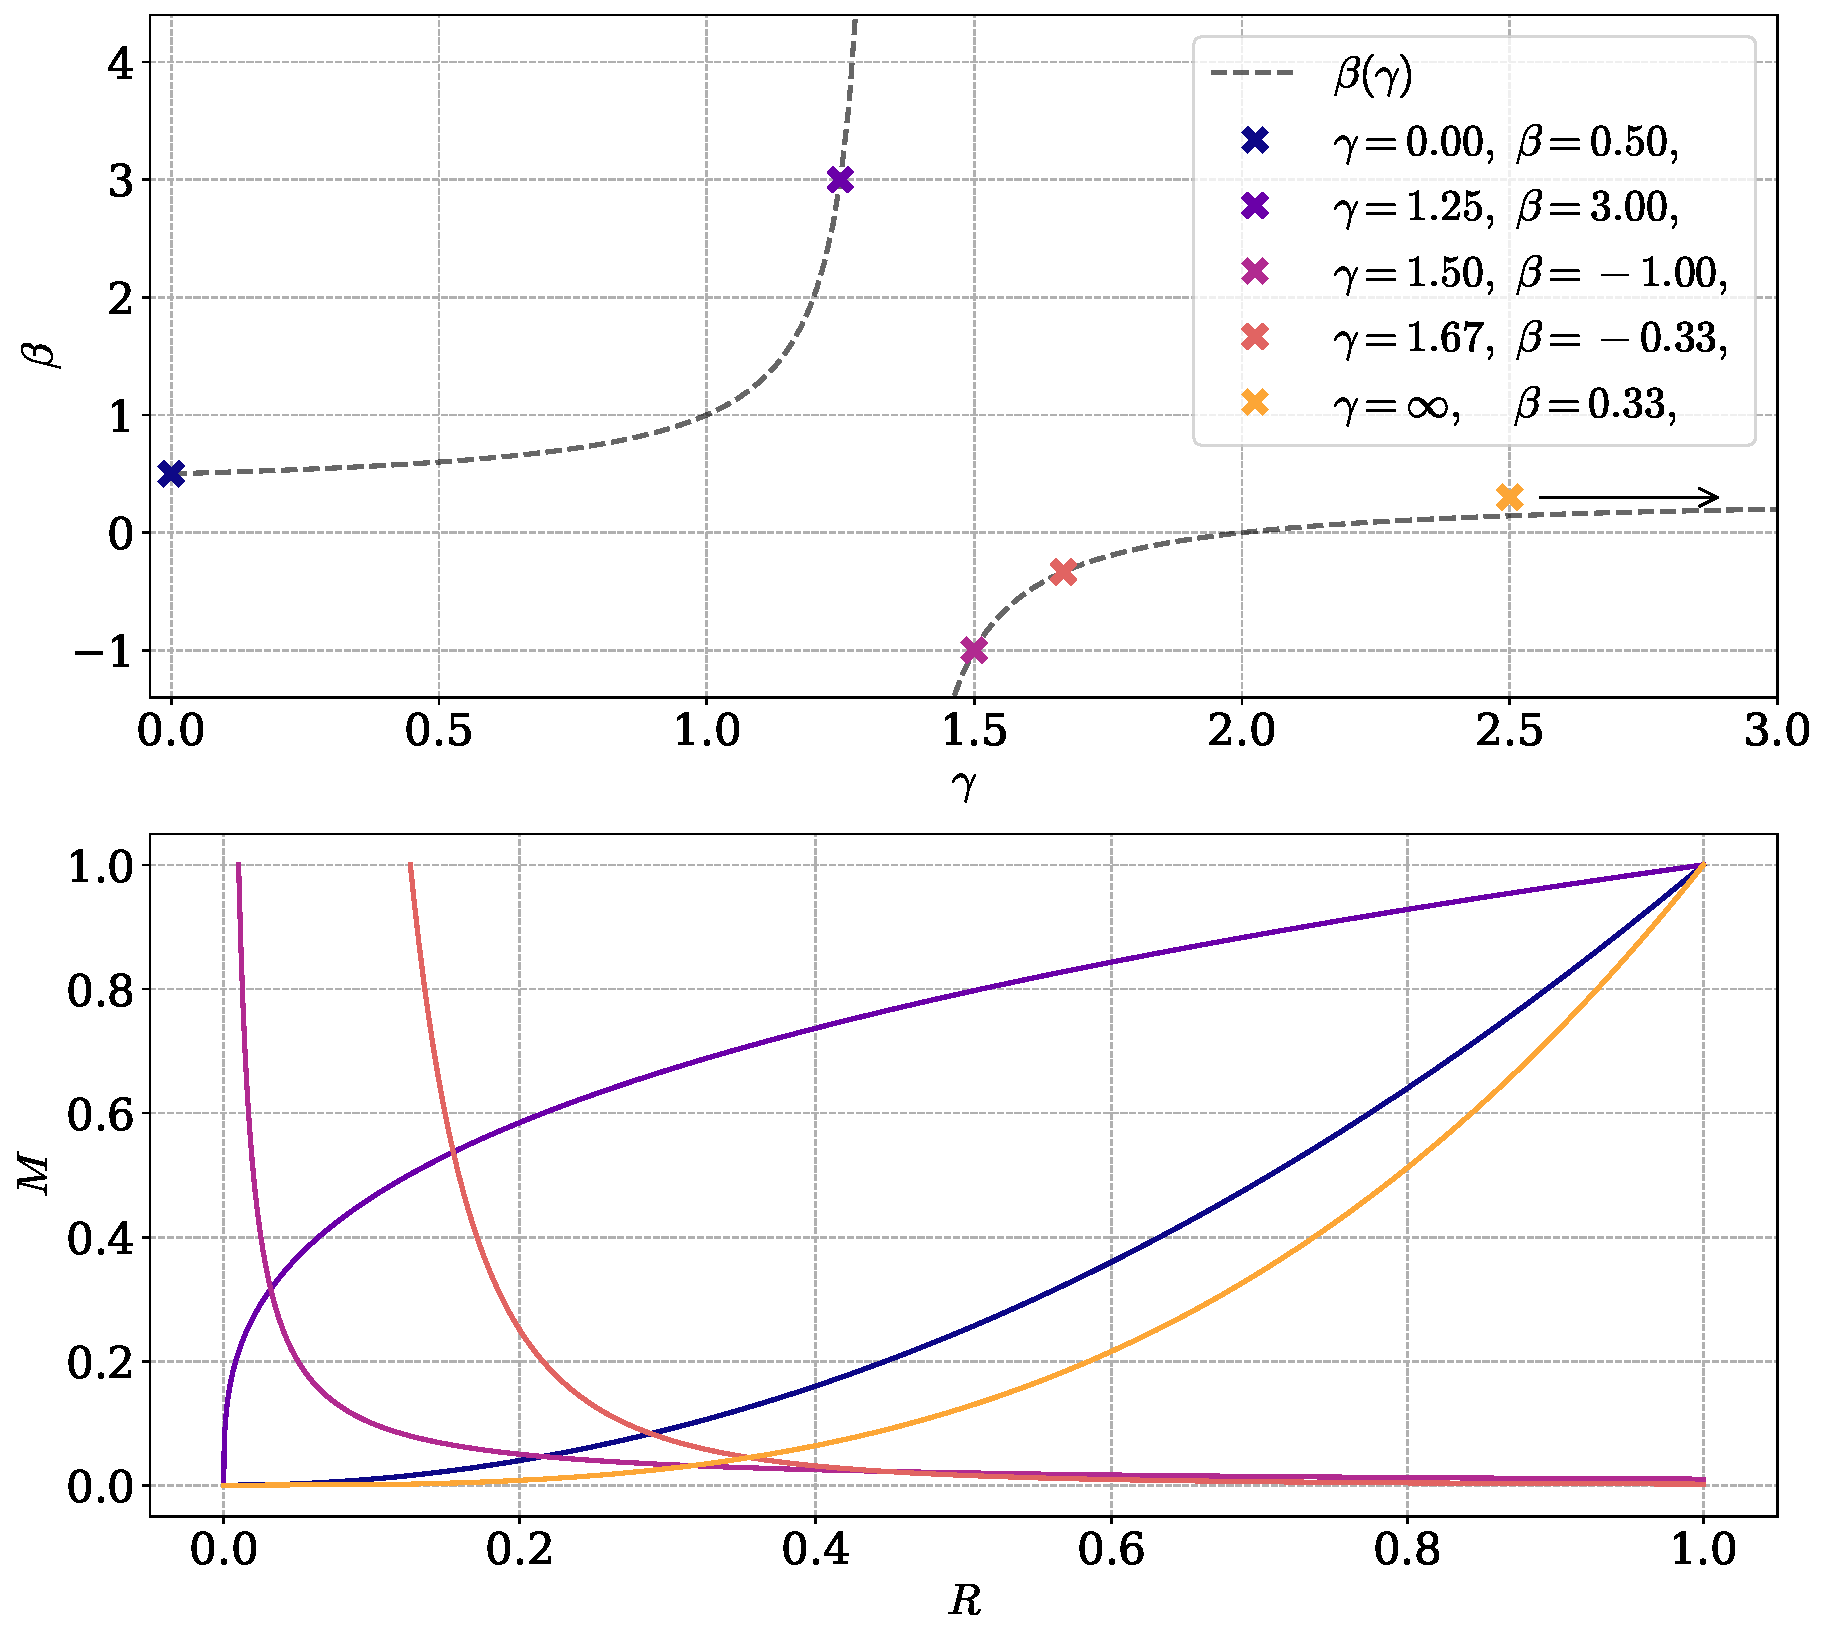
\includegraphics[width=\textwidth]{../scripts/figurer/mass_radius_relation_polytropes.pdf}
    \caption{
        Left: The dependence of $\beta$ on $\gamma$, together with a selection of points.
        Top: The mass-radius relation, in arbitrary units, for polytropes corresponding to the selected points on the left side. The color of the lines indicate which point it corresponds to.
        }
    \label{fig: mass radius relation polytropes} 
\end{figure}



\subsection{Incompressible fluid}
\label{subsection: incompressible fluid}

The simplest model for a star is one made up of an incompressible fluid, where the energy density is independent of the pressure.
This corresponds to a polytrope with $\gamma = \infty$.
In this case, the energy density of the star will be constant for a radius $r < R$, before it drops to zero,
%
\begin{equation}
    u(r) = u_0 \, \theta (R- r),
\end{equation}
%
where $u_0$ is a constant and $\theta(x)$ the Heaviside step function.
We choose $r_0 = R$.
Inserting this into the differential equation of the mass function, \autoref{mass relation dimensionless}, together with the boundary condition $m(0) = 0$, yields
%
\begin{equation}
    \tilde m(\tilde r) = k_2 \tilde r^3,
\end{equation}
%
when $r < R$.
For $r \geq R$, or $\tilde r \geq 1$, this relationship is simply constant $\tilde m(\tilde r) = \tilde m(1) = k_2$.
We choose $m_0$ to be the gravitational mass of the star, $M = \frac{4 \pi }{3} R^3 u_0$, which is equivalent to setting $k_2 = 1$.
Lastly, we choose $u_0 = p_0$, so that $k_3 = 1$.
With this the TOV equation, \autoref{TOV dimensionless}, becomes
%
\begin{equation} 
    \odv{\tilde p}{\tilde r} 
    = - k_1 \tilde r 
    \frac{(1 + \tilde p)(1 + 3 \tilde p)}{(1 - 2 k_1 \tilde r^2)}.
\end{equation}
%
This is a separable ODE, and each variable may be integrated separately.
Using
%
\begin{align}
    \int \frac{\dd x}{(1 + x)(1 + 3x)}
    = \frac{1}{2} \ln \frac{3x + 1}{x + 1} + \const , \quad
    \int \dd x \frac{x}{1 - 2 x^2} 
    = \frac{1}{4}\ln\left(1 - 2 x^2 \right)
    + \const,
\end{align}
%
together with the boundary condition $p(r = R) = 0$, we get 
%
\begin{equation}
    \label{pressure afo r incompressible}
    \tilde p(\tilde r) 
    = 
    - \frac{\sqrt{1 - 2 k_1} - \sqrt{1 - 2 k_1 \tilde r^2}}
    {3 \sqrt{1 - 2 k_1 } - \sqrt{1 - 2 k_1 \tilde r^2}}.
\end{equation}
%
We see that the star is entirely characterized by $k_1$.
In \autoref{fig: pressure incompressible fluid}, we have plotted the pressure as a function of radius for some values of $k_1$.
As $k_1$ approaches $0.\bar 4 = 4/9$, the pressure at the center of the star increases rapidly.
From the denominator of \autoref{pressure afo r incompressible} at $r\rightarrow 0$, we find the limit
%
\begin{equation}
    \label{mass radius constraint}
    k_1 = G \frac{M}{R} < \frac{4}{9}
\end{equation}
%
for the pressure to remain finite.
This is an absolute limit of the mass of an object given its radius or vice versa.
Although this limit is derived for a particular, unrealistic case, the more general statement can be shown to hold.
General relativity does not allow for a static solution with energy densities greater than this limit; any such configuration would collapse~\autocite{carrollSpacetimeGeometryIntroduction2019}.


\begin{figure}[h]
    \centering
    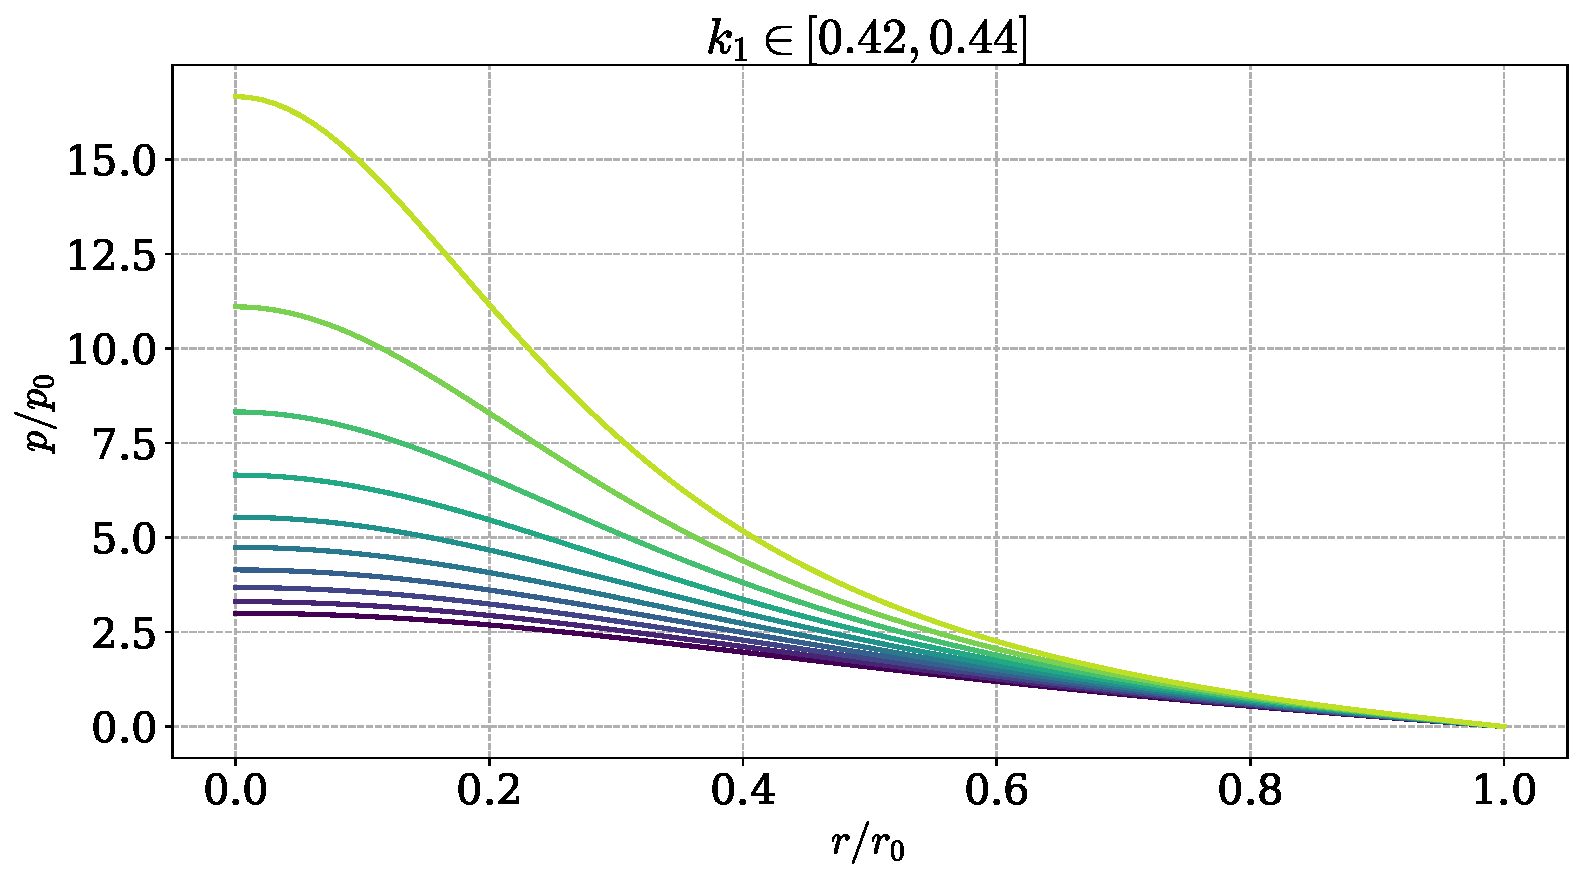
\includegraphics[width=0.8\textwidth]{../scripts/figurer/incompressible.pdf}
    \caption{The pressure in units of $p_0$, as a function of the radius, in units of $r_0$. The graphs with lighter color and higher pressure at $r = 0$ corresponds to higher values of $k_1$. The values of $k_1$ are linearly spaced.}
    \label{fig: pressure incompressible fluid}
\end{figure}

 
If we expand the solution \autoref{pressure afo r incompressible} in powers of $k_1$, then the leading order contribution is
%
\begin{equation}
    \tilde p(r) = \frac{1}{2} k_1 (1 - \tilde r^2).
\end{equation}
%
This is the Newtonian limit.
As a cross-check, we see that this solution obeys the equation of hydrostatic equillibrium in this limit, \autoref{Newtonian limit TOV}, as $\tilde u = 1$ and $k_2 = k_1 = 1$.
This is the general solution for an incompressible fluid in Newtonian gravity.
This solution does not have any upper limit for $k_1$; the limit $M/R < 4 / 9$ is purely relativistic phenomenon.
In \autoref{fig: pressure incompressible fluid newtonian}, the Newtonian approximation is compared to the full, relativistic solution.
We see that the Newtonian approximation is highly accurate for $k_1$ less than around $0.01$.


\begin{figure}[h]
    \centering
    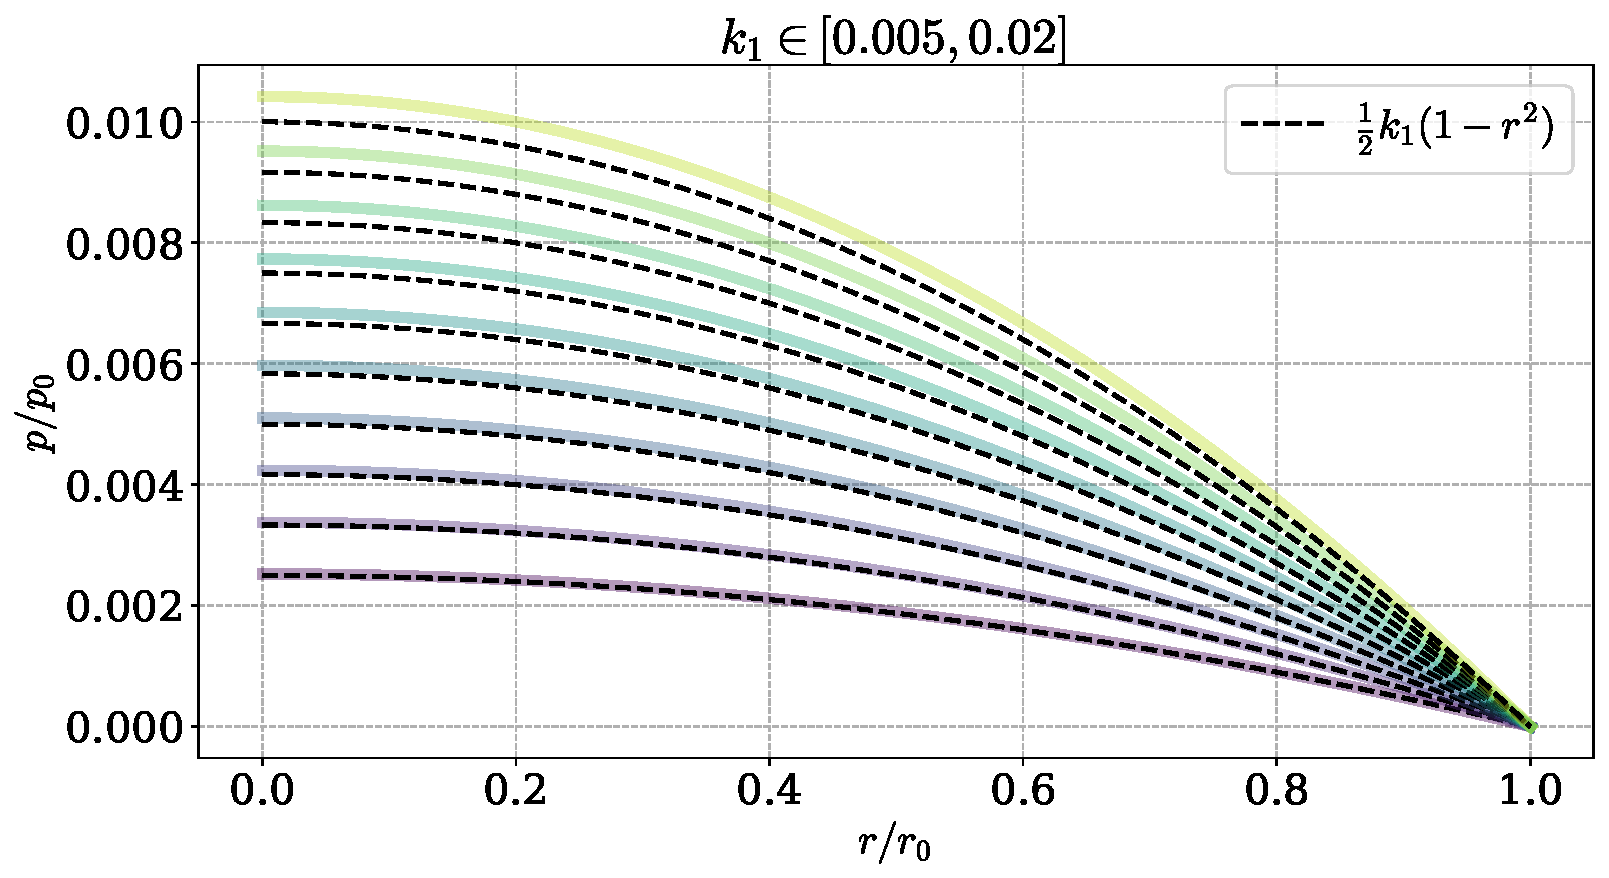
\includegraphics[width=0.8\textwidth]{../scripts/figurer/incompressible_newt.pdf}
    \caption{The pressure in units of $p_0$, as a function of the radius, in units of $r_0$. The wide, colored lines correspond to the full relativistic solution, while the dashed lines is the Newtonian approximation, for the same value of $k_1$. The values of $k_1$ are linearly spaced.  }
    \label{fig: pressure incompressible fluid newtonian}
\end{figure}


    \section{A star of cold, non-interacting fermions}
\label{section: cold fermi star}

This section is based on~\autocite{glendenningCompactStarsNuclear2012,andersenIntroductionStatisticalMechanics2012,kapustaFiniteTemperatureFieldTheory2006}.

In this section, we will study a simple model of a star made up of non-interacting, cold neutrons.
This is one of the earliest models used to study neutron stars, the remenants of massive stars~\autocite{glendenningCompactStarsNuclear2012}.
For this model, we use results derived in \autoref{section: fermions}.



\subsection{Thermodynamics and the equation of state}

The total energy $U$ is related to the grand canonical free energy $F$ by a Legendre transformation,
%
\begin{equation}
    F(T, V, \mu) = U - T S - \mu Q, \quad \dd F = - S \dd T - p \dd V - Q \dd \mu.
\end{equation}
%
Here $T = {1}/{\beta}$ is temperature, and $S$ entropy,  $p$ pressure, and $V$ volume.
$Q$ is some conserved charge, in our case the number of particles minus antiparticles, and $\mu$ is the corresponding chemical potential.
These thermodynamic variables are related to the free energy by
%
\begin{equation}
    S = - \pdv{F}{T} = \beta^2 \pdv{F}{\beta}, \quad
    Q = - \pdv{F}{\mu}, \quad
    p = - \pdv{F}{V}.
\end{equation}
%
When the free energy can be written as $F = V \Eff$, where the free energy density $\Eff$ is independent of the volume $V$, then $\Eff = - p$ and
%
\begin{equation}
    \dd (V \Eff) = V \dd \Eff - p \dd V,
\end{equation}
%
allowing us to write
%
\begin{equation}
    \Eff(T, \mu) = u - Ts - \mu n, \quad
    \dd \Eff = -s \dd T - n \dd \mu,
\end{equation}
% 
where $s$ and $n$ are entropy and charge density, defined by
%
\begin{equation}
    s = - \pdv{\Eff}{T} = \beta^2 \pdv{\Eff}{\beta}, \quad
    n = - \pdv{\Eff}{\mu}.
\end{equation}
%
With this, we can write the energy density as~\autocite{andersenIntroductionStatisticalMechanics2012}
%
\begin{equation}
    u = \pdv{}{\beta} \left(\beta \Eff\right) + \mu n.
\end{equation}
%

We calculate the free energy density of non-interacting fermions in \autoref{section: fermions}, with the result \autoref{free energy fermions},
%
\begin{equation}
    \Eff = - 
    \frac{2}{\beta}\int \frac{\dd^3 p}{(2 \pi)^3} 
    \left[
        \beta \omega
        +
        \ln\left(1 + e^{-\beta(\omega - \mu)}\right)
        + 
        \ln\left(1 + e^{-\beta(\omega + \mu)}\right)
    \right],
\end{equation}
%
where $\omega = \sqrt{p^2 + m^2}$.
The first term in the integral is the divergent vacuum energy, which must be renormalized.
We can drop this term; it does not have any observable effects on our results, as we are interested in relative pressure and energy density.
With this, we find the charge density
%
\begin{equation}
    n = \frac{1}{\pi^2} \int \frac{\dd^3 p}{(2 \pi)^3} [n_f(\omega - \mu) - n_f(\omega + \mu)],
\end{equation}
%
where
%
\begin{equation}
    n_f(\omega) = \frac{1}{e^{\beta \omega} + 1}.
\end{equation}
%
is the Fermi-Dirac distribution.
Using this, we find that the energy density is
%
\begin{equation}
    \label{energy density}
    u = \frac{1}{\pi^2} \int_0^\infty \dd p\, p^2 \, \omega \, [n_f(\omega - \mu) + n_f(\omega + \mu)].
\end{equation}
%
As expected, this is the energy per mode times the density of states, integrated over all modes.
To write the pressure, $p = - \Eff$ in terms of an integral over the Fermi-Dirac distribution, we integrate by parts.
We have
%
\begin{equation}
    \int_0^\infty \dd p \, p^2 \ln\left[1 + e^{-\beta(\omega \pm m)}\right]
    = 
    \frac{1}{3} p^3\ln\left[1 + e^{-\beta(\omega \pm m)}\right] \bigg |_0^\infty
    + 
    \frac{1}{3} \int_0^\infty \dd p \, \frac{ \beta p^4}{\omega}n_f(\omega \pm \mu),
\end{equation}
%
where the boundary term vanishes.
This allows us to write the pressure as 
%
\begin{equation}
    \label{pressure}
    p = \frac{1}{3} \int_0^\infty \dd p \, \frac{p^4}{\omega} [n_f(\omega - \mu) + n_f(\omega + \mu)]
\end{equation}



We are interested in the $T = 0$ limit.
In this case, the Fermi distribution becomes a step function, $n_f(\omega) = \theta(-\omega)$.
Without loss of generality, we assume that $\mu > 0$, i.e., we are dealing with an abundance of matter compared to anti-matter.
The dispersion relation $\omega = \sqrt{p^2 + m^2}$ is always positivive.
This means that the contribution to thermodynamic quantities from anti-particles vanish, as the integral is multiplied with $n_f(\omega + \mu) = \theta(-\omega - \mu)$, where the argument $-\omega - \mu$ is strictly negative on the domain of integration.
At zero temperature, the only dynamics are due to the degeneracy pressure of the fermions, that is, due to the Pauli exclusion principle.
There are no thermal fluctuations that can create a particle-antiparticle pair.
Thus, if the system has a positive chemical potential, it will contain no antiparticles.
Furthermore, if $\mu< m$, then integrand multiplied with $n_f(\omega - \mu)$ is also zero in the whole domain of integration.
It is only when $\mu\geq m$ that it is energetically favorable for the system to be in a state with particles.
We define the Fermi momentum $p_f$ by $\mu = \sqrt{\smash{p_f}^2 + m^2}$. 
In the zero-temperature limit, we can then rewrite any integral over the Fermi distribution as
%
%
\begin{equation}
    \int_0^\infty \dd p \, [f(p) n_f(\omega - \mu) + g(p) n_f(\omega - \mu)]= \int_0^{p_f} \dd p \, f(p).
\end{equation}
%
The charge density is thus
%
\begin{equation}
    n = \frac{1}{\pi^2} \int_0^{p_f} \dd p\, p^2 = \frac{p_f^3}{3 \pi^2}.
\end{equation}
%
At $T = 0$, this is the particle number density, as there are no antiparticles.
This density is given by the chemical potential and vanishes when $\mu \leq m$, i.e. when the free energy cost of creating a particle is positive.
We can write the energy density and pressure integrals, \autoref{energy density} and \autoref{pressure}, as
%
\begin{align}
    u &= \frac{1}{\pi^2} \int_0^{p_f} \dd p \,
    p^2 \sqrt{p^2 + m^2}
    = \frac{m^4}{\pi^2} \int_0^{x_f} \dd x \, x^2 \sqrt{x^2 + 1}, \\
    p & = \frac{1}{3 \pi^2} \int_0^{p_f} \dd p \,  \frac{p^4}{\sqrt{p^2 + m^2}} 
    = \frac{m^4}{3 \pi^2} \int_0^{x_f} \frac{\dd x \, x^4}{\sqrt{x^2 + 1}}.
\end{align}
% 
We have defined $x = p / m$ and $x_f = p_f/m$.
These integrals can be evaluated exactly as
%
\begin{align}
    \int_0^a \dd x \, x^2 \sqrt{x^2 + 1} 
    & = \frac{1}{8} 
    \left[\sqrt{a^4 + 1}(2 a^3 + a) - \arcsinh\left(a\right)\right], \\
    \int_0^a \dd x \, \frac{x^4}{\sqrt{x^2 + 1} }
    & = \frac{1}{8} 
    \left[\sqrt{a^2 + 1}(2 a^3 - 3a) + 3\arcsinh\left(a\right)\right].
\end{align}
%
We introduce the characteristic energy and number density,
% 
\begin{equation}
    u_0 = \frac{m^4}{8 \pi^2}, \quad n_0 = \frac{u_0}{m},
\end{equation}
%
which allows us to write the thermodynamic variables as
%
\begin{align}
    \label{Fermi gas particle density}
    n &= \frac{8}{3}  n_0 \,x_f^3 \\
    \label{Fermi gas energy density}
    u &= u_0
    \left[(2x_f^3 + x_f) \sqrt{1 + x_f^2} - \arcsinh\left(x_f\right)\right], \\
    \label{Fermi gas pressure}
    p &= \frac{u_0}{3}
    \left[(2x_f^3 - 3x_f) \sqrt{1 + x_f^2} + 3\arcsinh\left(x_f\right)\right].
\end{align}
%
We have thus chosen $u_0 = p_0$, or equivalently set $k_3 = 1$.
This is natural in the case of a relativistic fluid.




\subsection{Limits}

In the non-relativistic limit, as the chemical potential approaches $m$ and thus $p_f \ll m$, the lowest order contributions to the energy density and pressure are given by the Taylor series around $x_f = 0$,
%
\begin{align}
    \tilde u(x_f) &= \frac{8}{3}x_f^3 + \frac{4}{5} x_f^5 + \Oh(x_f^7),  \\
    \tilde p(x_f) &= \frac{8}{15}x_f^5 + \Oh(x_f^7).
\end{align}
%
By neglecting terms of order $x_f^7$ and higher, we can write this as
%
\begin{equation}
    \tilde u = \tilde n + \frac{4}{5} \left( \frac{8}{3} \tilde n \right)^{5/3},
    \quad
    \tilde p =  \frac{8}{15} \left( \frac{8}{3} \tilde n \right)^{5/3}.
\end{equation}
%
The leading order contribution to the energy density is the rest mass of the particles.
This term does not contribute to the pressure.
As discussed earlier, the non-relativistic limit corresponds to $k_3 \ll 1$, if we chose units so that $\tilde u \approx \tilde p$, or $\tilde u \gg \tilde p$ if we demand that $k_3 = 1$.
We see that $x_f \rightarrow 0$ corresponds to the latter case.
By including only the leading order term, we can eliminate the Fermi momentum and write the equation of state in the non-relativistic limit as $u_{\mathrm{nr}} = k p^\frac{3}{5}$ where $k = 8/3 \cdot (15/8)^{3/5}$.
The non-relativistic approximation of the cold fermions is thus a polytrope with $\gamma = \frac{5}{3}$.
As we see from \autoref{fig: mass radius relation polytropes}, this is within the range where the mass decreases with the size of the star.

In the ultrarelativistic limit, where $p_f \gg m$, the leading order contributions to the pressure and energy density are
%
\begin{equation}
    \tilde u = 2 x_f^4, \quad \tilde p = \frac{2}{3} x_f^4, 
\end{equation}
%
and we get the particularly simple equation of state for the ultrarelativistic limit, $ u_{\mathrm{ur}} = 3 p $, which we recognize as the formula for radiation pressure.
The equation of state $\tilde u(\tilde p)$ in two different regimes are shown in \autoref{fig: equation of state fermi fluid}.
The full equation of state is compared to the non-relativistic and ultrarelativistic approximations.

\begin{figure}[h]
    \centering
    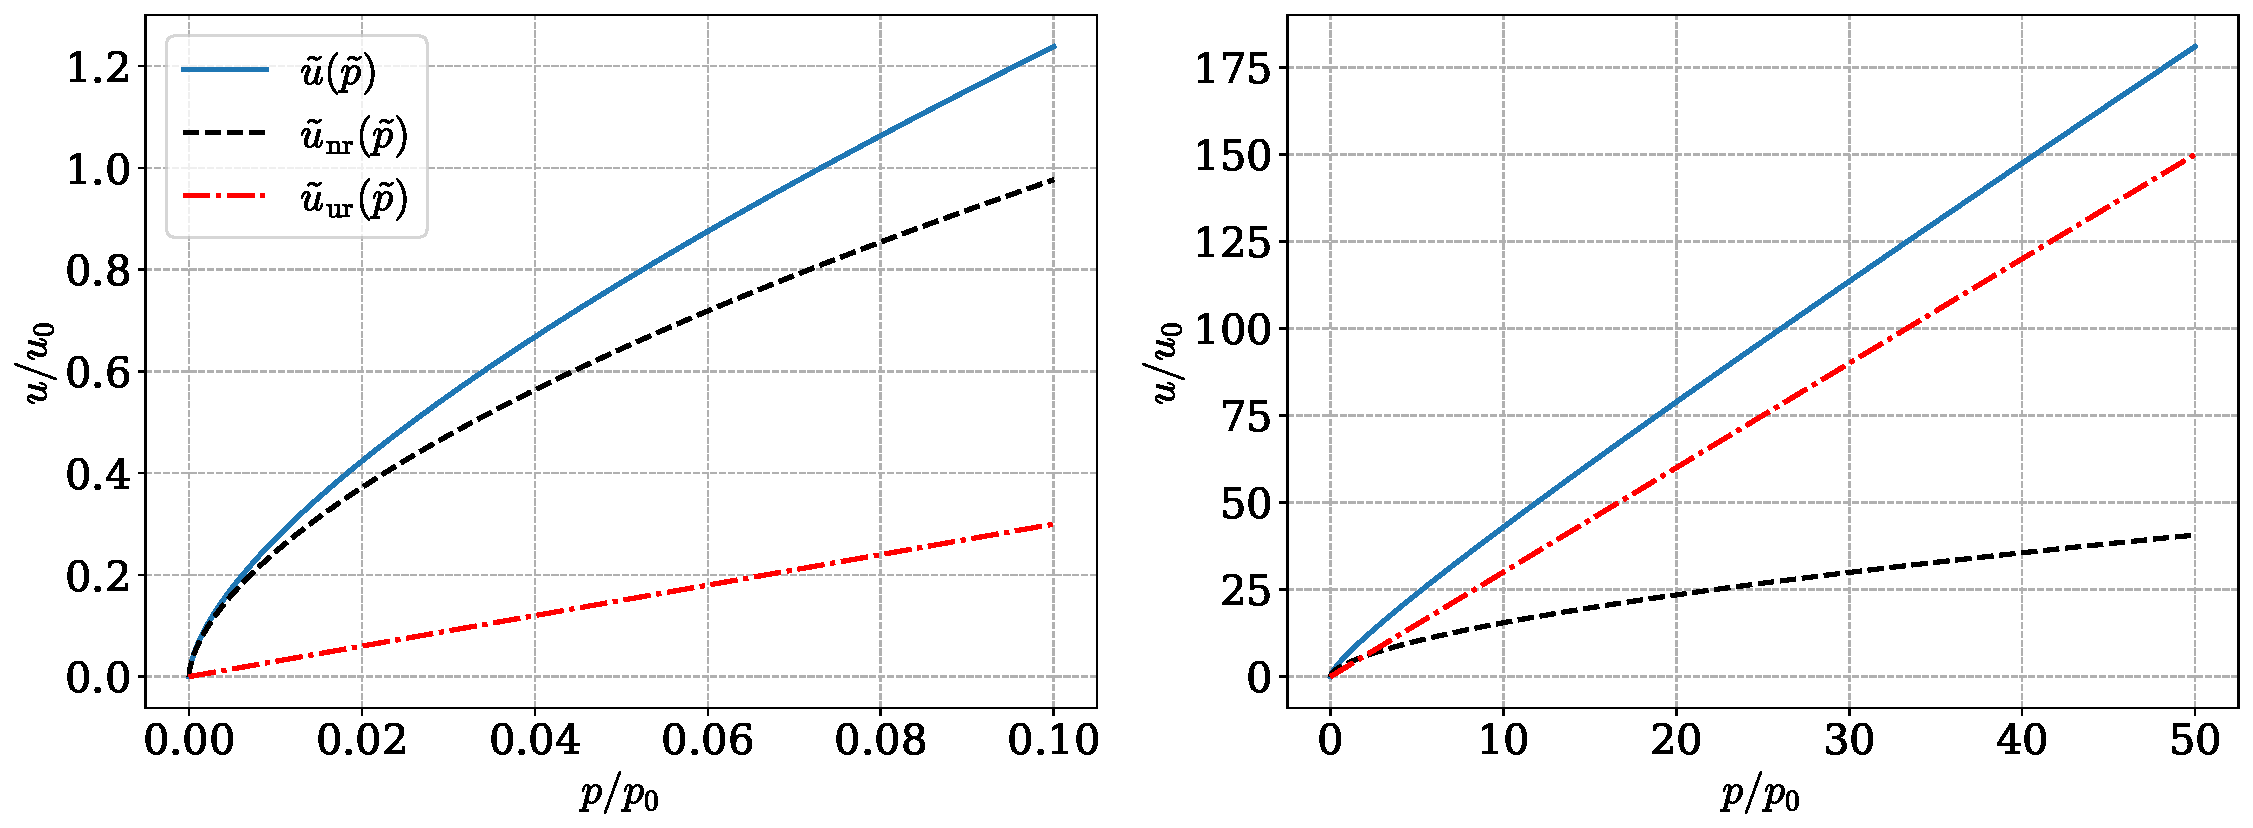
\includegraphics[width=\textwidth]{../scripts/figurer/fermi_eos.pdf}
    \caption{The equation of state of a cold Fermi gas. Both pressure and energy density is normalized to their characteristic quantities, $p_0$ and $u_0$. The equation of state is compared to the non-relativistic approximation, $\tilde u_{\mathrm{nr}}$ as well as the ultrarelativistic approximation, $\tilde u_{\mathrm{ur}}$, in two different regimes.}
    \label{fig: equation of state fermi fluid}
\end{figure}




\subsection{Units}

The equation of state has given us the characteristic energy density and pressure, $u_0$ and $p_0$. 
If we demand
%
\begin{equation}
    G \frac{m_0}{r_0} = \frac{4 \pi }{3}\frac{r_0^3 u_0}{m_0} = 1,
\end{equation}
%
we have two equations and two unknowns, $m_0$ and $r_0$.
This thus defines a complete set of units.
We are using the cold Fermi-gas as a model for a neutron star, an the mass of the fermion $m$ is therefore the neutron mass, \autoref{mass of neutron}, $m_N = 1.674 \cdot 10^{-27} \, \text{kg}$.
After reinstating $\hbar$ and $c$ in metric units, we get
%
\begin{align}
    u_0 &= p_0 = \frac{m^4}{8 \pi^2}\frac{c^5}{\hbar^3} 
    = 2.056\cdot10^{35}  \, \text{J}\,\text{m}^{-3}, \\
    m_0 &= \frac{c^4}{\sqrt{\frac{4 \pi}{3} u_0 G^3} }
    = 1.598 \cdot 10^{31} \, \text{kg}
    = 8.032 \, M_\odot, \\
    r_0 &= \frac{G m_0}{c^2} = 11.86 \, \text{km}. % sjekk
\end{align}
%
From this, we expect our star to have a mass of the order of a solar mass $M_\odot$ and a radius of the order of kilometers, without solving the TOV equation.




\subsection{Numerical results}



With the energy density, \autoref{Fermi gas energy density}, and pressure, \autoref{Fermi gas pressure}, we can numerically solve the TOV equation given a central pressure $p_c$. 
This is done using an adaptive Runge-Kutta method, with the stop criterion $p(r) = 0$.
Description of the code and where to find it is given in \autoref{appendix: code}.
The top graph in \autoref{fig: pressure and mass as a function of radius} shows the pressure, normalized to the central pressure $p_c$, as a function of radius, normalized to the corresponding stellar radius $R$.
The boundary conditions are logarithmically spaced.
The lower graph in \autoref{fig: pressure and mass as a function of radius} shows the mass, normalized to the total mass $M = m(R)$, as a function of the radius, again normalized to the stellar radius.
As in the case of an incompressible fluid, the pressure follows a half bell-shaped curve, with a peak that becomes narrower as the central pressure increases.
The black dashed line corresponds to the solution with the maximum mass, which will discuss shortly.
We see that the pressure and mass curves change most drastically when the central pressure is higher than that corresponding to the most massive star.

\begin{figure}[H]
    \centering
    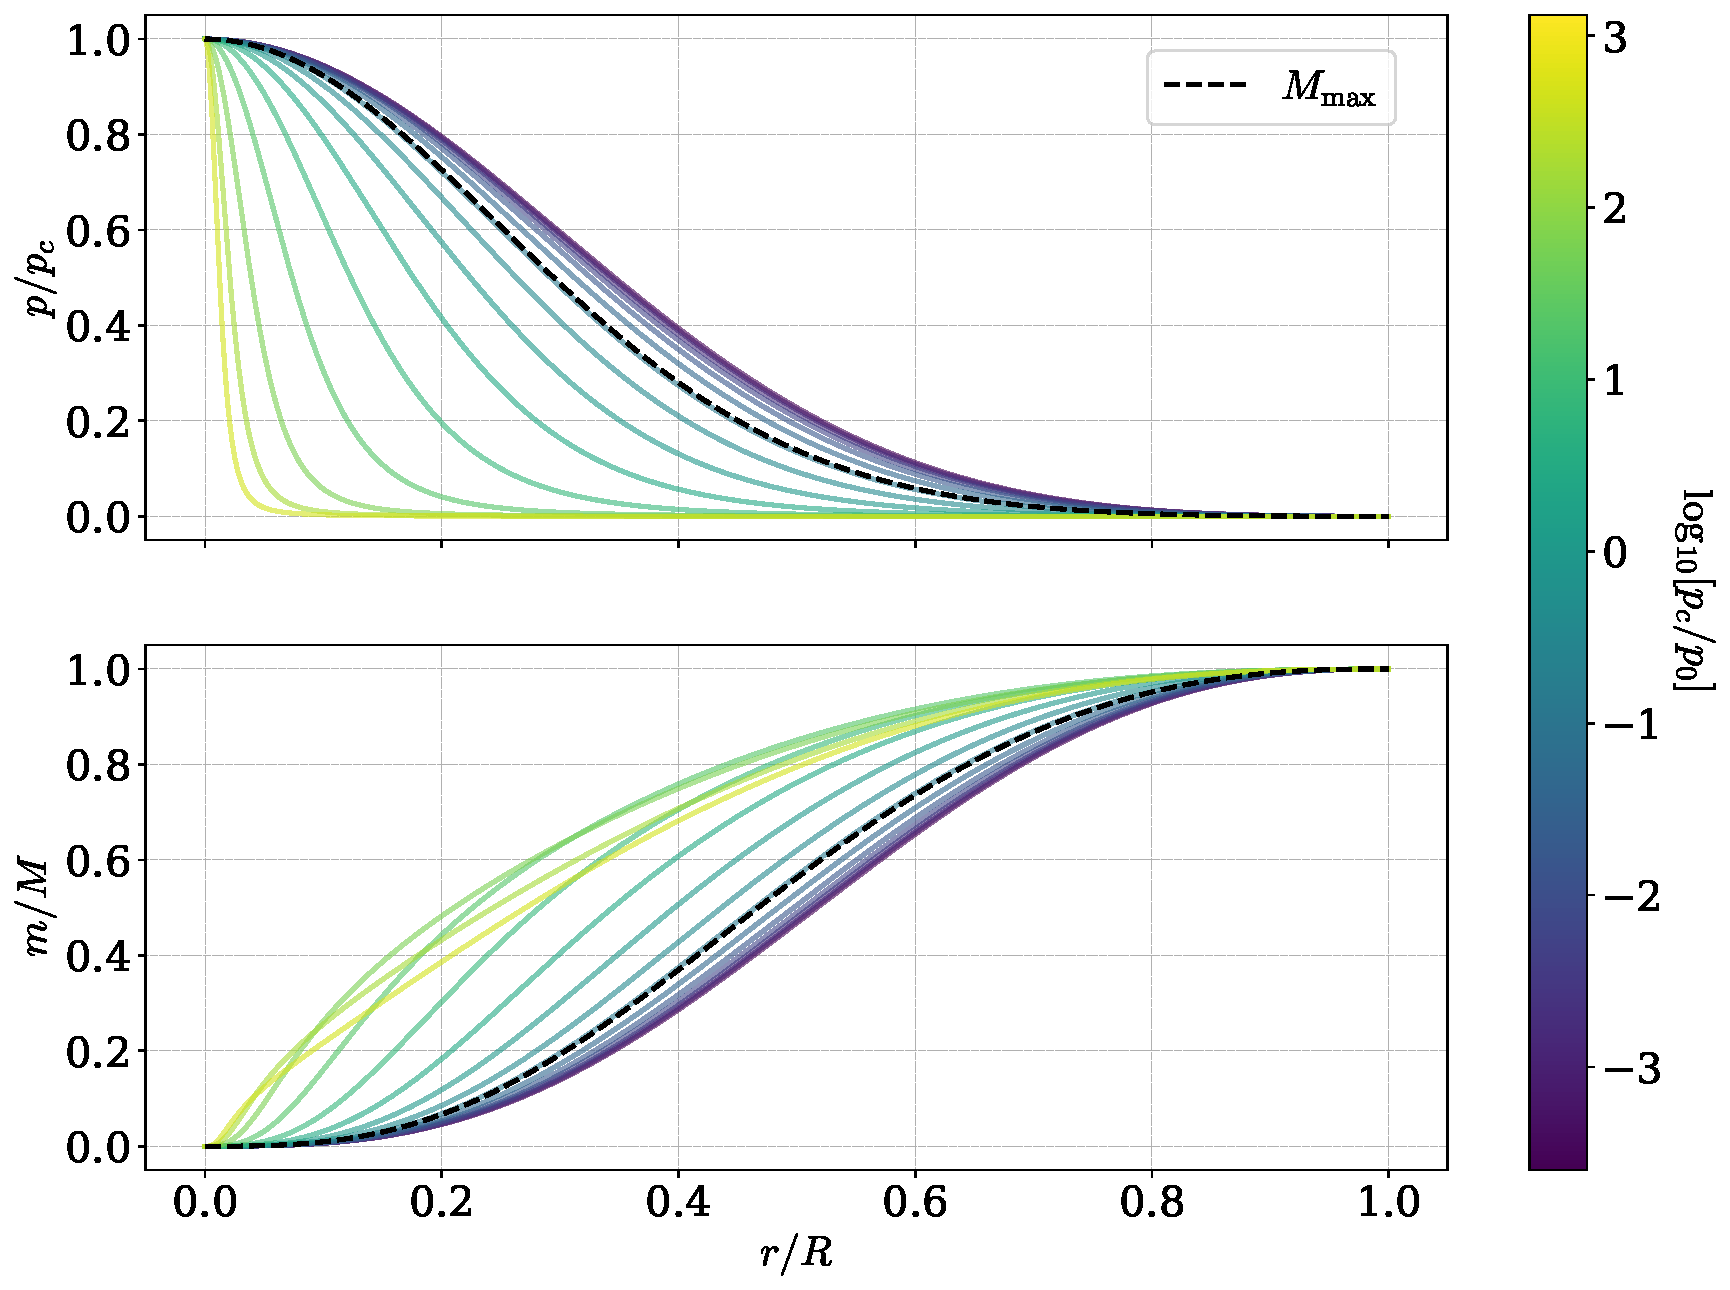
\includegraphics[width=0.9\textwidth]{../scripts/figurer/pressure_mass.pdf}
    \caption{
        Top: The pressure normalized to central value, as a function of radius, normalized to the stellar radius.
        Bottom: The mass normalized to the total mass, as a function of radius, normalized to the stellar radius. 
        This is plotted for several different values of central pressure, which is indicated by the color scheme.
        }
    \label{fig: pressure and mass as a function of radius}
\end{figure}

In \autoref{fig: mass radius relationship fermi gas}, we see the relationship between the mass and radius of the star.
This line is parametrized by the base-10 logarithm of the central pressure, $p(0)$, normalized by $p_0 = u_0$.
The cross marks the maximum mass, $M_\mathrm{max} = 0.711 \, M_\odot$, which corresponds to a radius of $R = 9.20 \, \mathrm{km}$.
This matches the results obtained by Oppenheimer and Volkoff~\cite{oppenheimerMassiveNeutronCores1939}, $M_\mathrm{max} = 0.71$.
In their 1939 paper, Oppenheimer and Volkoff computed five data points in the mass-radius plane.
The results are marked by blue circles in \autoref{fig: mass radius relationship fermi gas}.
We find good agreement between the three points closest to the maximum value and our results.
However, the two results of Oppenheimer and Volkoff furthest away differ significantly from our results.
The black dashed line is the absolute mass-radius constraint, \autoref{mass radius constraint}, and any stable configuration must be on the right side of this line.
As we predicted from looking at the non-relativistic equation of state, the mass decreases with the star's radius, at least for stars with low central pressure.


In \autoref{fig: mass radius relationship comparison}, we compare the mass-radius relationship obtained from the full theory with results from approximations.
The lowest line is obtained by using both the full TOV equation and the exact equation of state.
The next line above is obtained using the non-relativistic equation of state together with the full TOV equation.
The second uppermost line is obtained from the exact equation of state and the Newtonian approximation for the TOV equation.
The uppermost line uses both the Newtonian approximation to the TOV equation and the non-relativistic approximation for the equation of state.
This last line corresponds to a polytrope in Newtonian gravity, as we studied in \autoref{subsection: Newtonian limit and polytropes}.
Unlike the other systems, it does not seem to have an upper limit for the mass, as expected.


\begin{figure}[H]
    \centering
    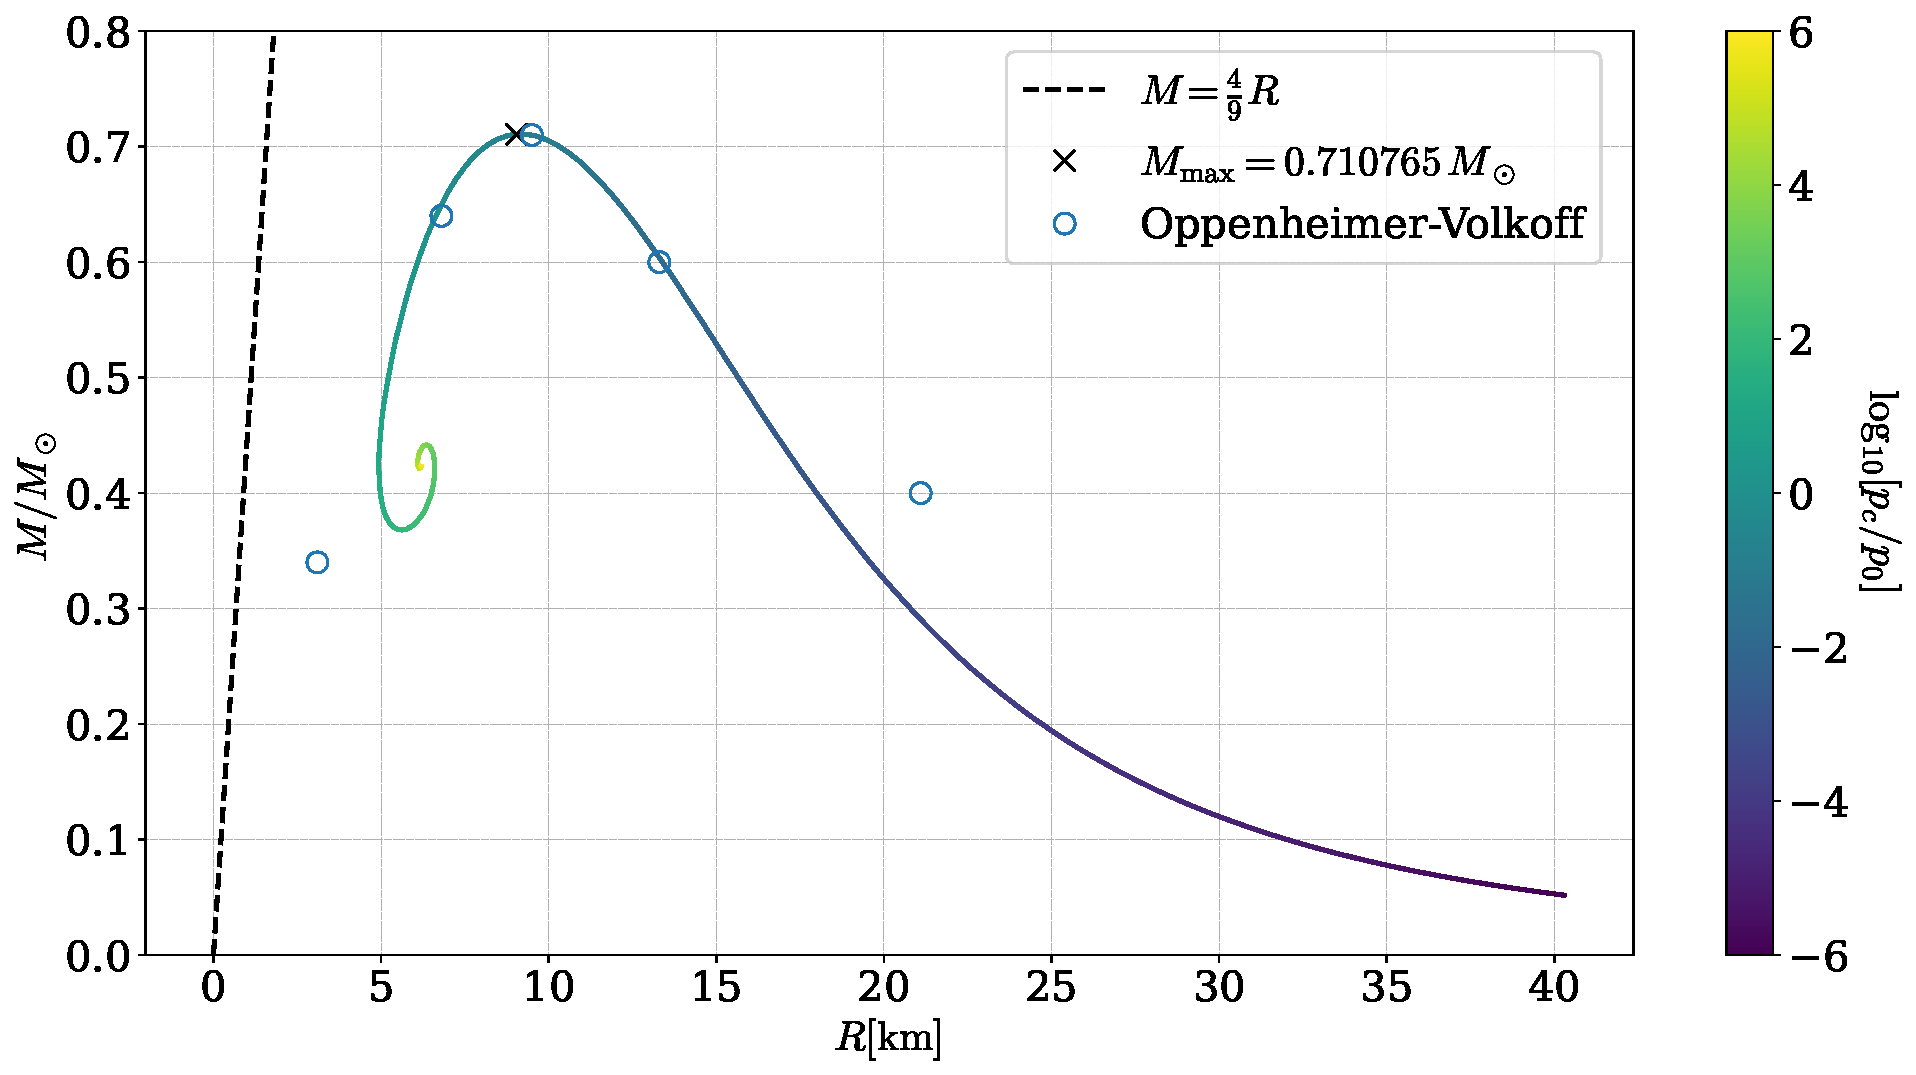
\includegraphics[width=\textwidth]{../scripts/figurer/mass_radius_neutron.pdf}
    \caption{The mass-radius relationship of a star made of a cold gas of neutrons. The line is parametrized by the central pressure $p_c$. The corss indicate the maximum mass solution. The blue circles are results form the 1939 paper of Oppenheimer and Volkoff~\autocite{oppenheimerMassiveNeutronCores1939}.}
    \label{fig: mass radius relationship fermi gas}
\end{figure}

\begin{figure}[H]
    \centering
    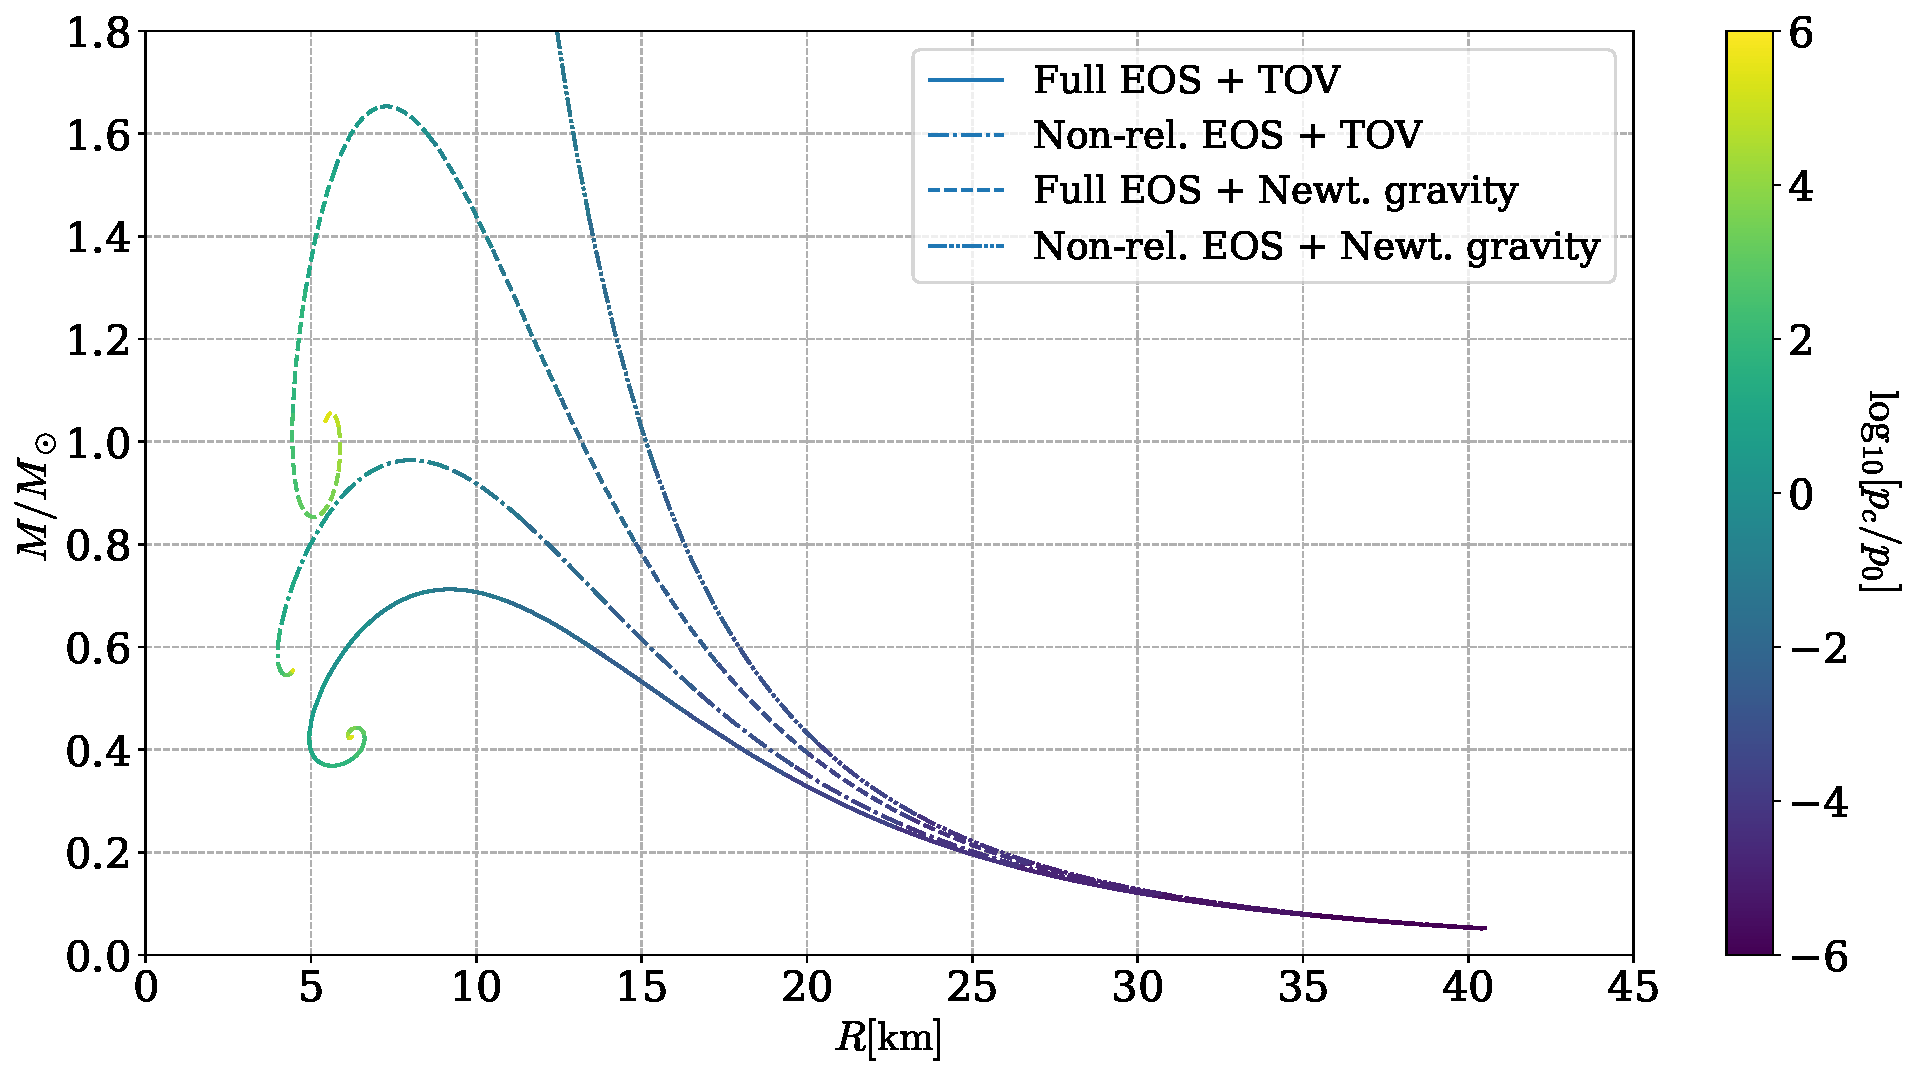
\includegraphics[width=\textwidth]{../scripts/figurer/mass_radius_comparison.pdf}
    \caption{The mass-radius relationship of a cold gas of neutrons. The lowest line is obtained from the TOV equation and full equation of state. The middle line is from the TOV equation and the non-relativistic equation of state. The upper line is obtained from the Newtonian approximation of the TOV equation and the non-relativistic equation of state.}
    \label{fig: mass radius relationship comparison}
\end{figure}




\subsection{Upper bound and stability}
\todo[inline]{Utvid om stability}

For any equation of state, the TOV equation will give a one-parameter\todo{Can there be multiple branches?} family of stars, parametrized by the central pressure $p_c$.
This leads to the possibility of an \emph{absolute maximum} mass for a given equation of state.
In the case of a non-interacting neutron, we found the limit to be $0.71 \, M_\odot$, in agreement with Oppenheimer and Volkoff.
To obtain a more general upper limit for the mass of neutron stars, or compact stars in general, one has to account for more general equations of state.
To constrain the equation of state, we assume firstly that $\odv{p}/{u} \geq 0$.
To justify this, take the non-relativisitc case, $u = n$, in which case the assumption is equivalent to $\odv{p}/{n} \geq 0$.
This says that an increase in particle density, for example, due to compression, will result in a rise in pressure.
This is an instance of Le Chatelier's principle; nature will counteract any change forced upon it.
The speed of sound in the fluid, $v_s$, is given by~\autocite{weinbergGravitationCosmologyPrinciples1972}\todo{Vis dette?}
%
\begin{equation}
    v_s^2 = \odv{p}{u}.
\end{equation}
%
A realistic fluid should not have a speed of sound greater than the speed of light, leading to the constraint $\odv{p}/{u} < 1$.
Using these general assumptions, Rhoades and Ruffini found an upper limit for neutron stars of $3.2 \, M_\odot$~\cite{rhoadesMaximumMassNeutron1974}.

An equation of state with a \emph{high} speed of sound, i.e., with a flat curve in the $p-u$-plane, is called \emph{stiff}.
From \autoref{fig: equation of state fermi fluid}, we see that the Newtonian equation of state is stiffer in the high-energy regime.
The most extreme case is the incompressible model we saw earlier, which breaks causality.
In general, a stiffer equation of state leads to a larger maximum mass.
This is intuitive; the TOV equation describes the balancing of forces from pressure and gravity, and if the pressure raises fast as the density increases, then it can sustain a large total mass before it collapses~\autocite{glendenningCompactStarsNuclear2012}.


Solutions to the TOV equation are systems in hydrostatic equilibrium.
However, as a pen perfectly balances on its edge, this does not imply stability.
When perturbed, a stable system returns back towards its equilibrium position as a marble in the bottom of a bowl.
On the other hand, an unstable system will amplify perturbations, leading to a collapse or an explosion.
We can make an intuitive argument for which configurations for a given family of stars are stable.
We will again assume that the equation of state, on a microscopic level, obeys Le Chatelier's principle in the form $\odv{p}/{n} > 0$.\todo{Er det en god antagelse?}
We can see that this holds for all the cases we are considering.
A star in equilibrium will find itself on the line parametrized by its central pressure, such as \autoref{fig: mass radius relationship fermi gas}.
In this case, a perturbation reducing the radius of the star will increase the central pressure as the particle density increases. \todo{Kan vi være helt sikre på dette?}
This is illustrated in \autoref{fig: fermi stability}.
A star in equilibrium at point A can be compressed to an out-of-equilibrium configuration, point B.
This point has a central pressure corresponding to the equilibrium state at point C.
As the equilibrium configuration at point C has a \emph{lower} mass than the configuration at B, it has a weaker gravitational effect.
Therefore, we would expect it to shrink further, as the central pressure of B is not enough to support its gravitational mass.
This compression will lead to an even higher central pressure.
We thus have a positive feedback loop, and the initial perturbation will continue to grow.
We can make a similar argument in the case where the mass increases with an increase in the central pressure.
Here, a compression will lead to a state in which central pressure corresponds to an equilibrium state with a \emph{higher} mass.
This state will thus tend to expand after a compression, counteracting the perturbation.
This gives us the following criterion for stability,
%
\begin{equation}
    \odv{M}{p_c} > 0.
\end{equation}

\begin{figure}[!h]
    \centering
    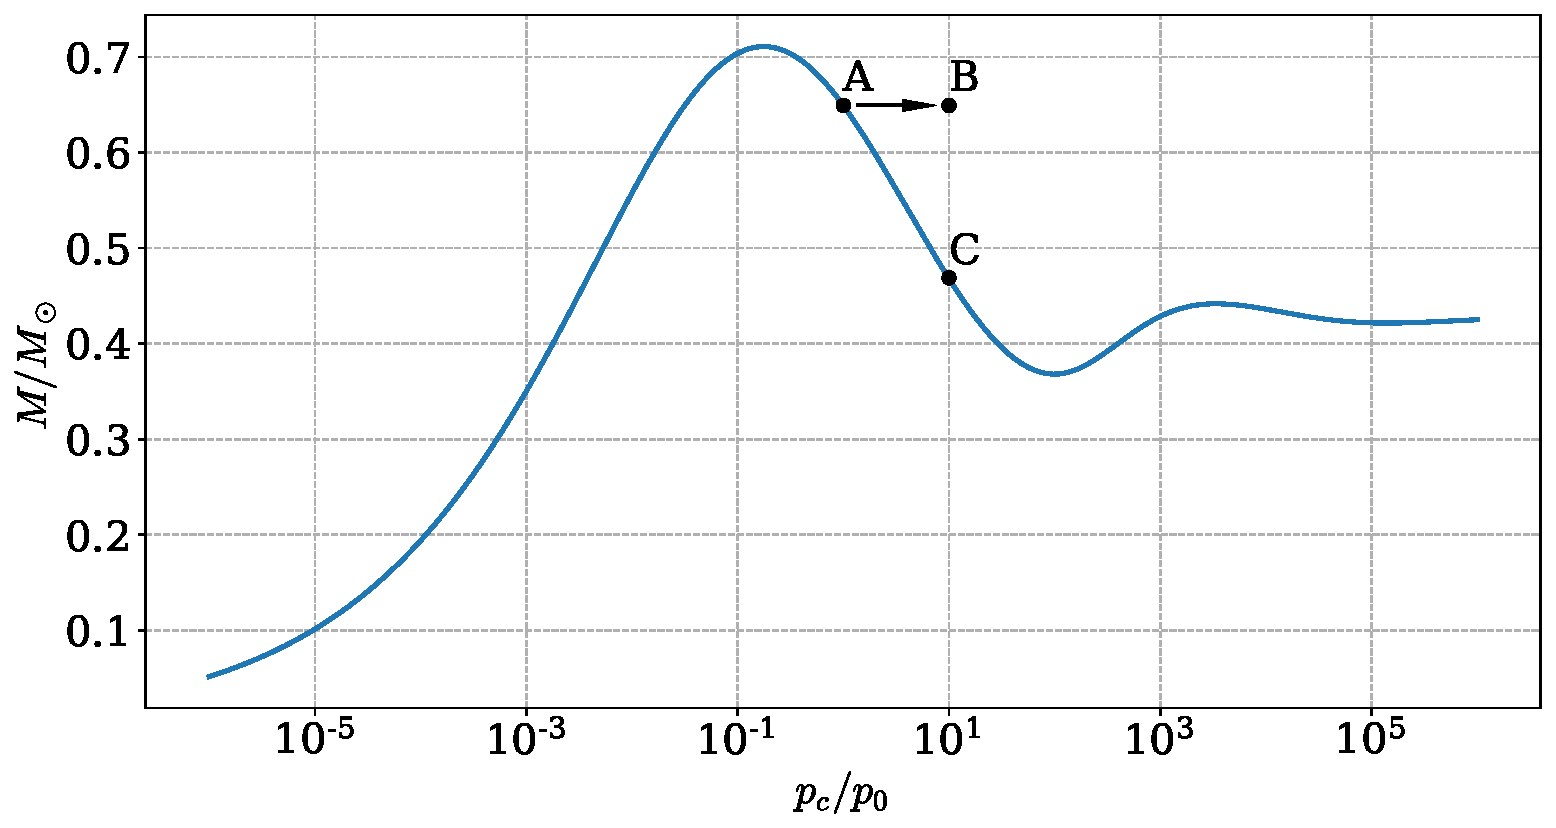
\includegraphics[width=0.7\textwidth]{../scripts/figurer/fermi_stability.pdf}
    \caption{
        The plot shows the mass, in units of solar masses, of a star of a cold gas of neutrons, as a function of the central pressure, normalized to the characteristic pressure.
    Point A denotes a position of equilibrium, which can be compressed to an out-of-equilibrium point, B, which has a central pressure corresponding to an equilibrium configuration, point C.
    }
    \label{fig: fermi stability}
\end{figure}

As it turns out, this is only a necessary requirement for stability.
To conduct a more rigorous study of stability, one must derive the equation of hydrostatic equilibrium with the addition of perturbations as time-dependent, radial oscillations.
This is done by discplacing a fluid elemet at a radius $r$ and time $t$ by $\delta r(r, t) = \sum_n A_n \xi_n(r) e^{i \omega_n t}$.
Here, $\xi_n$ are normal modes with frequencies $\omega_n$, $n \in \{0, 1, ...\}$.
The equation for the eigenmodes was first obtained by Chandrasekhar~\autocite{chandrasekharDynamicalInstabilityGaseous1964}, and can be written in the form of a Sturm-Liouville theory equation,
%
\begin{equation}
    \left[     \odv{}{r} \left( \Pi \odv{}{r}  \right) + Q + \omega_n W \right] \xi_n
    = 0,
\end{equation}
%
where $\Pi$, $Q$, and $W$ are functions of the pressure, energy density, particle density, $\alpha$, and $\beta$.
These quantities are thus given by a solution to the equilibrium problem~\cite{glendenningCompactStarsNuclear2012}.
This analysis is outside the scope of this thesis, but we summarize some important conclusions.
Stability is encoded in the sign of the square of the frequencies.
For $\omega_n^2>0$, the mode will remain oscillatory, while if $\omega_n^2<0$, it will grow exponentially.
Thus, if the system has \emph{any} modes such that $\omega_n^2<0$, it is unstable.
One mode $\omega_n$ will change stability at a critical point on the $M-R$ curve, where
%
\begin{equation}
    \odv{M}{u_c} = 0,
\end{equation}
%
and this will \emph{only} happen at critical points~\autocite{thorneGeneralRelativisticTheoryStellar1968}. Here, $u_c$ is the central energy density corresponding to $p_c$.
This is equivaent to the criterion $\odv{M}/{p_c} = 0$ as long as $\odv{p}/{u}$ is finite.
Whether or not the change is from a stable mode to an unstable one is dependent on whether or not the curve turns clockwise (a mode becomes stable) counterclockwise (a node becomes unstable)~\autocite{thorneGeneralRelativisticTheoryStellar1968}.
We know that very low-pressure, cold fermions are stable, which means that configuration with a radius larger than the maximum mas $0.71 \, M_\odot$ will be stable.
As illustrated in \autoref{fig: mass radius relationship fermi gas}, the curve then turns counterclockwise, and a new mode is made unstable each half turn.


    \chapter{Pion stars}
    \label{chapter: pion stars}
    As we found in \autoref{section: TOV equation}, the Tolman-Oppenheimer-Volkoff equation, \autoref{TOV}, determines the pressure as a function of the radius of a star given the equation of state and the central pressure.
From \autoref{chapter: thermodynamics}, we have various equations of state for the pion condensate.
In this chapter, we will apply these results to study pion stars, bosonic stars composed of a gravitationally bound pion condensate, first proposed by \citeauthor{brandtNewClassCompact2018}~\autocite{brandtNewClassCompact2018}.



\section{Units and limiting radius}

We can gain some insights by reviewing the characteristic quantities of the problem.
The characteristic mass and length, as discussed in \autoref{section: TOV equation}, are found by setting $k_1 = k_2 = k_3 = 1$.
These are the dimensionless constants of the TOV equation, \autoref{dimensionless constants TOV}.
At leading order, the bare constants $f$ and $\bar m$ are related to physical constants by $f = f_\pi$ and $m = m_\pi$, the pion decay constant and the pion mass.
Using the values for $f_\pi$ and $m_\pi$ as given in \autoref{section: units} and reinstating $c$ and $\hbar$, these quantities are given by
%
\begin{align}
    u_0 & =m_\pi^2 f_\pi^2 \frac{c}{\hbar^3}
    = 3.216\cdot 10^{33} \, \text{J}\,\text{m}^{-3}, \\
    m_0 & = \frac{c^4}{\sqrt{\frac{4 \pi}{ 3} u_0 G^3}} = 64.21\, M_\odot, \\
    r_0 & = \frac{G}{c^2} m_0 = 94.79 \, \text{km}.
\end{align}
%
We, therefore, expect both the radius and mass of the pion star to be around one order of magnitude larger than the star made up of cold neutrons.
\todo[inline]{Can we make a better argument by setting gravitational + internal energy equal 0?}


In \autoref{section: thermodynamics leading order}, we found that the leading order, the non-relativistic limit of the equation of state of a pure pion-condensate, without electromagnetic interaction, is $\tilde p =8^{-1} \tilde u^2$.
That is, it is a polytrope with $\gamma = 2$.
As discussed in \autoref{subsection: Newtonian limit and polytropes}, this corresponds to a situation where the radius of the star is independent of the central pressure, at least in the Newtonian limit of gravity.
When simulating the Newtonian, non-relativistic limit of the pion star, we should expect the radius to be constant.
From \autoref{Radius polytrope}, the radius is $R = C \xi_1$, where
%
\begin{equation}
    C = \frac{1}{\sqrt{4(4\pi ) G u_0}} = \frac{1}{\sqrt{12}}r_0,
\end{equation}
%
and $\xi_1$ is the root of the Lane-Emden function $\theta(\xi)$ for polytrope index $n=1$, the solution to
%
\begin{equation}
    \theta'' + \frac{2}{\xi} \theta' + \theta = 0.
\end{equation}
%
By substituting $\theta$ for its power series expansion, $\theta = \sum_n a_n \xi^n$, we get
%
\begin{equation}
    \sum_n \left[ (n+2)(n+1) a_{n+2} + 2(n+1) a_{n+1} \xi^{-1} + a_n \right] \xi^n = 0.
\end{equation}
%
This must be obeyed for arbitrary $\xi$.
We therefore get the recursion relation $a_{n+2} = - a_n / (n+1)(n+2)$.
With our boundary condition, the solution is
%
\begin{equation}
    \theta(\xi) = \frac{\sin(\xi)}{\xi},
\end{equation}
%
and the first root is therefore $\xi_1 = \pi$.
With this, we get a closed-form expression for the stellar radius of this non-relativistic and Newtonian limit---which we expect the full theory to approach as the central pressure decreases---namely
%
\begin{equation}
    \label{radius pion star nr limit}
    R = \frac{\pi}{\sqrt{12}} r_0 = 85.97 \, \text{km}.
\end{equation}
%
When including electromagnetic interactions, as done in \autoref{subsection: including electromagnetism lo eos}, the non-relativistic equation of state remains a polytrope with $\gamma=2$, however with a new constant by a factor $(1+\Delta)^2$, where $\Delta = \Delta m^2_\text{EM}/m_\pi^2$.
This affects the maximum radius, which now is
%
\begin{equation}
    \label{maximum mass pion star with em interaction}
    R = \frac{\pi}{\sqrt{12}(1 + \Delta)} r_0 = 80.40 \, \text{km}.
\end{equation}
%
These limits are only available when considering the pion condensate alone, without leptons.
As we found, the inclusion of leptons will change the low-density limit of the equation of state, and it is only for $\gamma=2$ where the Lane-Emden equation admits a non-zero limit radius of this sort.


\section{Numerical results}


\todo[inline]{Pass på at tall i tekst matcher med figurer!}
In this section, we present the results of integrating the TOV-equation numerically.
The computer code used to obtain these results is discussed in \autoref{appendix: code}.

\subsection{Pion star of pure pion condensate}


We start with the simplest case of a pure pion condensate, in which there are only strong interactions, to leading order as described in \autoref{subsection: pure pion condensate}.
The equation of state of this system is shown in \autoref{fig: equation of state pions}.

\autoref{fig: pressure and mass for pion star} show the pressure and mass as a function of radius for varying values of central pressure.
The quantities are normalized to the stellar radius, stellar mass, and central pressure, respectively.
The black dashed line corresponds to the configuration with the maximum mass.
We see that both the pressure and mass distribution are very similar for stars with a mass less than the maximum.
As the central pressure increase beyond that of the star with maximum mass, the pressure gradient close to the center grows sharply.
This is similar to what we saw in the case of an incompressible fluid, \autoref{subsection: incompressible fluid}.

\autoref{fig: mass-radius relation pion star} shows the mass-radius relation for the pion star.
As in the case of the neutron star, it has a maximum mass, in this case of $M_\text{max} = 10.47\, M_\odot$.
However, in contrast to the case of the neutron star, the stellar radius approaches a maximum radius as the central pressure decreases.
This matches our expectation from the non-relativistic, Newtonian limit.
We see that the largest radius in our results, corresponding to  $p_c = 10^{-6} \, p_0$, is $R = 85.82 \, \text{km}$, which is in good agreement with our earlier analysis, \autoref{radius pion star nr limit}.

\autoref{fig: mass-radius relation pion star comparison} compares the mass-radius relation from the full equation of state and TOV equation with various limits.
In the non-relativistic, Newtonian limit, the stellar radius is independent of the mass, as we found in our earlier analysis.


\begin{figure}[!htb]
    \centering
    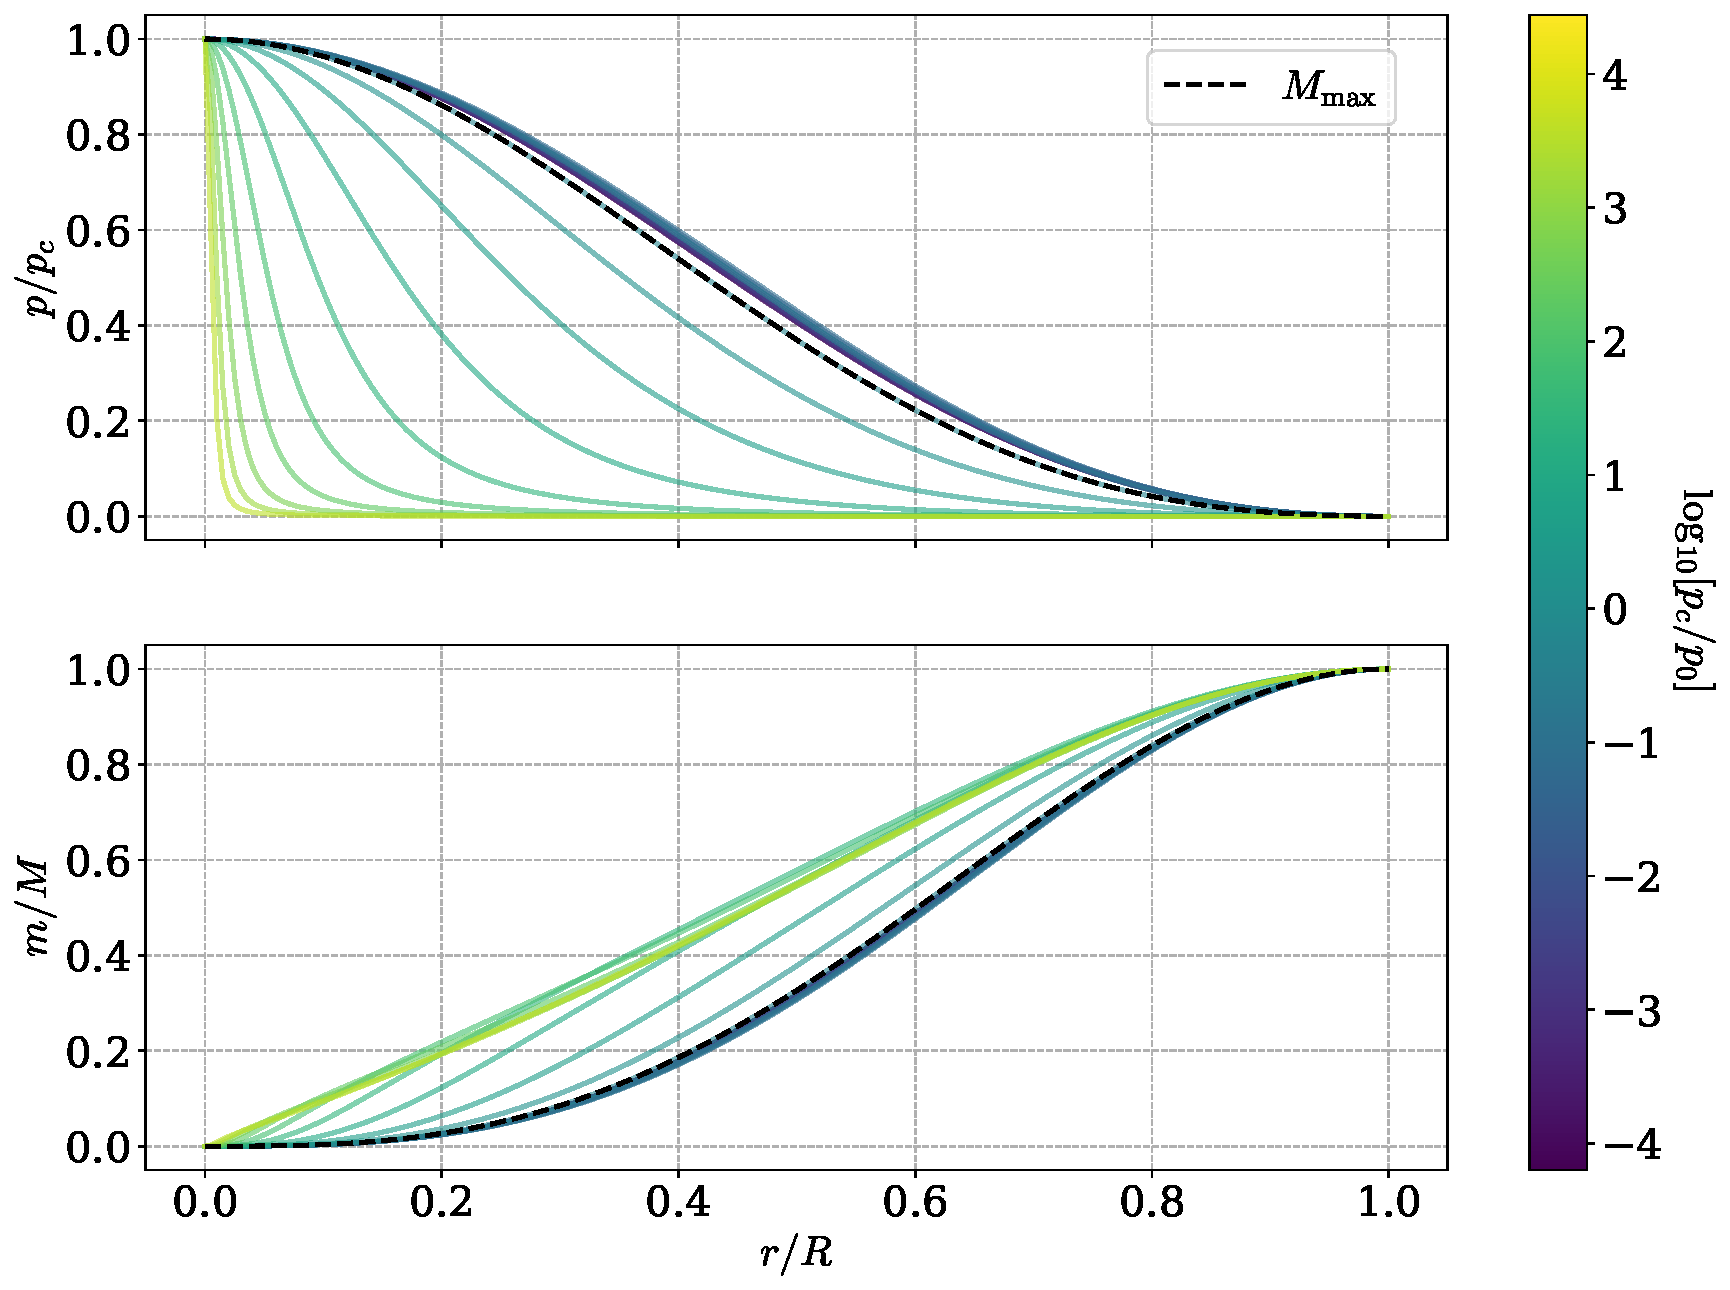
\includegraphics[width=0.8\textwidth]{../scripts/figurer/pion_star/pressure_mass_pion_star.pdf}
    \caption{
    Top: The pressure normalized to the central pressure, as a function of radius, normalized to the stellar radius.
    Bottom: The mass, normalized to the stellar mass, within a radius $r$, normalized to the stellar radius.
    Both plots show a range of stars with different central pressures, indicated by the color.
    The black dashed line corresponds to the star with the largest mass.
    }
    \label{fig: pressure and mass for pion star}
\end{figure}

\begin{figure}[!htb]
    \centering
    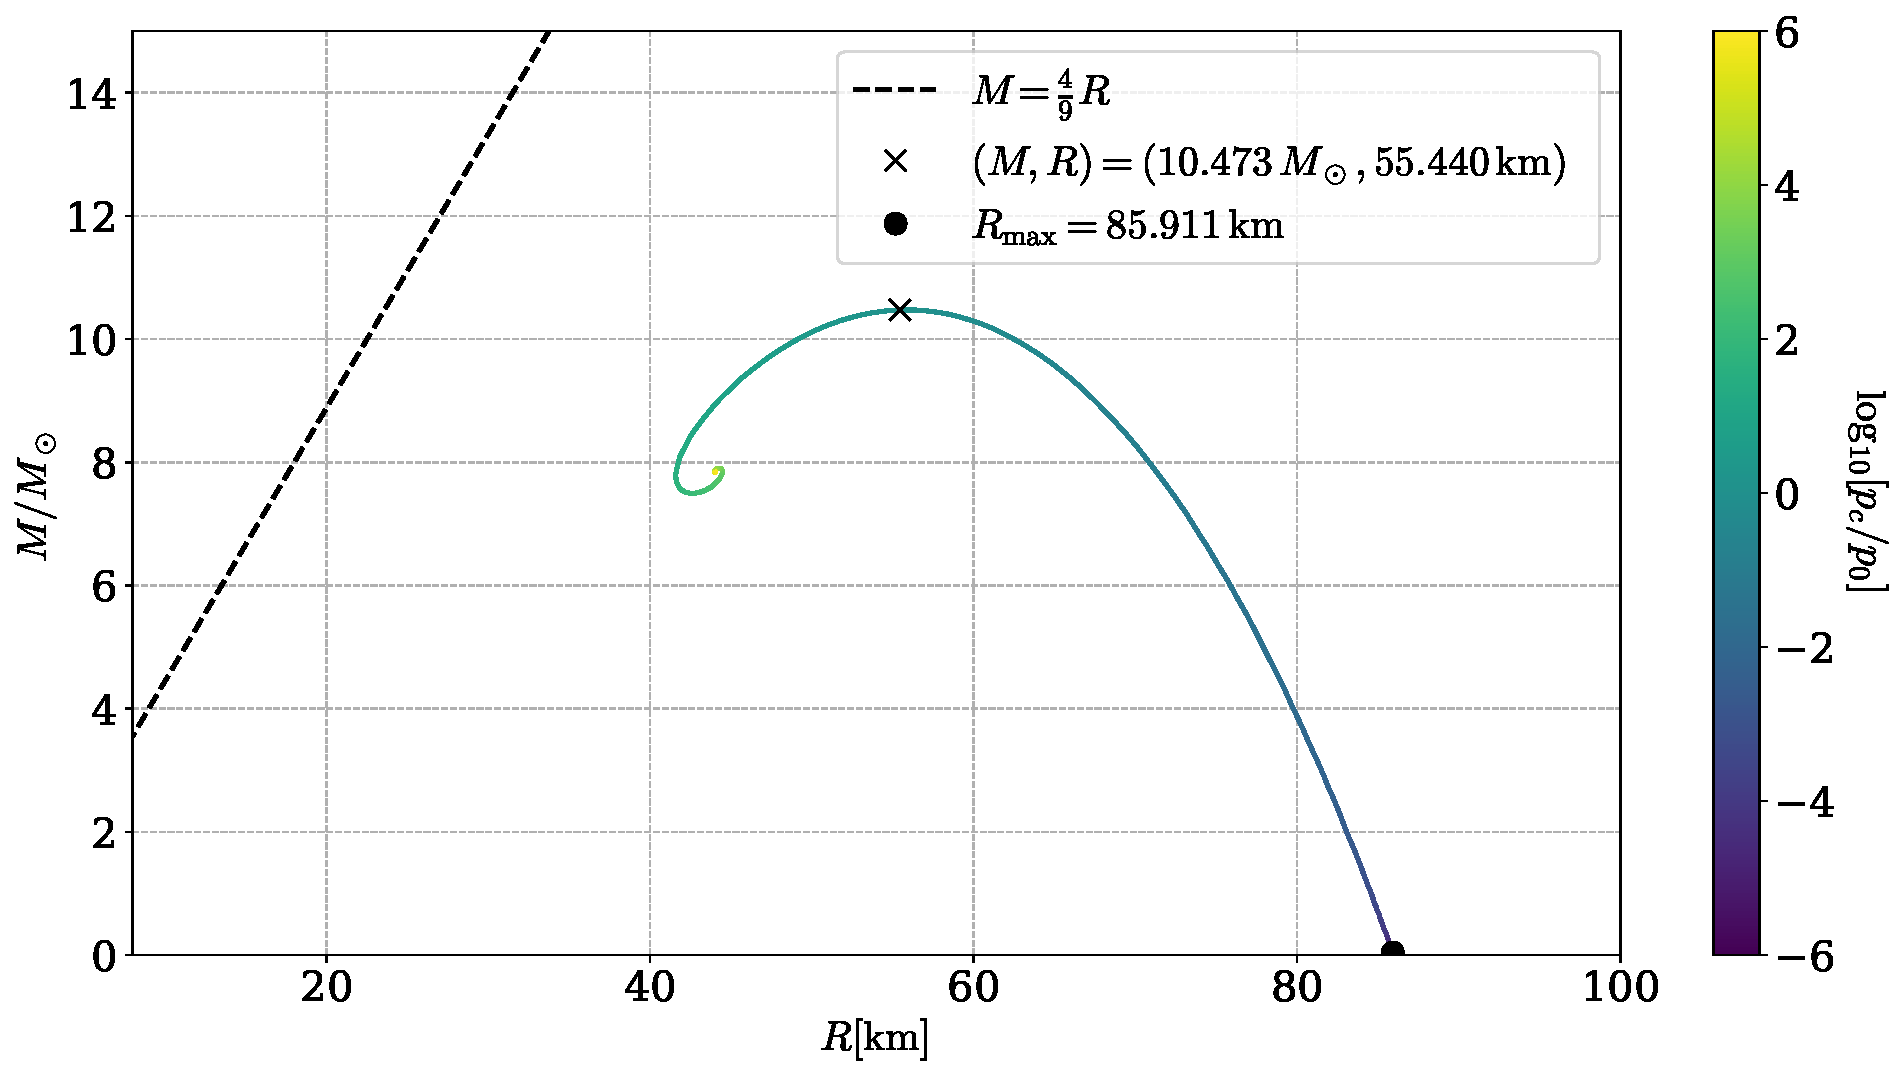
\includegraphics[width=0.85\textwidth]{../scripts/figurer/pion_star/mass_radius_pion_star.pdf}
    \caption{
        The lowest order mass-radius relation of a pion star using two-flavor chiral perturbation theory.
        The mass is given in units of solar masses, while the radius is measured in kilometers.
        This line is parameterized by the central pressure $p_c$ of the star, as indicated by the color gradient.
        The dashed black line indicates the theoretical maximum mass for a given radius, and any configuration above it will collapse to form a black hole.
        }
        \label{fig: mass-radius relation pion star}
\end{figure}

\begin{figure}[!htb]
    \centering
    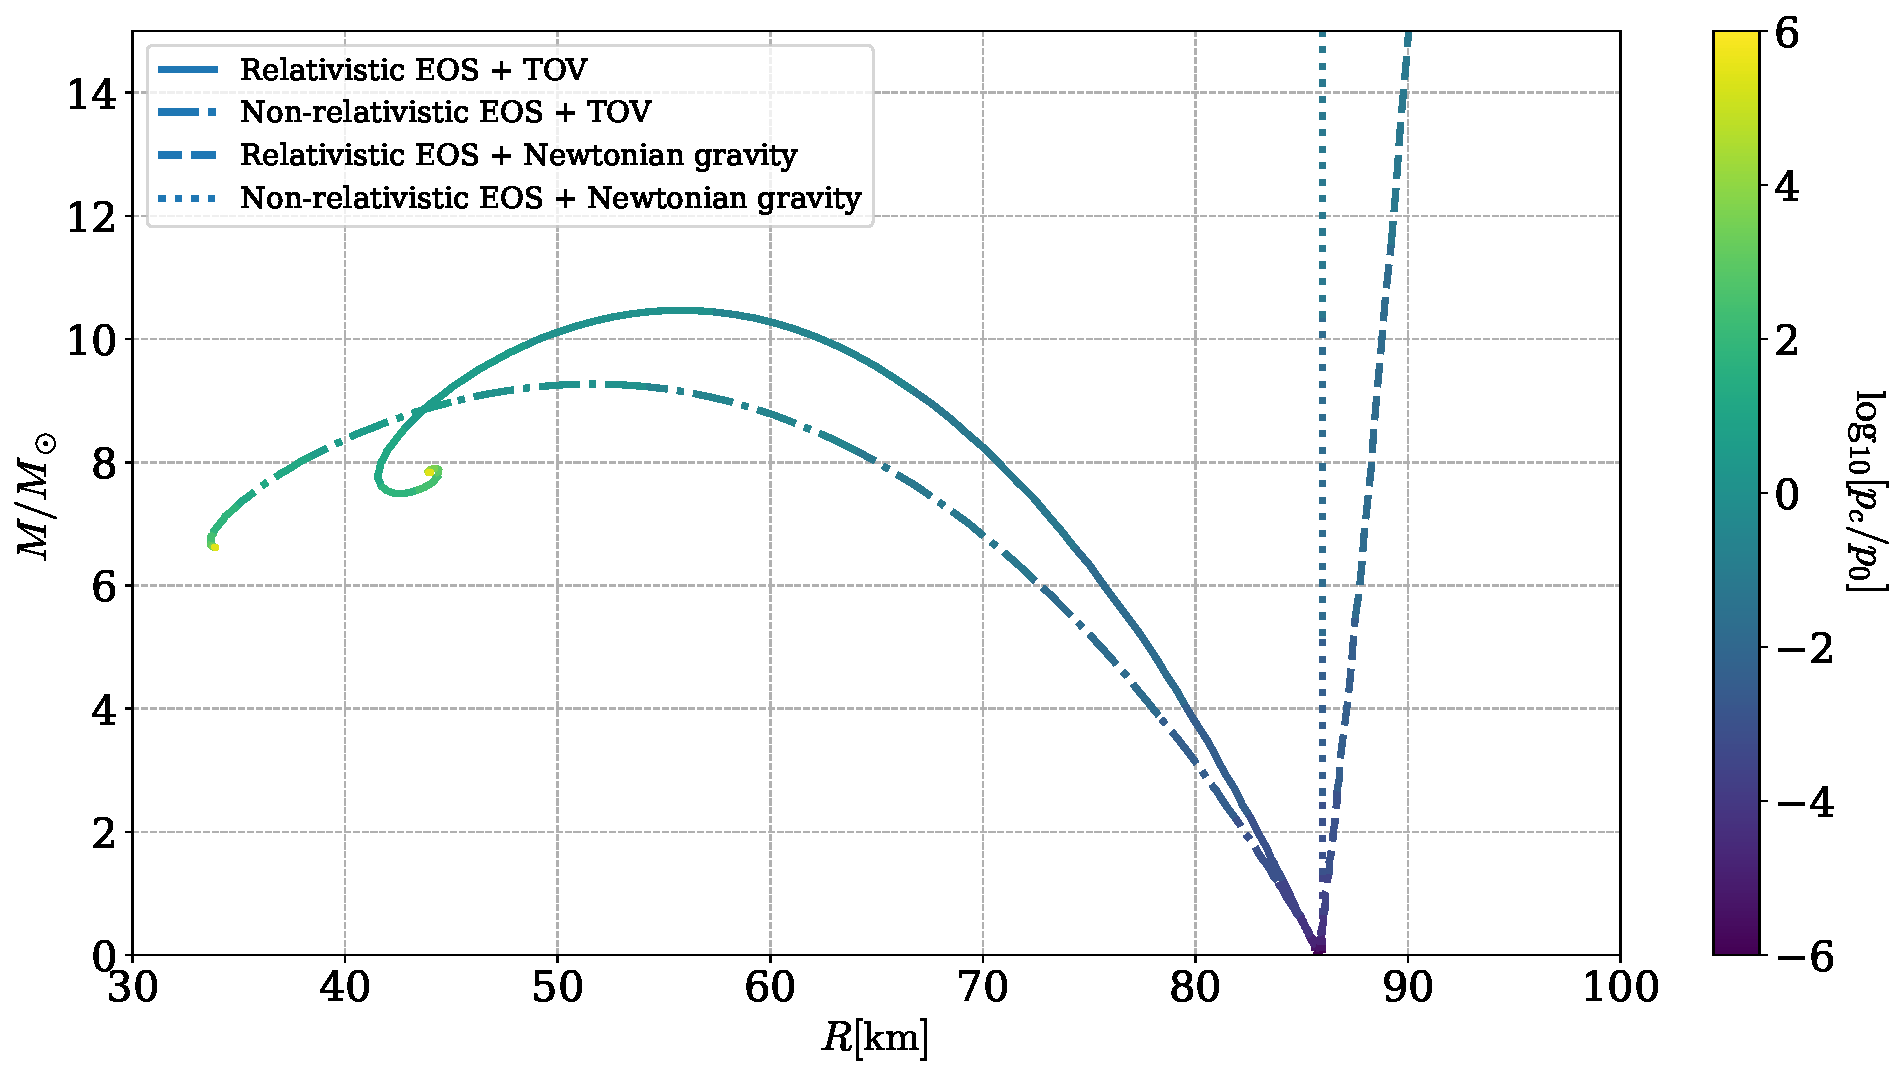
\includegraphics[width=0.85\textwidth]{../scripts/figurer/pion_star/mass_radius_comparison.pdf}
    \caption{
        The mass-radius relationship of the pion star from the full, leading-order equation of state from two-flavor chiral perturbation and the TOV equation, compared with results in various limits.
        }
        \label{fig: mass-radius relation pion star comparison}
\end{figure}



\FloatBarrier
\subsection{Including electromagnetic contributions}

As we found in \autoref{subsection: including electromagnetism lo eos}, the electromagnetic interaction of the pseudoscalar mesons contributes to the equation of state, even at leading order.
\autoref{fig: pressure and energy with EM interaction} shows the pressure and energy density, normalized to their characteristic quantities, as a function of chemical potential above the critical value, normalized to $\bar m$.
\autoref{fig: eos chpt em interaction} shows the equation of state.
The results with and without electromagnetic results are compared.
We see that the inclusion of electromagnetic contributions results in a less stiff equation of state; a given pressure corresponds to a higher energy density when including electromagnetic interactions.

\autoref{fig: mass-radius relation leading order pion star with em interaction} shows the mass-radius reaction of the pion star when the electromagnetic interaction is taken into account.
We see that the shape of the curve has not changed much from our earlier result. 
Both the maximum mass and radius are slightly smaller.
The new result for maximum radius, $R_\text{max} = 80.35 \, \text{km}$, is in excellent agreement with our expectation, \autoref{maximum mass pion star with em interaction}.
The result with and without electromagnetic interaction is compared in \autoref{fig: mass-radius relation comparison}.
As discussed in \autoref{section: cold fermi star}, we expect a stiffer equation of state to correspond to a more massive star, as happens in this case.

\begin{figure}[!htb]
    \centering
    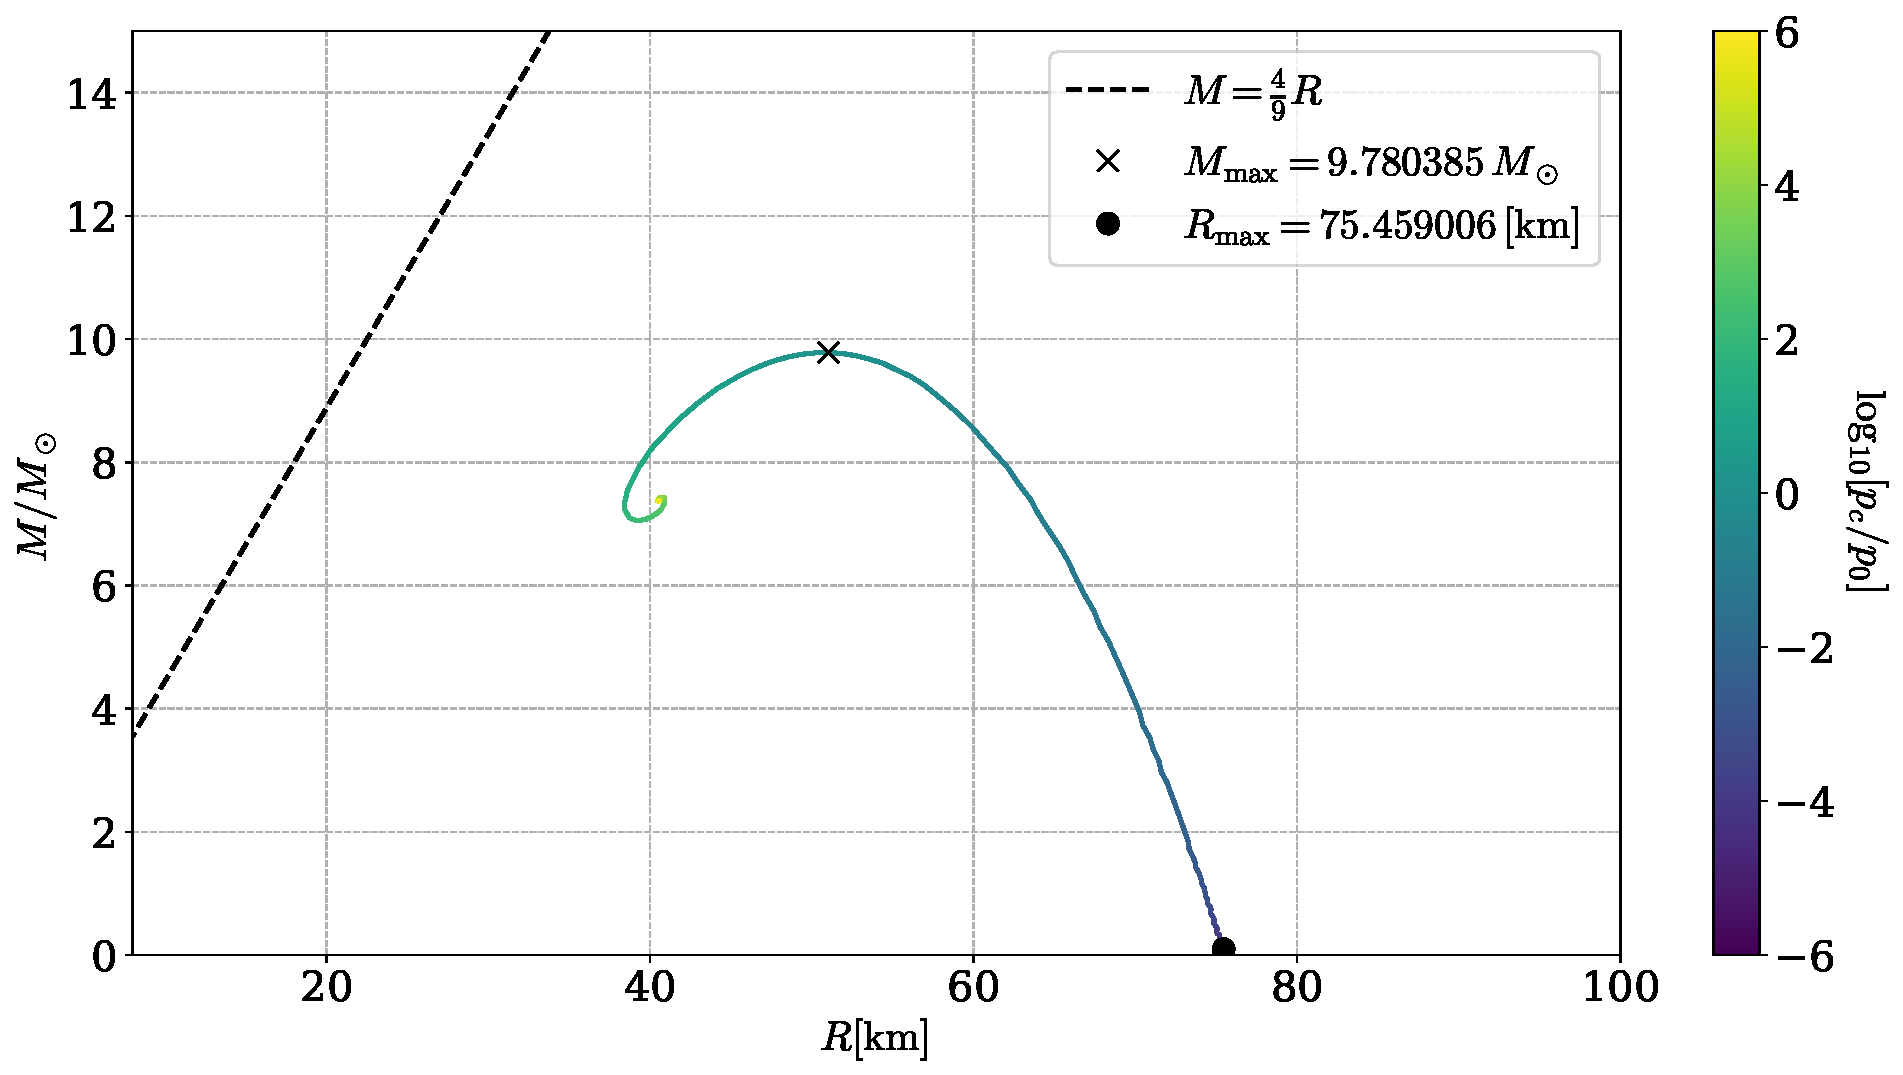
\includegraphics[width=0.85\textwidth]{../scripts/figurer/pion_star/mass_radius_pion_star_EM.pdf}
    \caption{
        The mass-radius relation of a pion star including electromagnetic interactions, parameterized by the logarithm of the central pressure.
        The dashed line shows the absolute limiting mass for a given radius.
        The cross indicates the maximum mass configuration, and the dot the maximum radius configuration.
        The mass is given in units of solar masses, while the radius is in kilometers.
        }
    \label{fig: mass-radius relation leading order pion star with em interaction}
\end{figure}


\begin{figure}[!htb]
    \centering
    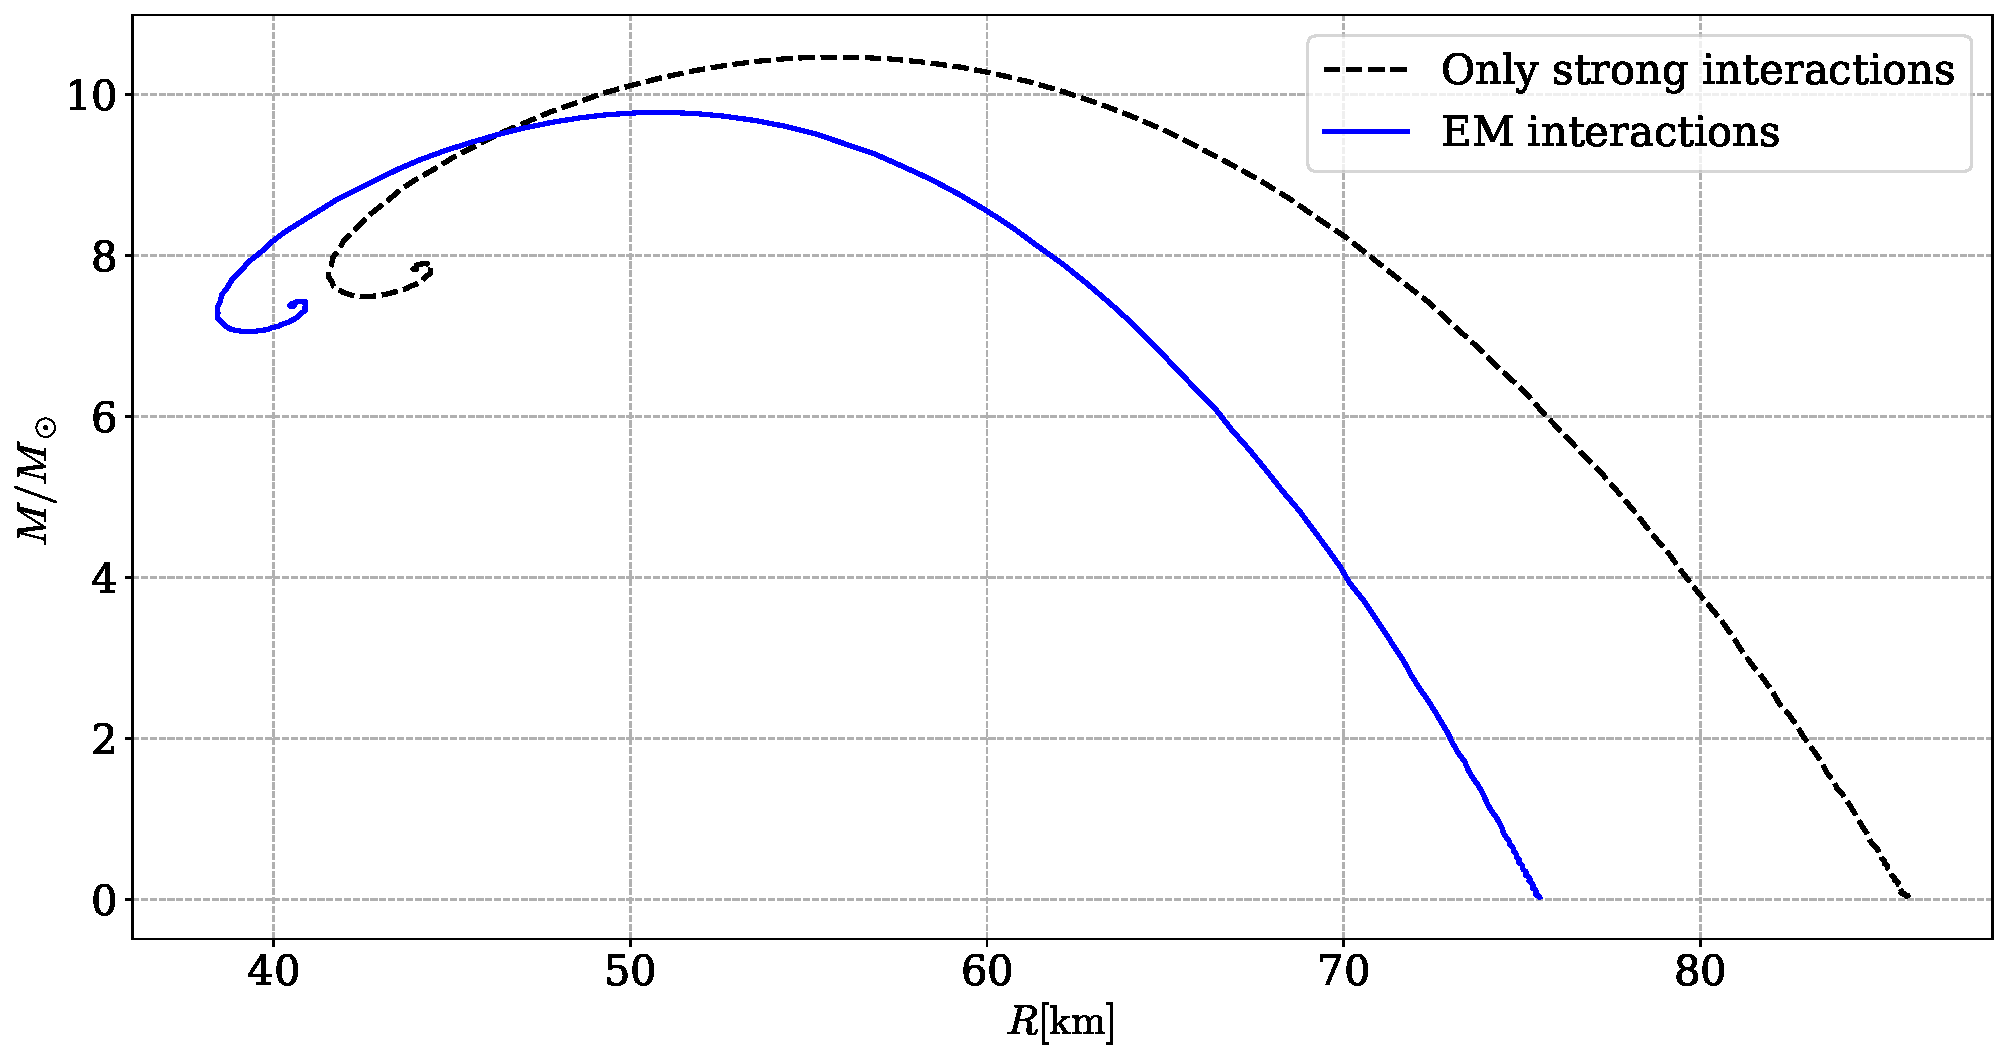
\includegraphics[width=0.8\textwidth]{../scripts/figurer/pion_star/mass_radius_pion_star_compare.pdf}
    \caption{
        The mass-radius relation of pion stars with and without the effects of electromagnetism included.
        The radius is given in kilometers and the mass in units of the solar mass.
        The marked points are the maximum mass and corresponding radius of the stars.
        }
        \label{fig: mass-radius relation comparison}
\end{figure}



\FloatBarrier
\subsection{Charge neutral stars}


We now apply the results from \autoref{section: charge neturality}, where we added a lepton to enforce charge neutrality.
As the electromagnetic force is long-range, we should expect any macroscopic astronomical object to be charge neutral.
First, we apply the system of pions and one charged lepton.
The star with electrons is shown in \autoref{fig: mass-radius relation with electrons}.
We see that this star is much larger than those made of only pions.
This is because the light electrons make the equation of state stiffer at low pressures.
The non-relativistic equation of state is now a polytrope with $\gamma = \frac{5}{3}$, instead of $\gamma = 2$, and there is, therefore, no upper limit on the radius.
The maximum mass is now $238\, M_\odot $, and the corresponding maximum radius is $ 3.11\times 10^4 \,\text{km}$.

The mass-radius relation for a star where the lepton is a muon is shown in \autoref{fig: mass-radius relation with muons}.
This has a similar form to that where the lepton was the electron, only smaller and lighter, as the equation of state, in this case, is less stiff.
The maximum mass is now $18.6\, M_\odot $, and the corresponding maximum radius is $ 262 \,\text{km}$.

\begin{figure}[!htb]
    \centering
    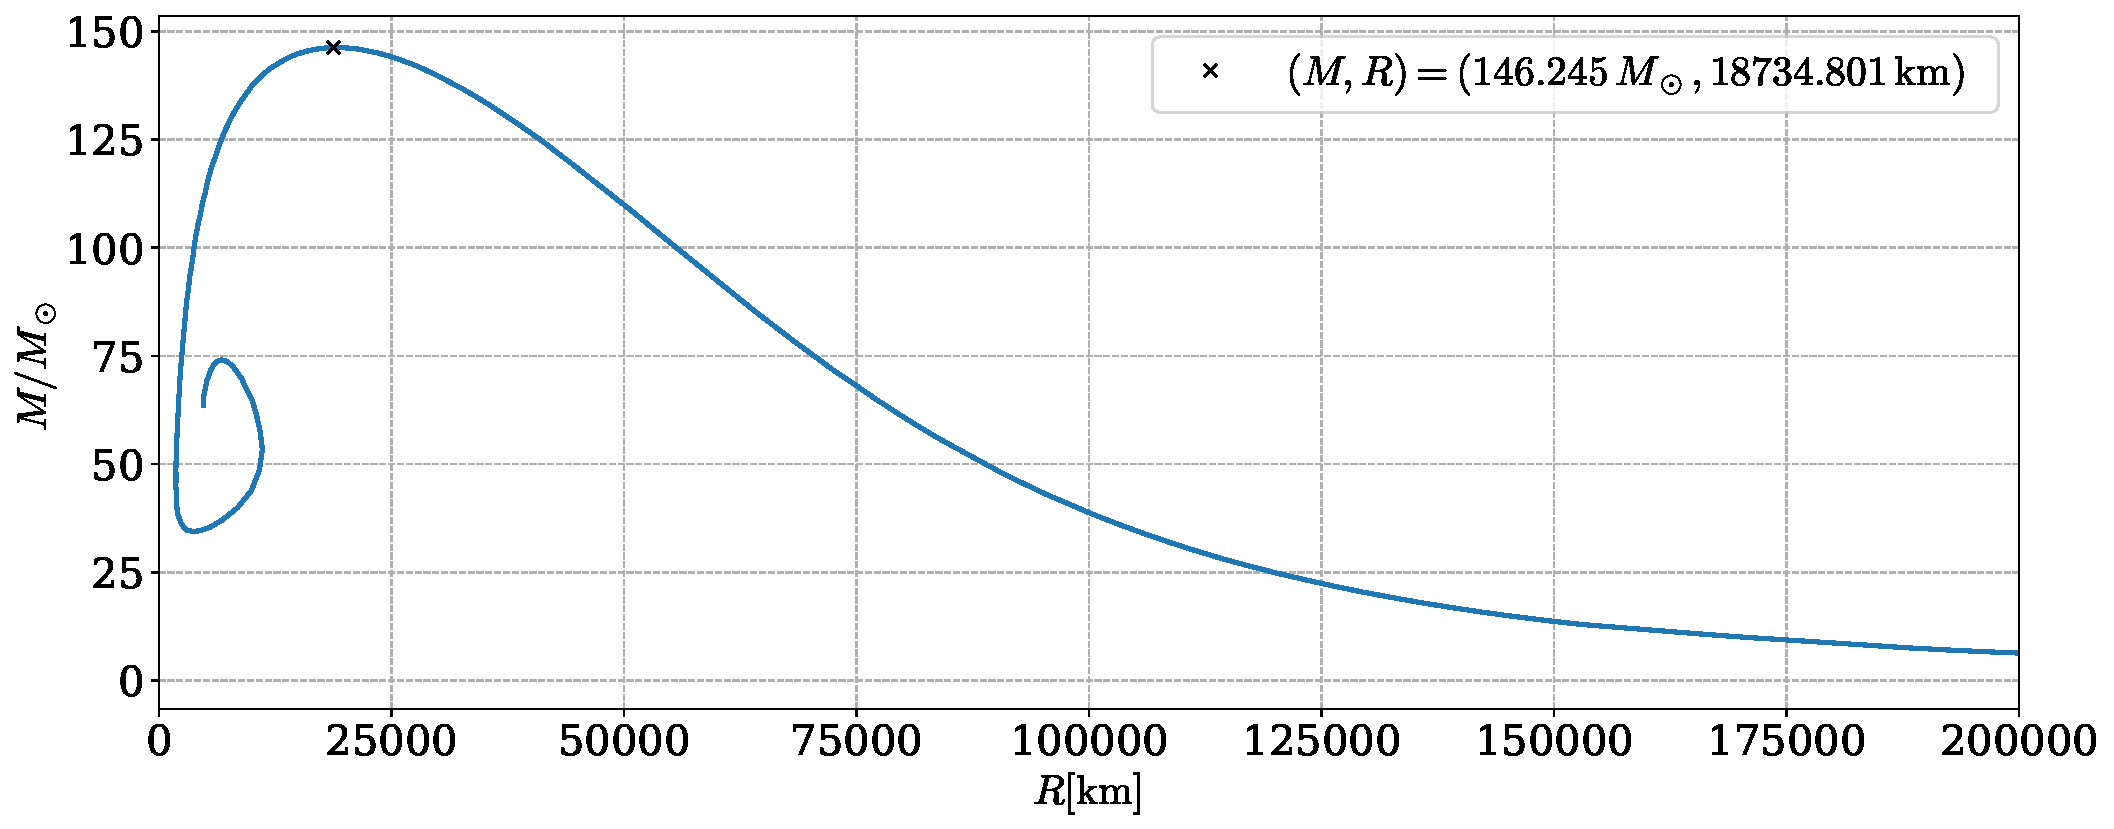
\includegraphics[width=\textwidth]{../scripts/figurer/pion_star/mass_radius__e.pdf}
    \caption{
        The mass-radius relation of pion stars with electrons enforcing charge neutrality.
        The radius is given in kilometers and the mass in units of solar masses.
        }
        \label{fig: mass-radius relation with electrons}
\end{figure}

\begin{figure}[!htb]
    \centering
    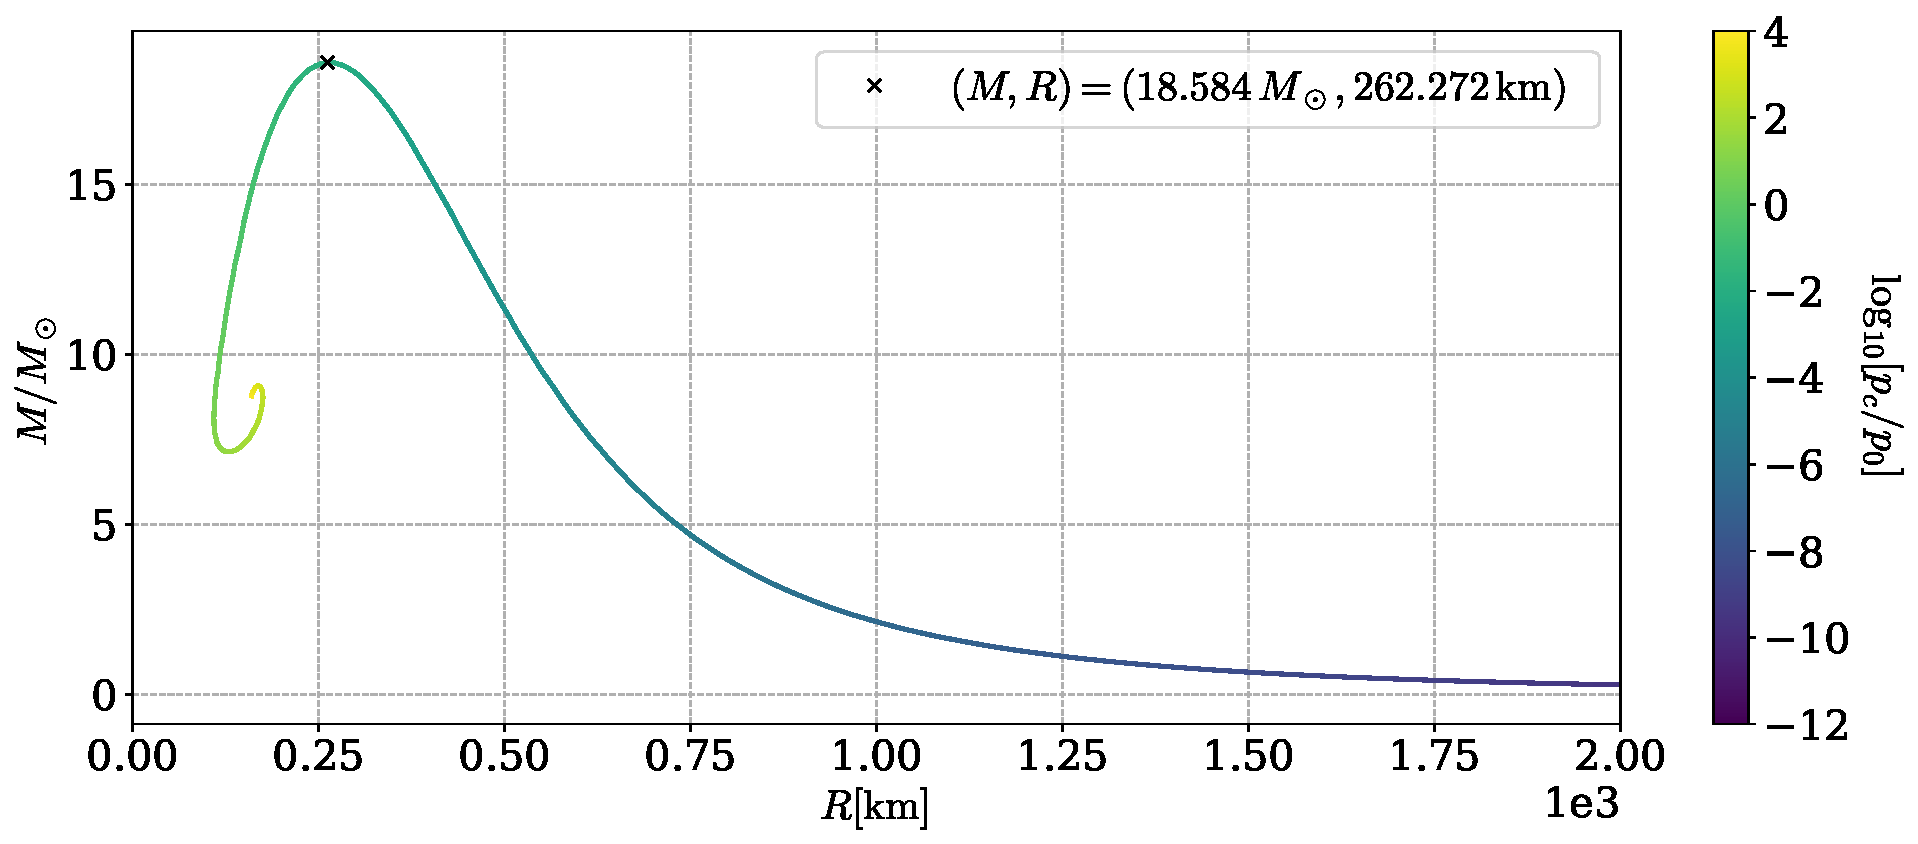
\includegraphics[width=\textwidth]{../scripts/figurer/pion_star/mass_radius__mu.pdf}
    \caption{
        The mass-radius relation of pion stars, including leptons to enforce charge neutrality, is compared with pion stars of only pions.
        The radius is given in kilometers and the mass in units of solar masses.
        }
        \label{fig: mass-radius relation with muons}
\end{figure}



\subsection{Neutrinos}

In \autoref{subsection: neutrinos}, we found the equation of state when including neutrinos in addition to charged leptons and the decay of pions due to the weak force.
In this case, the pressure and energy density do not vanish as the isospin density vanishes, but rather as $p = p_\text{min}>0$ as defined in \autoref{p min}
This is due to the contribution of neutrinos.
We therefore define the stellar radius $R$ by $p(R) = p_\text{min}$, where the pion condensate vanishes.
Such a star will therefore have an atmosphere of ultrarelativistic neutrinos.
For $p < p_\text{min}$, the equation of state is that of massless fermions and will therefore not have a finite radius.
There is a $p+u$-term on the right-hand side of the TOV equation, \autoref{TOV}.
When we defined the stellar radius by $p(R) = 0$, this factor vanishes as we approach the surface of the star, while now $p+u \geq 4 p_\text{min}$.
Close to the surface, the pressure will therefore fall faster, as a consequence of $p_\text{min}>0$.
The resulting mass-radius relation is shown in \autoref{fig: mass radius neutrino}.
We see that, in contrast to the earlier results, both the mass and radius approach zero as $p_c \rightarrow p_\text{min}$.


\begin{figure}[!htb]
    \centering
    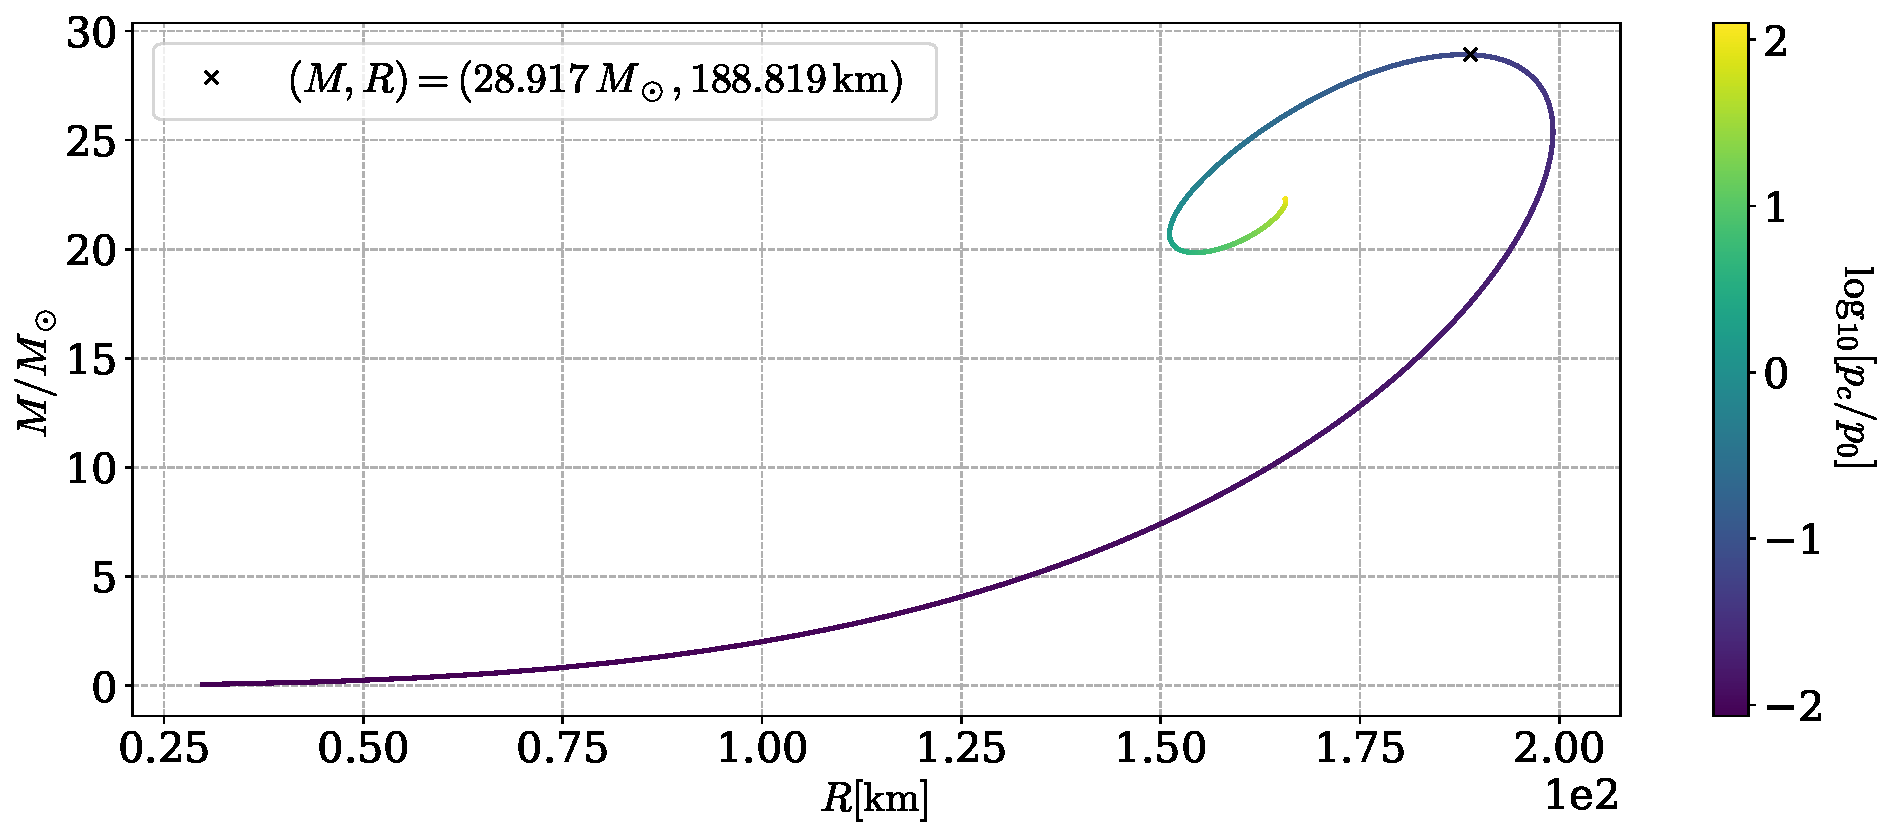
\includegraphics[width=\textwidth]{../scripts/figurer/pion_star/mass_radius_neutrino.pdf}
    \caption{
        The mass-radius relation of pion stars, including leptons and neutrinos in equilibrium.
        The radius is given in kilometers and the mass in units of solar masses.
        }
        \label{fig: mass radius neutrino}
\end{figure}

In \autoref{fig: light stars}, the pion stars including charged leptons and neutrinos are compared to a family of stars with $u = 3p$ but different values for $p_\text{min}$.
We see that the mass-radius relation of the pion star closely resembles that of such a star and that the mass-radius relationship, therefore, is mostly set by $p_\text{min}$.


\begin{figure}[!htb]
    \centering
    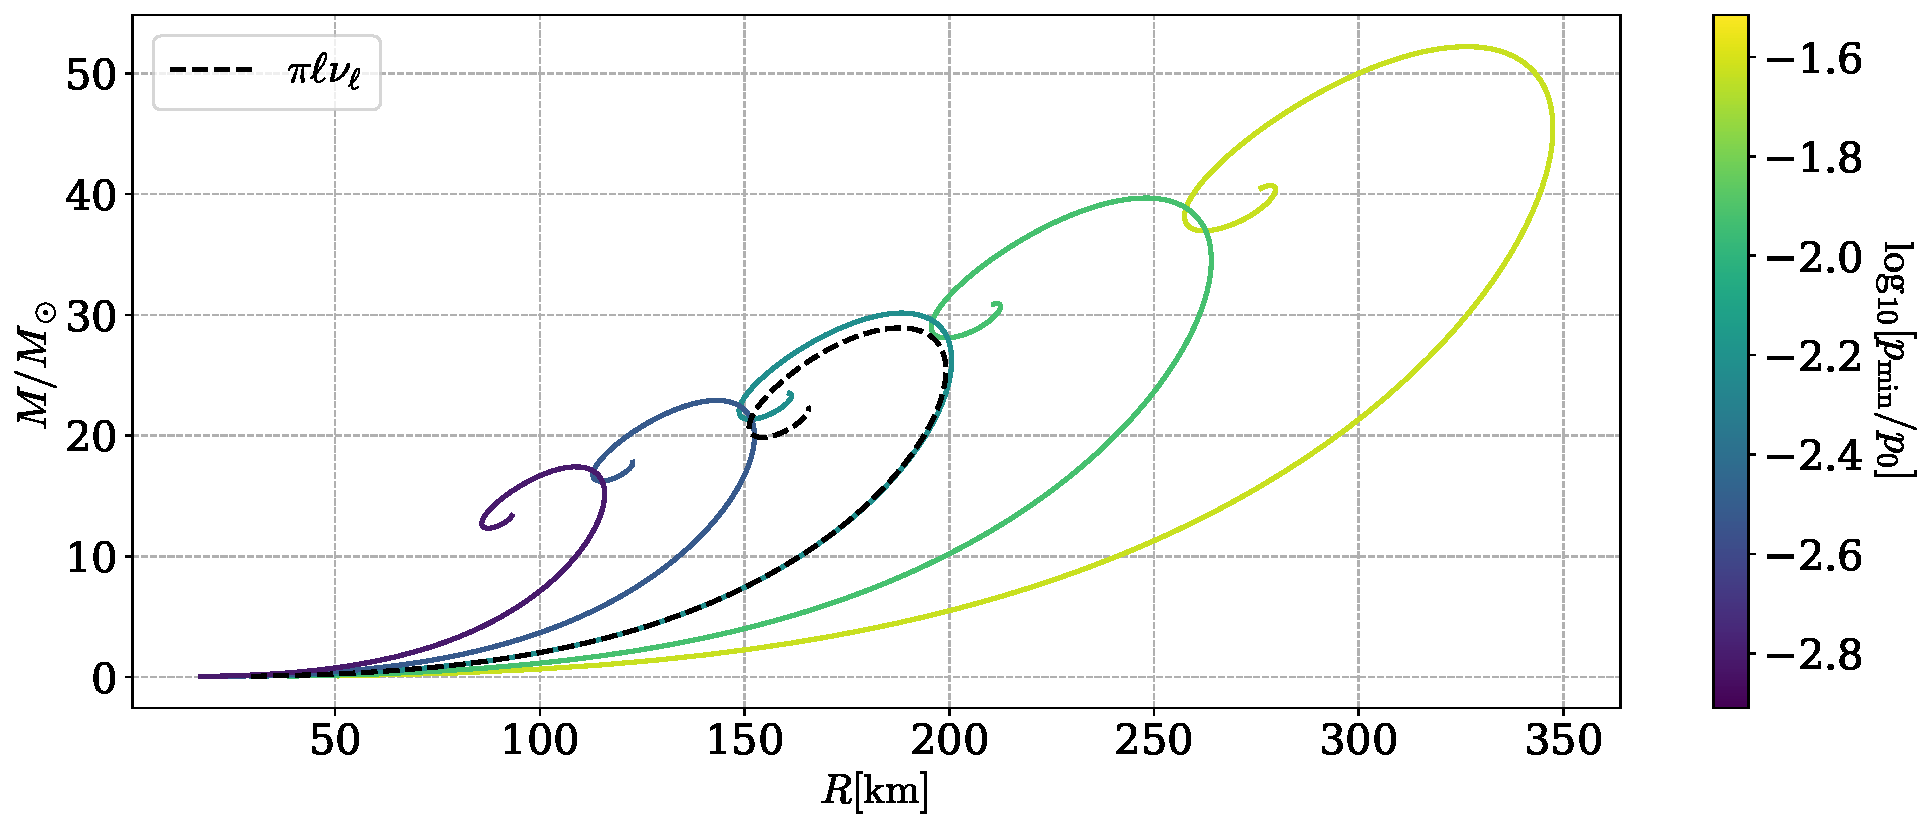
\includegraphics[width=\textwidth]{../scripts/figurer/pion_star/mass_radius_light.pdf}
    \caption{Stars with equation of state $u = 3p$ but different values for $p_\text{min}>0$ is compared to the pion star with charged leptons and neutrinos.}
    \label{fig: light stars}
\end{figure}


\subsection{NLO pion star}

We now use the next-to-leading order results for the pure pion condensate, which we found in \autoref{section: nlo thermodynamics}.
The mass-radius relationship, in this case, is shown in \autoref{fig: mass-radius relation nlo}.
The maximum mass is $M_\text{max} = 9.94\, M_0$, and the corresponding radius is $R = 54.09\,\text{km}$.
In \autoref{fig: mass-radius relation compare nlo}, we compare the leading order and next-to-leading order mass-radius relations.
The results are similar, however, the next-to-leading order star is smaller and less massive, as is expected for a less stiff equation of state.

\begin{figure}[!htb]
    \centering
    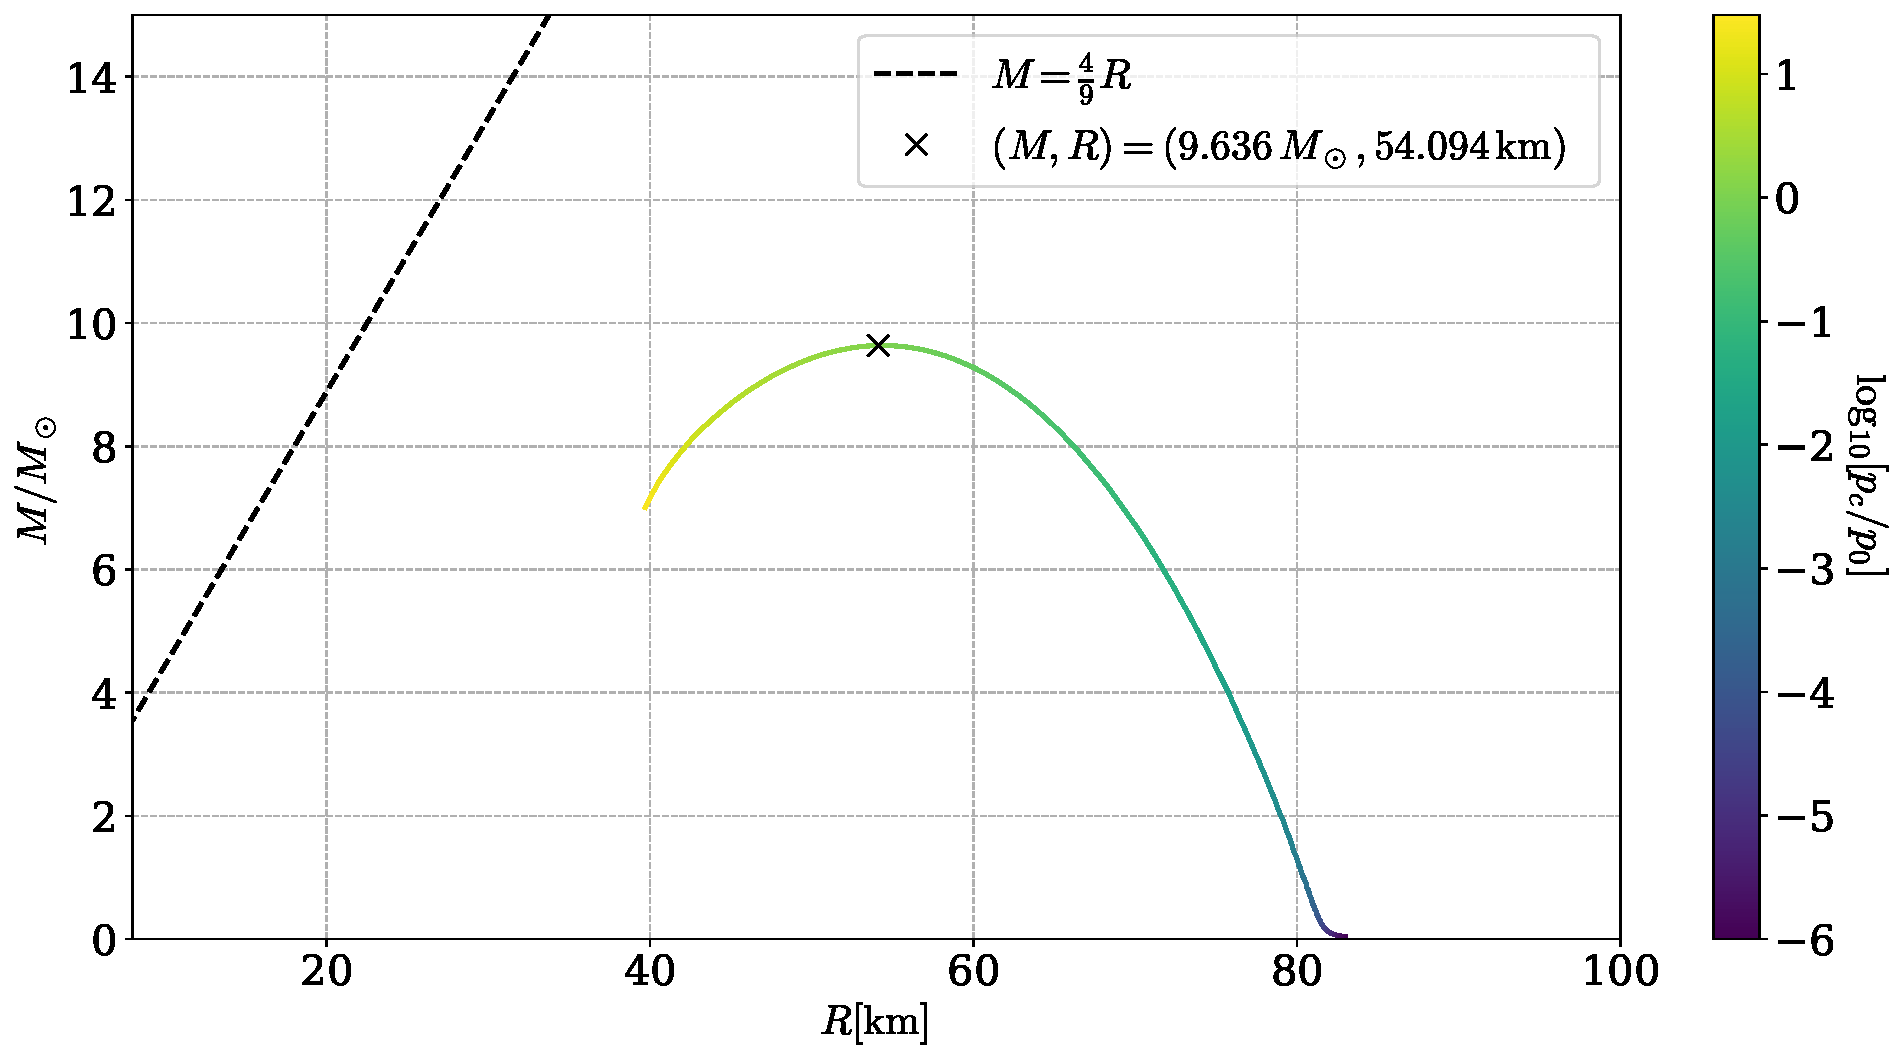
\includegraphics[width=\textwidth]{../scripts/figurer/pion_star/mass_radius_pion_star_nlo.pdf}
    \caption{The mass-radius relation of a pion star with the next-to-leading order equation of state.}
    \label{fig: mass-radius relation nlo}
\end{figure}

\begin{figure}[!htb]
    \centering
    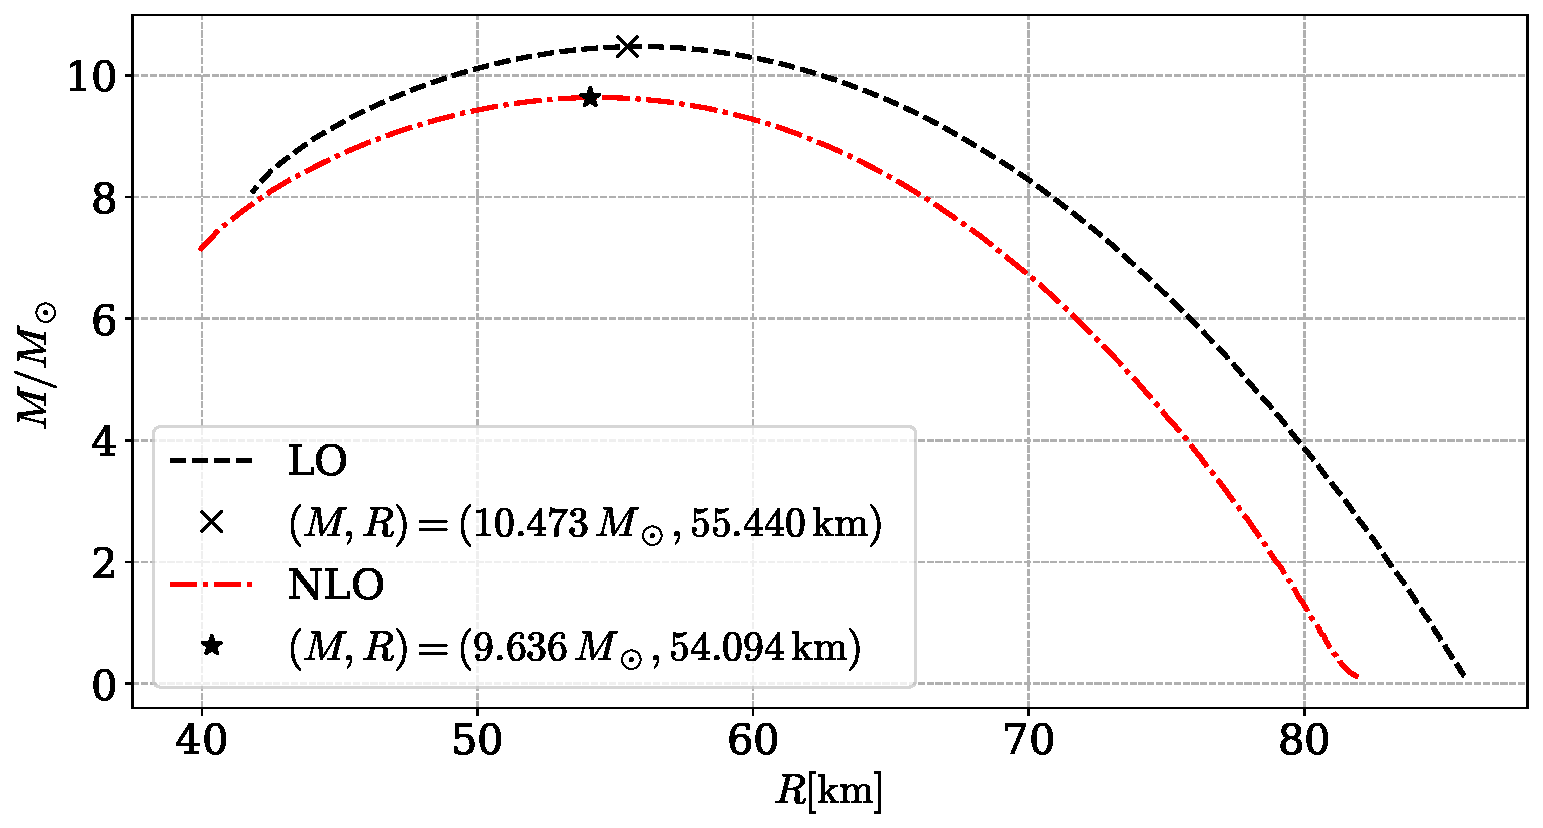
\includegraphics[width=\textwidth]{../scripts/figurer/pion_star/mass_compare_order.pdf}
    \caption{
        The mass-radius relation of a pion star using the leading and next-to-leading order equation of state is compared. 
        The mass is given in solar masses and the radius in kilometers.}
    \label{fig: mass-radius relation compare nlo}
\end{figure}



\section{Comparison and key values}



All results are compared in \autoref{fig: mass-radius relation with leptons}.

\begin{figure}[!htb]
    \centering
    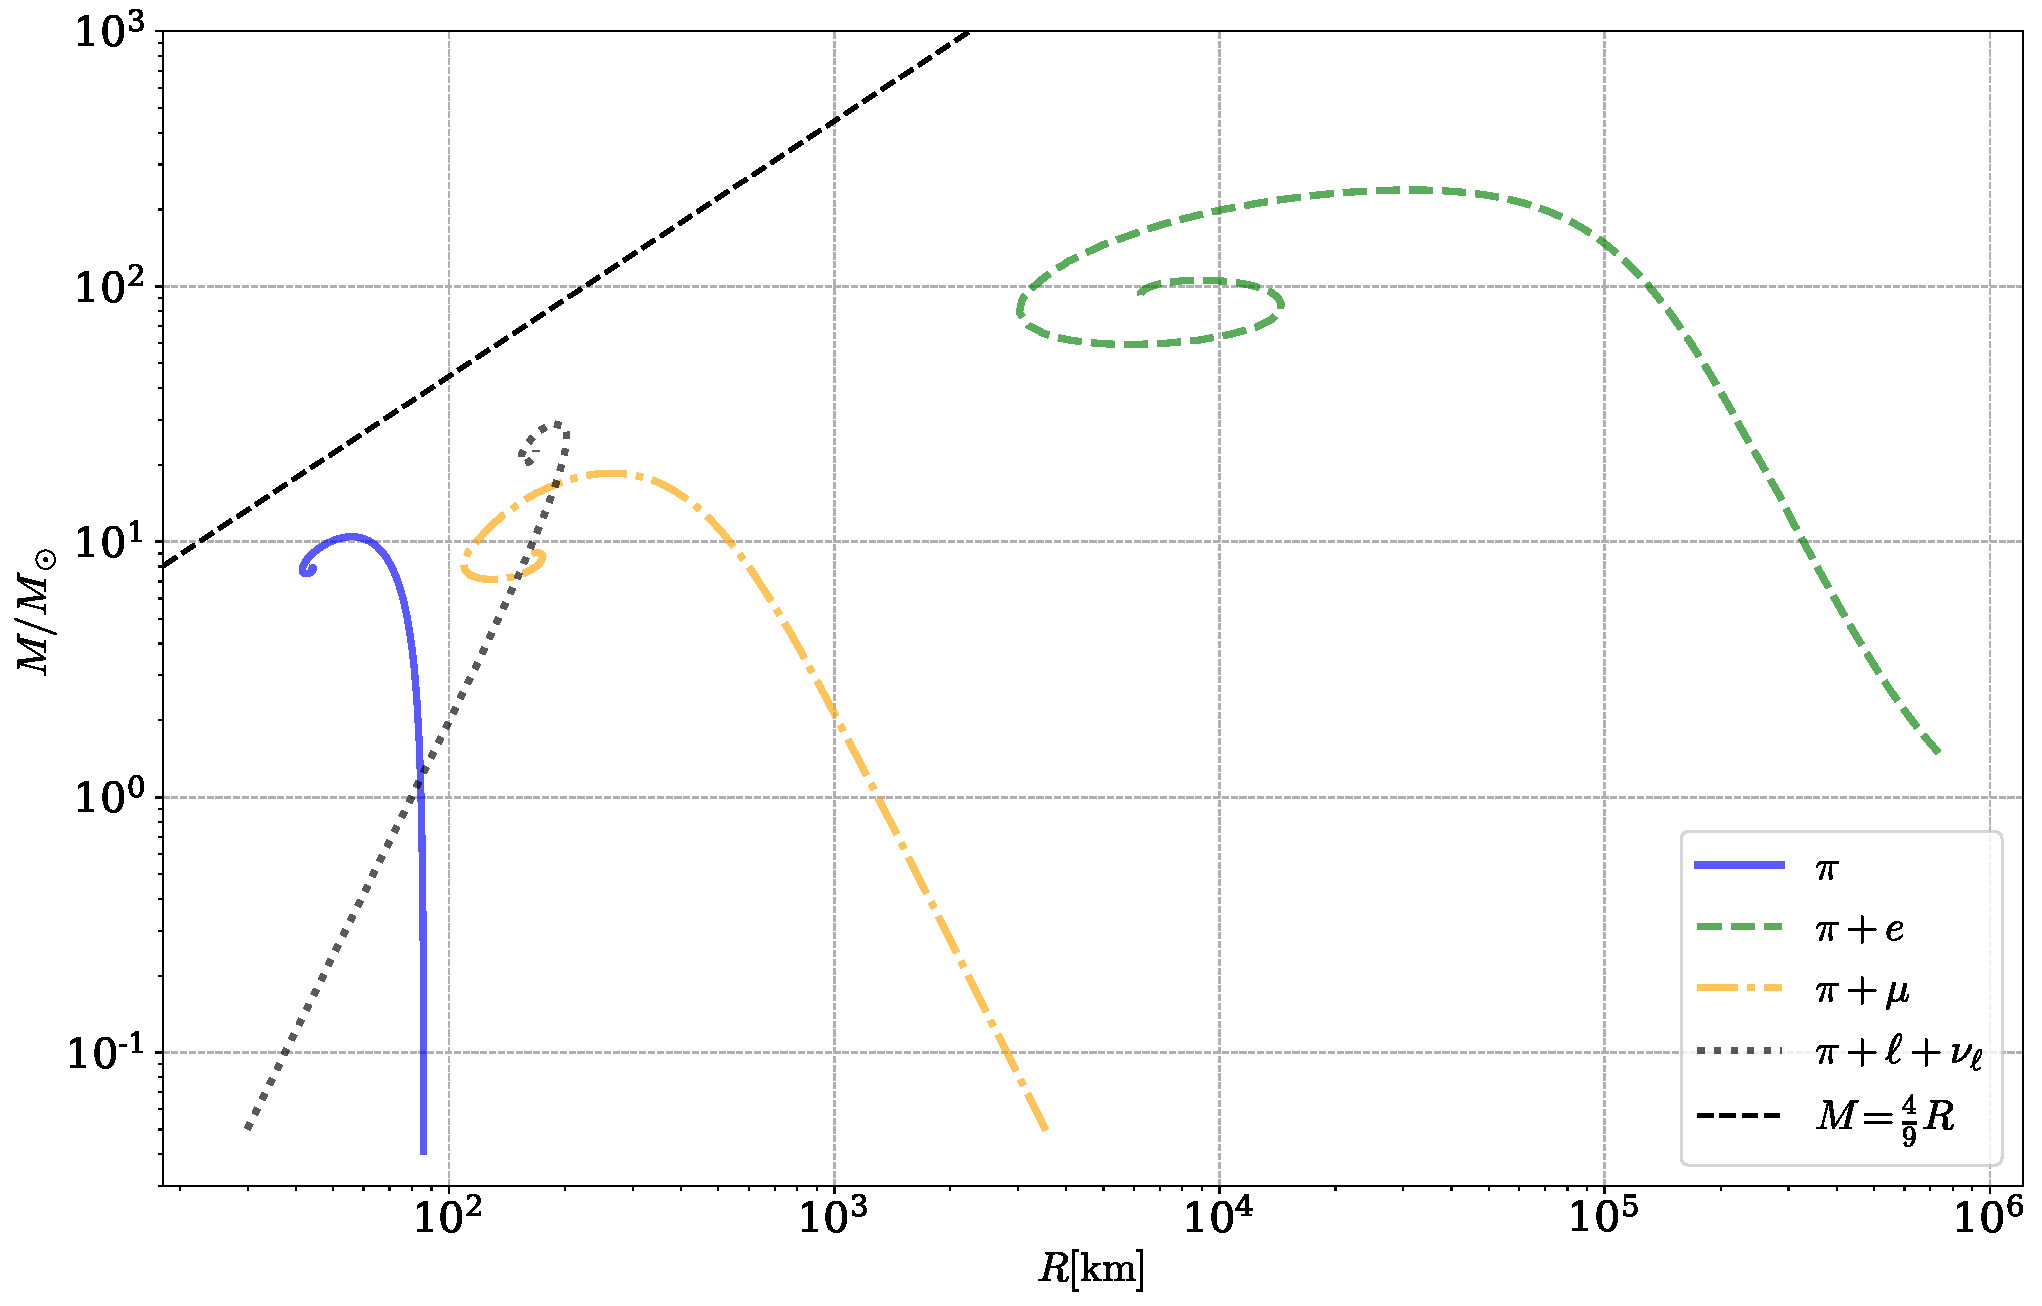
\includegraphics[width=\textwidth]{../scripts/figurer/pion_star/mass_radius_all.pdf}
    \caption{
        The mass-radius relation of pion stars, including leptons to enforce charge neutrality, is compared with pion stars of only pions.
        The radius is given in kilometers and the mass in units of solar masses.
        }
        \label{fig: mass-radius relation with leptons}
\end{figure}


Key values for each system are shown in \autoref{table: key values}.


\begin{table}[!htb]
    \centering
    \caption{The values of various quantities for the maximum mass stars}
    \label{table: key values}
    \begin{tabular}{c  c  c  c  c c c}
        \hline \hline
        system & $M_\text{max}/M_\odot$ & $R / \text{km}$ & 
        $u/u_0$ & $p/u_0$ & $\mu_I/m_\pi-1$ & $\mu_\ell/m_\ell-1$ \\
        \hline
        $\pi\,\, \text{LO}$& 10.47 & 55.38 & 2.864 & 1.318 & 0.8461& \\
        $\pi\, \text{NLO}$& 9.04 & 54.09 & 3.020 & 1.139 & 0.9256 & \\
        $\pi\,\,\text{EM}$& 10.11 & 53.58 & 2.930 & 1.318 & 0.8463 & \\
        $\pi + e$& 283.8 & 3.171$\times10^4$ & 
        2.550$\times10^{-6}$ & 1.995$\times10^{-8}$ & 
        6.222$\times10^{-6}$ & \\
        $\pi + \mu$& 18.58 & 262.3 & 
        0.1411 & 1.202$\times 10^{-2}$ &
        1.732$\times10^{-2}$& \\
        $\pi + \ell + \nu_\ell$& 28.92 & 188.8 &
        0.2262  & 6.847$\times 10^{-2}$ &
        5.264$\times10^{-3}$& \\
        \hline
    \end{tabular}
\end{table}



\subsection{Comparison with numerical results}

In \autocite{brandtNewClassCompact2018}, \citeauthor{brandtNewClassCompact2018} used the equation of state obtained by QCD lattice methods to obtain mass-radius relations for pion stars, with and without leptons for charge neutrality.
Their results are compared with ours in  \autoref{fig: brandt mass-radius}.


\begin{figure}[!htb]
    \centering
    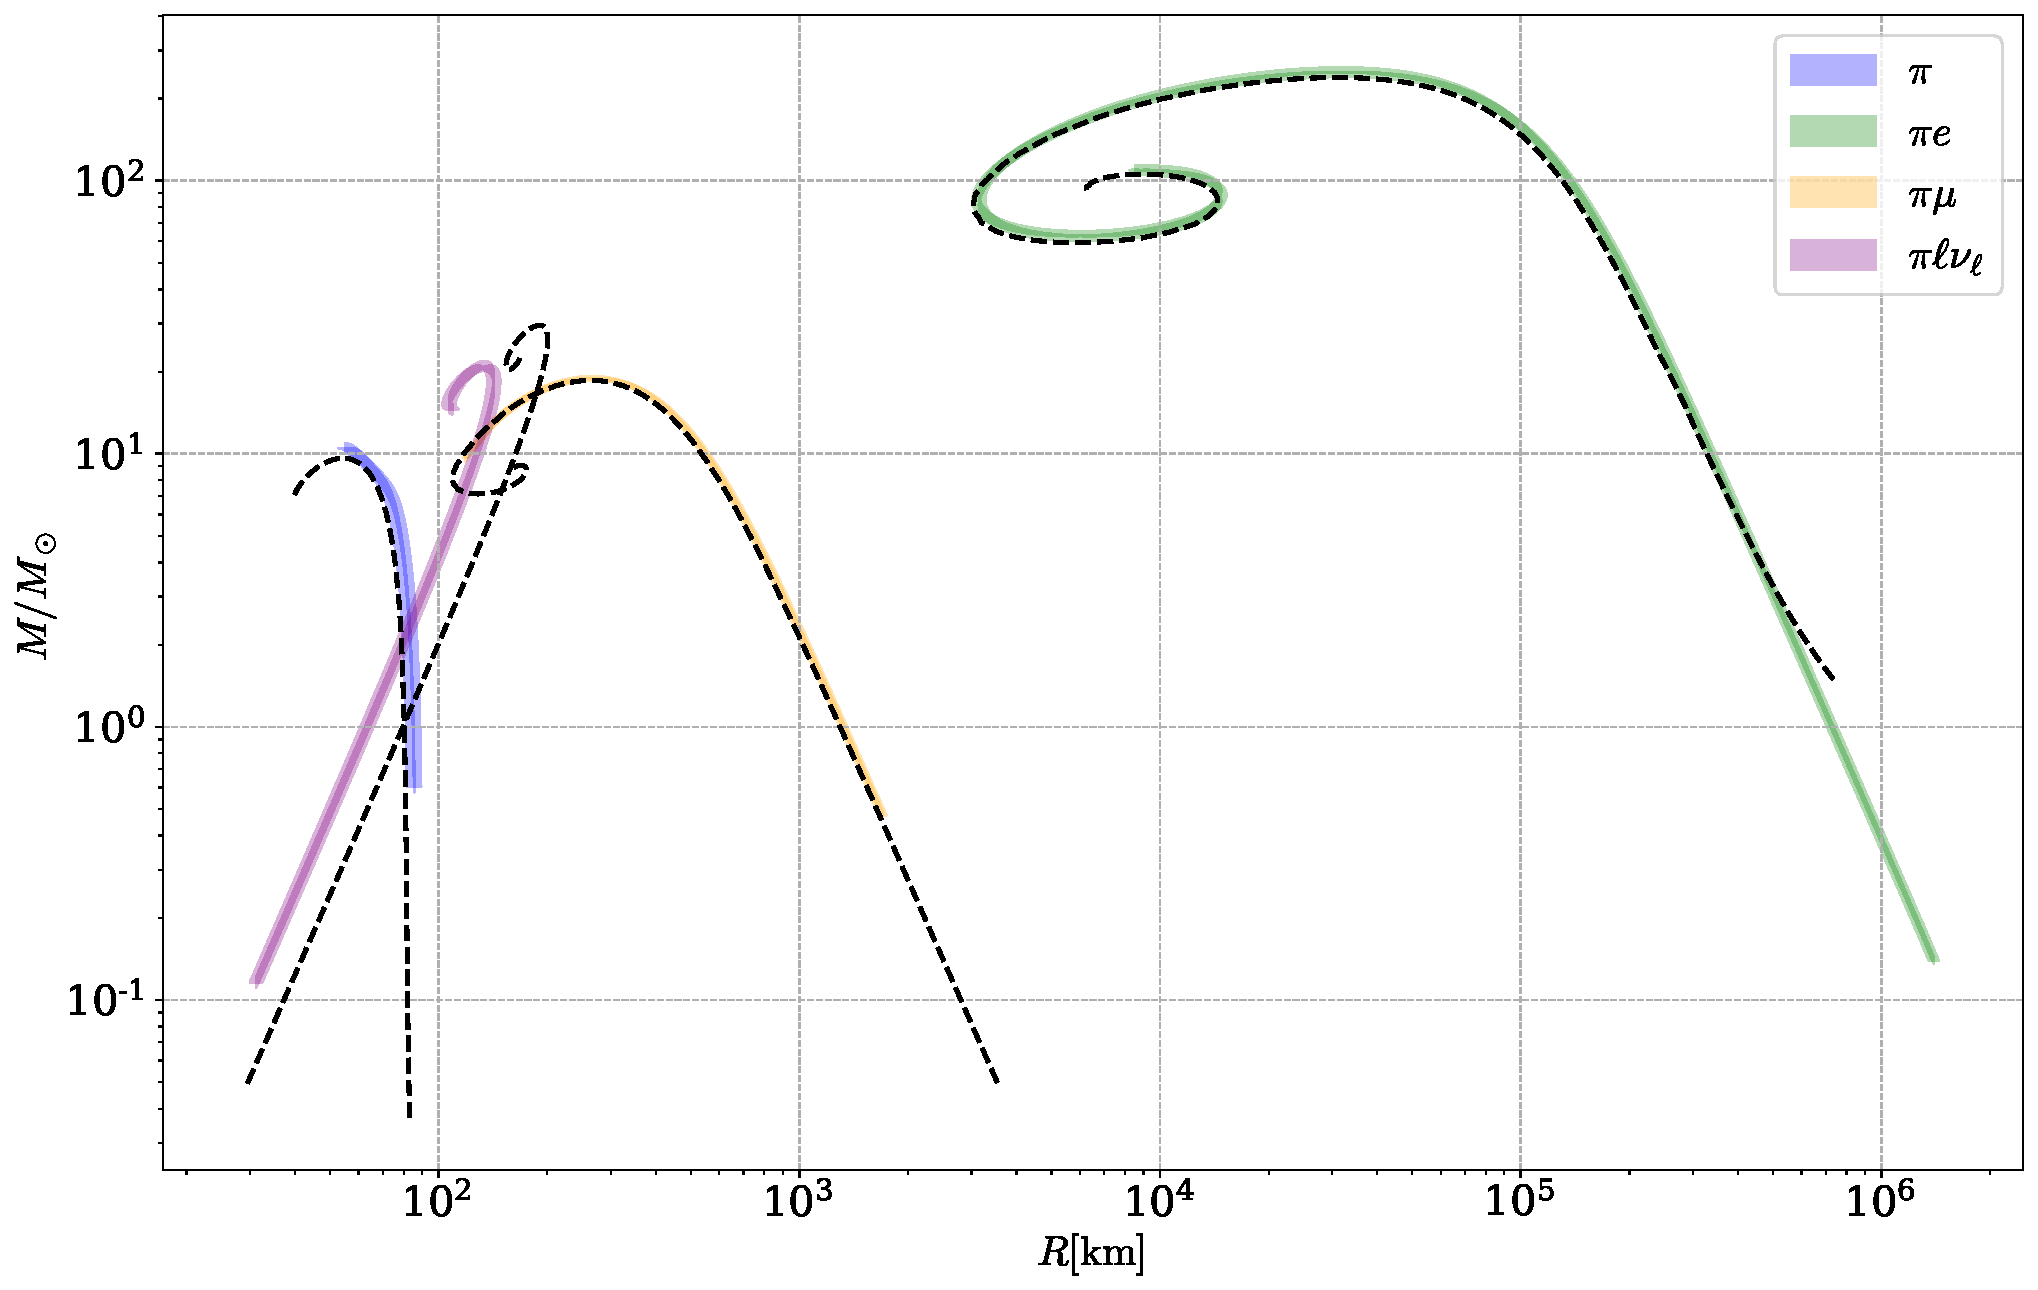
\includegraphics[width=\textwidth]{../scripts/figurer/pion_star/mass_radius_brandt_all.pdf}
    \caption{
        The mass-radius relations for pion stars, with and without leptons included.
        The results of \citeauthor{brandtNewClassCompact2018}, solid color, are compared with our results, dashed lines.
        The result of \citeauthor{brandtNewClassCompact2018} incorporate statistical and systematic uncertainty in both $R$ and $M$ in the width of the lines.
        The radius is in units of $\text{km}$, while mass are in solar masses, $M_\odot$.
    }
    \label{fig: brandt mass-radius}
\end{figure}



    \appendix

    \chapter[Appendix A]{}
    \section{Functionals}
\label{appendix: Functional derivatives}


The principle of stationary action and the path integral method relies on functional calculus, where ordinary, $n$-dimensional calculus is generalized to an infinite-dimensional calculus on a space of functions.
A functional, $S$, takes in a function $\varphi(x)$, and returns a real number $S[\varphi]$.
We will be often be dealing with functionals of the form
%
\begin{equation}
    \label{general action functional}
    S[\varphi] = \int_\Em \dd^n x \, \Ell[\varphi](x),
\end{equation}
%
Here, $\Ell[\varphi](x)$, the Lagrangian density, is a functional which takes in a function $\varphi$, and returns a real number $\Ell[\varphi](x)$ \emph{for each point} $x \in \Em$.
$\Ell$ thus return a real-valued function, not just a number.
$\Em$ is the manifold, in our case space-time, of which both $\varphi(x)$ and $\Ell[\varphi](x)$ are functions.
The function $\varphi$ can, in general, take on the value of a scalar, complex number, spinor, vector, etc\dots, while $\Ell[\varphi](x)$ must be a scalar-valued function.
This strongly constraints the form of any Lagrangian and is an essential tool in constructing quantum field theories.
Although this section is written with a single scalar-valued function $\varphi$, this can easily be generalized by adding an index, $\varphi \rightarrow \varphi_\alpha$, enumerating all the degrees of freedom, then summing over this index when restating the arguments~\autocite{carrollSpacetimeGeometryIntroduction2019,schwartzQuantumFieldTheory2013,peskinIntroductionQuantumField1995}.



\subsection{Functional derivative}

The functional derivative is base on an arbitrary \emph{variation} $\eta$ of the function $\varphi$.
The variation $\eta$, often written $\delta \varphi$ is an arbitrary function only constrained to vanish \emph{quickly enough} at the boundary $\partial \Em$.\footnote{%
The condition of ``quickly enough'' is to ensure that we can integrate by parts and ignore the boundary condition, which we will do without remorse.
}
The variation of the functional $S$ is defined as
%
\begin{equation}
    \delta_\eta S[\varphi] = \lim_{\epsilon \rightarrow 0} \frac{1}{\epsilon}
    \left( S[\varphi + \epsilon \eta] - S[\varphi] \right) 
    = \odv{}{\epsilon} S[\varphi + \epsilon \eta] |_{\epsilon = 0}.
\end{equation}
%
We can regard the variation of a functional as the generalization of the differential of a function, \autoref{covectors i.e. one forms}, as the best linear approximation around a point.
In regular differential geometry, a function $f$ can be approximated around a point $x$ by
%
\begin{equation}
    f(x + \epsilon v) = f(x) + \epsilon \dd f(v),
\end{equation}
%
where $v$ is a vector in the tangent space at $x$.
In functional calculus, the functional $S$ is analogous to $f$, $\varphi$ to $x$, and $\eta$ to $v$.
We can more clearly see the resemblance by writing
%
\begin{equation}
    \odv{}{\epsilon} f(x + \epsilon v) = \dd f(v) = \pdv{f}{x^\mu} v^\mu.
\end{equation}
%
In the last line we expanded the differential using the basis-representation, $v = v^\mu\partial_\mu$.
To generalize this to functional, we define the \emph{functional derivative}, by
%
\begin{equation}
    \label{definition functional derivative}
    \delta_\eta S[\varphi] = \int_\Em \dd^n x \, \fdv{S[\varphi]}{\eta(x)} \eta(x).
\end{equation}
%
If we let $S[\varphi] = \varphi(x)$, for some fixed $x$, the variation becomes
%
\begin{equation}
    \delta_\eta S [\varphi] = \eta(x) = \int \dd^n y \, \delta(x - y) \eta(y),
\end{equation}
%
which leads to the identity
%
\begin{equation}
    \fdv{\varphi(x)}{\varphi(y)} = \delta(x - y).
\end{equation}
%
There is also a generalized chain rule for functional derivatives.
If $\psi$ is some new functional variable, then
%
\begin{equation}
    \fdv{S[\varphi]}{\varphi(x)}
    = \int_\Em \dd^n y \, 
    \fdv{S[\varphi]}{\psi(y)}
    \fdv{\psi(y)}{\varphi(x)}.
\end{equation}
%
Higher functional derivatives are defined in terms of higher-order variations,
%
\begin{equation}
    \delta^m_\eta S[\varphi]
    = \odv{}{\epsilon} \delta^{m-1}_\eta S[\varphi + \epsilon \eta]|_{\epsilon=0}
    = \int_\Em 
    \left(\prod_{i=1}^m \dd^n\, x_i \eta(x_i)\right) 
    \frac{\delta^m S[\varphi]}{\delta \varphi(x_1)...\delta\varphi(x_m)}.
\end{equation}
%
With this, we can write the functional Taylor expansion,
%
\begin{equation}
    S[\varphi_0 + \varphi]
    = S[\varphi_0]
    + \int_\Em \dd^n x \, \varphi(x) \fdv{S[\varphi_0]}{\varphi(x)}
    + \frac{1}{2} \int_\Em \dd^n x \dd^n y \, \varphi(x) \varphi(y) \fdv{S[\varphi_0]}{\varphi(x), \varphi(y)}
    +\dots
\end{equation}
%
Here, the notation $\fdv{S[\varphi_0]}{\varphi}$ indicate that $S[\varphi]$ is first differentiated with respect to $\varphi$, then evaluated at $\varphi = \varphi_0$~\autocite{peskinIntroductionQuantumField1995,schwartzQuantumFieldTheory2013}.




\subsection{The Euler-Lagrange equation}

The Lagrangian may also be written as a scalar function of the field-values at $x$, $\varphi(x)$, as well as its derivatives, $\partial_\mu \varphi(x)$, for example
%
\begin{equation}
    \Ell(\varphi, \partial_\mu \varphi) = \frac{1}{2} \partial_\mu \varphi \partial^\mu\varphi - \frac{1}{2} m^2 \varphi^2 - \frac{1}{4!}\lambda \varphi^4+ \dots
\end{equation}
%
We have omitted the evaluation at $x$ for the brevity of notation.
We use this to evaluate the variation of a functional in the of \autoref{general action functional}, 
%
\begin{equation}
    \label{variation of action}
    \delta_\eta S[\varphi] = \odv{}{\epsilon}
    \int_\Em \dd^n x \, \Ell[\varphi + \epsilon \eta](x),
\end{equation}
%
by Taylor expanding the Lagrangian density as a function of $\varphi$ and its derivatives,
%
\begin{equation}
    \Ell[\varphi + \epsilon \eta]
    = \Ell
    \left(
        \varphi + \epsilon \eta, \partial_\mu\{\varphi + \epsilon \eta\}
    \right)
     = 
    \Ell[\varphi]
    +
    \epsilon
    \left(
        \pdv{\Ell}{\varphi} \eta 
        + \pdv{\Ell}{(\partial_\mu \varphi)}\partial_\mu\eta 
    \right) + \Oh(\epsilon^2).
\end{equation}
%
Inserting this into \autoref{variation of action} and partially integrating the last term allows us to write the variation in the form \autoref{definition functional derivative}, and the functional derivative is
%
\begin{equation}
    \fdv{S}{\varphi} = \pdv{\Ell}{\varphi} - \partial_\mu \pdv{\Ell}{(\partial_\mu \varphi)}.
\end{equation}
%
The principle of stationary action says that the equation of motion of a field obeys $\delta_\eta S = 0$.
As $\eta$ is arbitrary, this is equivalent to setting the functional derivative of $S$ equal to zero.
The result is the Euler-Lagrange equations of motion~\autocite{schwartzQuantumFieldTheory2013},
%
\begin{equation}
    \pdv{\Ell}{\varphi} 
    -
    \partial_\mu \pdv{\Ell}{(\partial_\mu \varphi)}
    = 0.
\end{equation}




\subsection{Functional calculus on a curved manifold}
\label{subsection: functional calculus on a curved manifold}

As discussed in \autoref{subsection: integration on manifolds}, when integrating a scalar on a curved manifold, we must include the $\sqrt{|g|}$-factor to get a coordinate-independent result.
The action in curved spacetime is therefore
%
\begin{equation}
    S[g, \varphi] = \int_\Em \dd^n x \, \sqrt{|g|} \Ell[g, \varphi],
\end{equation}
%
where the action and the Lagrangian now is a functional of both the matter-field $\varphi$ and the metric $g_{\mu \nu}$.
Our example Lagrangian from last section now takes the form
\begin{equation}
    \label{Lagrangian curved spacetime}
    \Ell(g_{\mu \nu}, \varphi, \nabla_\mu \varphi) = \frac{1}{2} g^{\mu \nu} \nabla_\mu \varphi \nabla_\nu \varphi - \frac{1}{2}m^2 \varphi^2 - \frac{1}{4!}\lambda \varphi^4 \dots,
\end{equation}
%
where partial derivatives are substituted with covariant derivatives.
We define the functional derivative as
%
\begin{equation}
    \delta_\eta S = \int_\Em \dd^n x \sqrt{|g|} \fdv{S}{\eta(x)} \eta(x).
\end{equation}
%
If this is a variation in $\varphi$ only, this gives the same result as before.
However, in general relativity, the metric itself is a dynamic field, and we may therefore vary it.
Consider $g_{\mu \nu} \rightarrow g_{\mu \nu} + \delta g_{\mu \nu}$.
The variation of the action is then
assuming $\Ell$ only depends on $g$ and not its derivatives, we get
%
\begin{equation}
    \label{result derivation of einstein field equation}
    \delta_{g} S = \int_\Em \dd^n x \, 
    \left[
        \left(\delta \sqrt{|g|}\right) \Ell[g] + \sqrt{|g|} \delta \Ell[g]
    \right]
\end{equation}
%
The variation of the $\sqrt{|g|}$-factor can be evaluated using
Using the Levi-Civita symbol $\varepsilon_{\mu_1 \dots \mu_n}$.
The determinant of a $n \times n$-matrix may be written as
%
\begin{equation}
    \det(A) = \frac{1}{n!} \varepsilon_{\mu_1\dots\mu_n}\varepsilon^{\nu_1\dots\nu_n}
    A^{\mu_1}{}_{\nu_1} \dots A^{\mu_n}{}_{\nu_n}.
\end{equation}
%
For a matrix $M$, then, we can write
%
\begin{align}
    \nonumber
    \det(\one + \varepsilon M) &
    = 
    \frac{1}{n!}
    \varepsilon_{\mu_1\dots}\varepsilon^{\nu_1\dots}
    (\one + \epsilon M)^{\mu_1}{}_{\nu_1}  (\one + \epsilon M)^{\mu_2}{}_{\nu_2} \dots\\
    \nonumber
    & =
    \frac{1}{n!}\varepsilon_{\mu_1\dots} \varepsilon^{\nu_1\dots} 
    [
        \delta^{\mu_1}_{\nu_1} \delta^{\mu_2}_{\nu_2} \dots 
        + 
        \epsilon(
            M^{\mu_1}{}_{\nu_1} \delta^{\mu_2}_{\nu_2}\dots 
            + M^{\mu_2}{}_{\nu_2}\delta^{\mu_1}_{\nu_1}\dots 
            +\dots)
    + \Oh(\epsilon^2)]\\
   & 
   = 1 + M^{\mu}{}_{\mu}  + \mathcal{O}(\epsilon^2)
\end{align}
%
Thus,
%
\begin{align}
    \delta \sqrt{|g|}  
    =
    \frac{1}{2}
    \frac{1}{\sqrt{|g|}} \frac{\det(g^\mu{}_{\nu})}{|\det(g^\mu{}_{\nu})|} 
    \delta \det(g^\mu{}_{\nu})
    = -\frac{1}{2}\sqrt{|g|} g^{\mu \nu} \delta g_{\mu \nu},
\end{align}
%
where we used
%
\begin{equation}
    \det(g^\mu{}_\nu + \epsilon \eta^\mu{}_\nu)
    =\det(g^\mu{}_\rho[\delta^\rho_\nu + \epsilon g^{\rho\lambda} \eta_{\lambda\nu}])
    = \det(g^\mu{}_\rho) (1  + \epsilon g^{\nu\lambda} \eta_{\lambda\nu}).
\end{equation}
%
The minus sign is included as the determinant of a Lorentzian metric is negative. 
Assuming the Lagrangian only depends on the metric directly, and not its derivatives, the variation of the action is
%
\begin{equation}
    \delta_g S
    = 
    \int_\Em \dd^n x \, \sqrt{|g|}
    \left(
       \pdv{\Ell}{g^{\mu\nu}}
    - \frac{1}{2}g_{\mu \nu} \Ell 
    \right) \delta g^{\mu \nu}.
\end{equation}
%
With the Lagrangian in \autoref{Lagrangian curved spacetime}, we get
%
\begin{equation}
    \label{functional derivative with respect to metric}
    \fdv{S}{g^{\mu \nu}}
    =
    \pdv{\Ell}{g^{\mu\nu}}
    - \frac{1}{2}g_{\mu \nu} \Ell 
    =
    - \frac{1}{2}
    \left(
        \frac{1}{2} \nabla_\mu \varphi \nabla_\nu \varphi + \frac{1}{2}m^2 \varphi^2 + \dots
    \right).
\end{equation}
%
We recognize the $(\mu, \nu )= (0, 0)$-component as negative half the Hamiltonian density, which supports the definition of the definition of the stress-energy tensor \autoref{definition stress energy densor}.~\autocite{carrollSpacetimeGeometryIntroduction2019}
 



\subsection{Functional derivative of the Einstein-Hilbert action}
\label{subsection: functional derivative of the einstein-hilbert action}

In the Einstein-Hilbert action, \autoref{Einstein-Hilbert action}, the Lagrangian density is $\Ell = k R = k g^{\mu \nu} R_{\mu \nu}$, where $k$ is a constant and $R_{\mu \nu}$ the Ricci tensor, \autoref{Ricci tensor}.
As the Ricci tensor is dependent on both the derivative and second derivative of the metric, the variation is
%
\begin{equation}
    \delta S_{\text{EH}} = k \int_{\Em} \dd^n x \, \sqrt{|g|}
    \left( \delta R - \frac{1}{2} g_{\mu \nu} R \delta g^{\mu \nu} \right).
\end{equation}
%
The variation of the Ricci scalar is
%
\begin{equation}
    \delta R = R_{\mu \nu} \delta g^{\mu \nu} + g^{\mu \nu} \delta R_{\mu \nu},
\end{equation}
%
We can write the variation of the Ricci scalar, and thus the Riemann curvature tensor, in terms of variations in Christoffel symbols, $\delta \Gamma^{\rho}_{\mu \nu}$ using the explicit formula for a symmetric, metric-compatible covariant derivative, \autoref{riemann tensor in terms of christoffel symbols}.
As $\delta \Gamma = \Gamma - \Gamma'$, it is a tensor, and we may write
%
\begin{align*}
    \delta R^\rho{}_{\sigma \mu \nu} 
    & = \delta(
        \partial_{\mu} \Gamma^\rho_{\nu \sigma} 
        - \partial_{\nu} \Gamma^\rho_{\mu \sigma}
        + \Gamma^\rho_{\lambda \mu} \Gamma^\lambda_{\nu \sigma}
        - \Gamma^\rho_{\lambda \nu} \Gamma^\lambda_{\mu \sigma}
        )\\
    & = \partial_{\mu} \delta \Gamma^\rho_{\nu \sigma} 
        + \Gamma^\rho_{\lambda \mu}\delta \Gamma^\lambda_{\nu \sigma}
        - \Gamma^\lambda_{\mu \sigma}   \delta \Gamma^\rho_{\lambda \nu}
        - \left( 
            \partial_{\nu} \delta \Gamma^\rho_{\mu \sigma} 
            + \Gamma^\rho_{\lambda \nu}\delta \Gamma^\lambda_{\mu \sigma}
            - \Gamma^\lambda_{\nu \sigma} \delta \Gamma^\rho_{\lambda \mu} 
        \right) 
        + (\Gamma^{\lambda}_{\mu\nu}\delta\Gamma^\rho_{\lambda \sigma} 
        - \Gamma^{\lambda}_{\mu\nu}\delta\Gamma^\rho_{\lambda \sigma}) \\
    & = \nabla_{\mu}\delta \Gamma^\rho_{\nu \sigma} 
        - \nabla_{\nu}\delta \Gamma^\rho_{\mu \sigma}
     = \nabla_\eta \left(g^\eta{}_{\mu} \delta\Gamma^\rho_{\nu \sigma} 
        - g^\eta{}_{\nu} \delta\Gamma^\rho_{\mu \sigma} \right) 
    = \nabla_\eta (K^\rho{}_{\sigma \mu \nu})^\eta,
\end{align*}
%
where $K$ is a tensorial quantity, which vanishes at the boundary of our spacetime.
Using the generalized divergence theorem, \autoref{generalized divergence theorem}, we see the contribution to the action from this quantity vanish.
The contribution comes from an integral over $g^{\mu \nu} \delta R_{\mu \nu} = g^{\mu \nu} \delta R^{\rho}{}_{\mu \rho \nu} = g^{\mu \nu} \nabla_\eta (K^\rho{}_{\mu \rho \nu})^\eta$
Using metric compatibility, we can exchange the covariant derivative and the metric, and we have $g^{\mu \nu} \delta R_{\mu \nu} = \nabla_\eta [g^{\mu \nu}K^{\eta \rho}{}_{\mu \rho \nu}]$.
The contribution to the action therefore becomes
%
\begin{equation}
    \int_\Em \dd^4 x \, \sqrt{|g|} g^{\mu \nu} \delta R_{\mu \nu} 
    = \int_\Em \dd^4 x \, \sqrt{|g|} \nabla_\eta [g^{\mu \nu}K^{\eta \rho}{}_{\mu \rho \nu}]
    = \int_{\partial \Em} \dd^3 y \, \sqrt{|\gamma|} n_\eta [g^{\mu \nu}K^{\eta \rho}{}_{\mu \rho \nu}] = 0,
\end{equation}
where we used the fact that $\delta g_{\mu \nu}$, and thus $K$, vanish at $\partial \Em$, and the generalized form of the divergence theorem, \autoref{generalized divergence theorem}.
The variation of the action is therefore|
%
\begin{equation}
    \delta S_{\text{EH}} = k \int_\Em \dd^n x \sqrt{|g|} \left[R_{\mu \nu} - \frac{1}{2} R g_{\mu \nu}\right] \delta g^{\mu \nu},
\end{equation}
%
and by the definition of the functional derivative,~\autocite{carrollSpacetimeGeometryIntroduction2019}
%
\begin{equation}
    \label{functional derivatie einstein-hilber action}
    \fdv{S_{\text{EH}}}{g^{\mu \nu}} 
    =
    k(R_{\mu \nu} - \frac{1}{2} R g_{\mu \nu}).
\end{equation}

    
    \chapter{Code}
    \label{appendix: code} 
 
All code is available at: \url{https://github.com/martkjoh/master}.


\section{Integrating the TOV equations}

For numerical integration of the TOV equations, we use SciPy's \texttt{integrate.solve\_ivp}.\footnote{
    Reference available here: \url{https://docs.scipy.org/doc/scipy/reference/generated/scipy.integrate.solve_ivp.html}.
    }
Equations of state are evaluated either as explicit functions if a closed-form is available or as an interpolating function is created using a cubic spline without smoothing.
All code is written using dimensionless variables, and setting $k_1 = k_2 = k_3$.
The TOV equation is then \autoref{TOV dimensionless}
%
\begin{align}
    \odv{\tilde m}{\tilde r} 
    = 3 \tilde r^2 \tilde u, \quad
    \odv{\tilde p}{\tilde r} 
     = - \frac{1}{\tilde r^2} \left(\tilde p + \tilde u\right) 
    \left(3  \tilde r^3 \tilde p + \tilde m\right) 
    \left(1 - \frac{2 \tilde m}{\tilde r}\right)^{-1}.
\end{align}
%
As $r \rightarrow 0$, parts of the TOV equation \autoref{TOV dimensionless} approaches a $0/0$-limit, and we must make use of an approximation for numeric evaluation.
The Taylor-expansion of the mass function around $\tilde r = 0$ is
%
\begin{equation}
    \tilde m(r) = \tilde m(0) + \tilde m'(0) \, \tilde r + \frac{1}{2!} \tilde m''(0) \tilde r^2
    + \frac{1}{3!} \tilde m'''(0) \tilde r^3 + \Oh\left(\tilde r^4\right).
\end{equation}
%
One of the boundary conditions is $\tilde m(0) = 0$.
We then use the differential equation for $\tilde m$, \autoref{diff eq mass}, to find
%
\begin{equation}
    \tilde m'(0) = 0, \quad
    \tilde m''(0) = 0, \quad
    \tilde m'''(0) = 6 k_2 \tilde u_0,
\end{equation}
%
where $\tilde u_0 = \tilde u(r = 0)$.
We get an approximation of the TOV equation for $\tilde r \ll 1$ by substituting the $\tilde m$ for its Taylor expansion and including only the leading-order term, which gives
%
\begin{equation}
    \odv{\tilde p}{\tilde r}
    \sim - \tilde r \, \left(\tilde p + \tilde u\right)
    \left( 3 \tilde p + \tilde u_0  \right)
    \left(1 - 2 \tilde u_0 \tilde r^2\right)^{-1}, \quad r\rightarrow 0
\end{equation}
%
For the Newtonian approximation to the TOV equation, we get
%
\begin{equation}
    \odv{\tilde p}{\tilde r} = -\frac{\tilde u \tilde m}{\tilde r^2}
    \sim - \tilde u \tilde u_0 \tilde r,  \quad r\rightarrow 0.
\end{equation}

 


\section{Spherically symmetric metric}

The calculations in \autoref{chapter: GR} were done using a CAS system.
The code is written in Python in a Jupyter notebook.
The full \texttt{.ipynb} file with executable code is available in the repository, at \url{https://github.com/martkjoh/master/blob/main/scripts/TOV/TOV.ipynb}
Below is some of the code, which illustrates the main functions and the outputs.

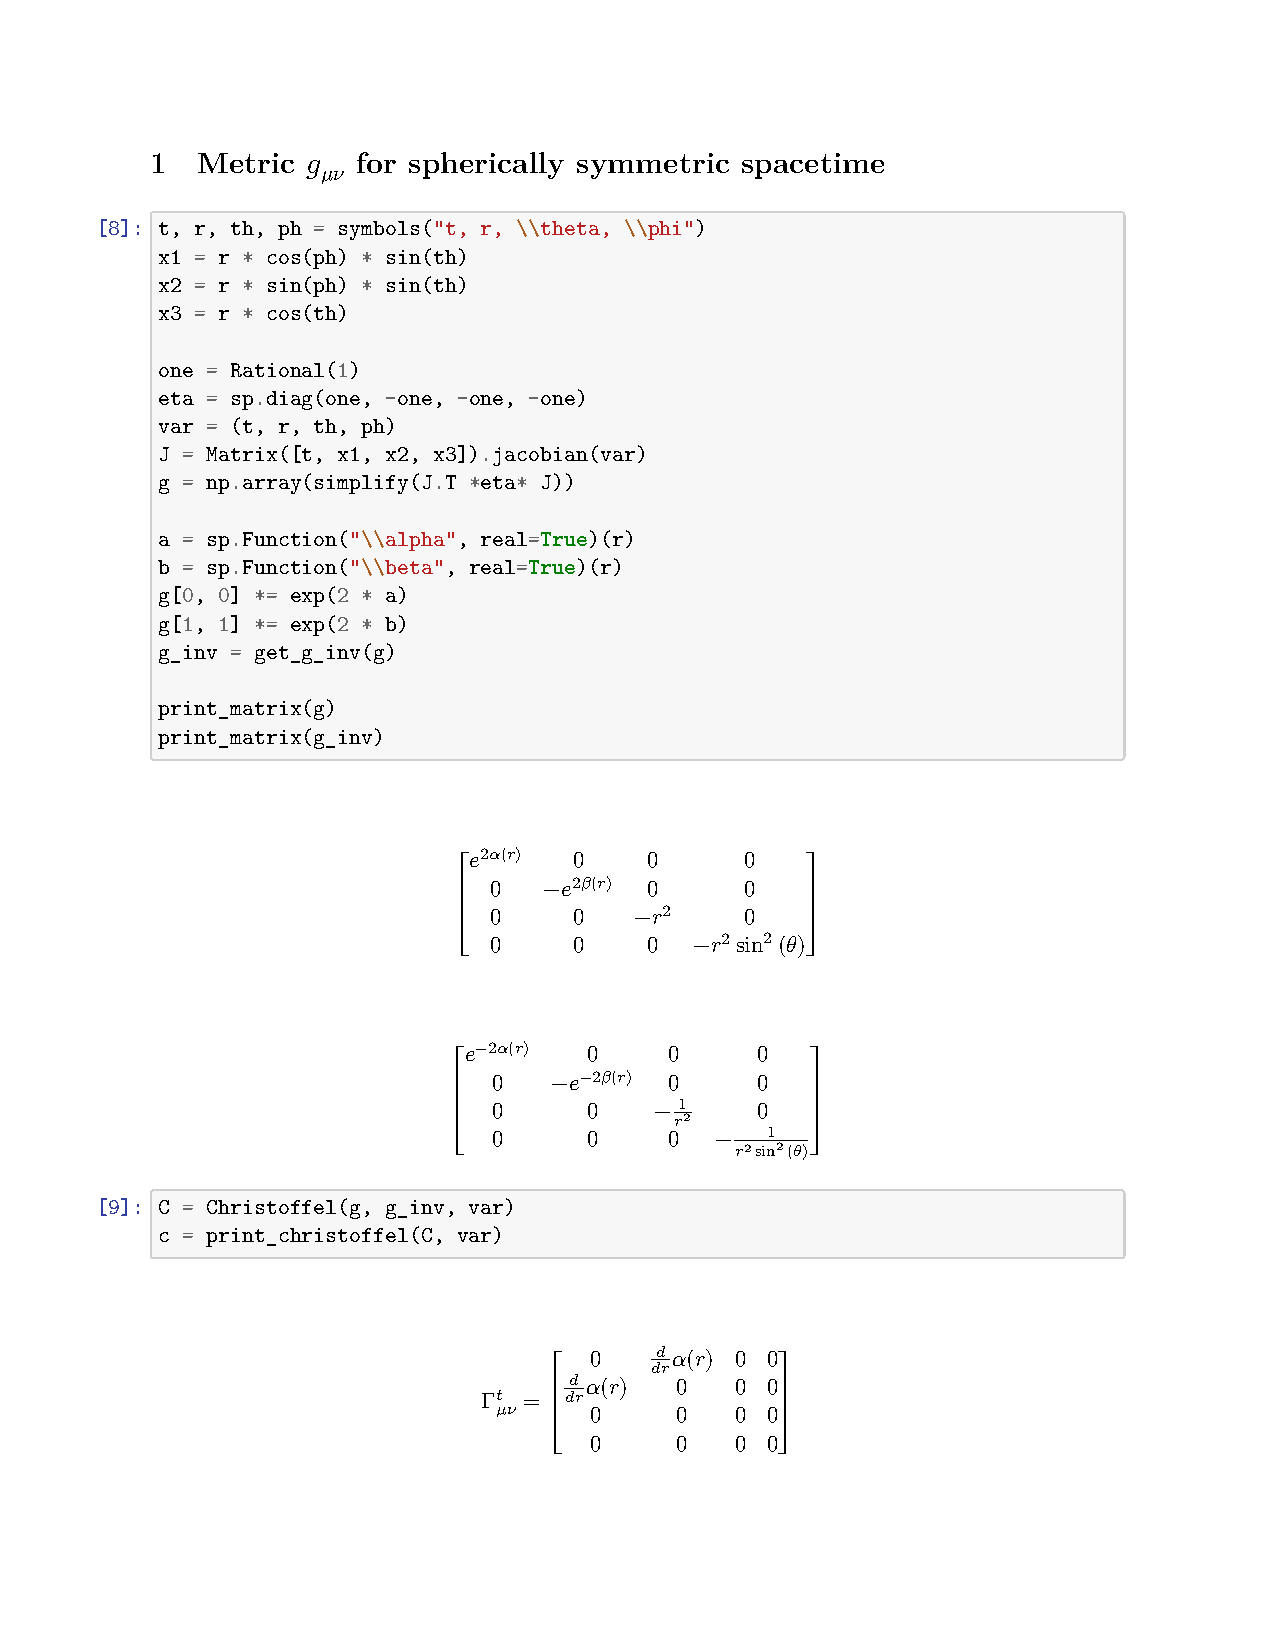
\includepdf[pages=-,pagecommand={},width=1.3\textwidth]{../scripts/TOV/TOV.pdf}




\section{Symbolic calculations in \chpt}
\label{section: symbolic calculations}

Symbolic calculations in \chpt, such as the expansion of the Lagrangian in $\varphi$, were done using the open-source, Python-based case SageMath\footnote{\url{https://www.sagemath.org/}}, and jupyter notebook\footnote{\url{https://jupyter.org/}}.
The calculations consisted of expanding the Lagrangian in a series of $\varphi_a/f$.
The calculations presented in this thesis, in addition to expansions of $\Ell_4$ to second order, can be found in the online repository, at \url{https://github.com/martkjoh/master/tree/main/power_expansion}.



    \printbibliography

\end{document}
